

% Note that the a4paper option is mainly intended so that authors in
% countries using A4 can easily print to A4 and see how their papers will
% look in print - the typesetting of the document will not typically be
% affected with changes in paper size (but the bottom and side margins will).
% Use the testflow package mentioned above to verify correct handling of
% both paper sizes by the user's LaTeX system.
%
% Also note that the "draftcls" or "draftclsnofoot", not "draft", option
% should be used if it is desired that the figures are to be displayed in
% draft mode.
%
\documentclass[journal,final,letterpaper,twoside,twocolumn]{IEEEtran}
%\documentclass[journal,final,letterpaper,twoside,twocolumn]{IEEEtran}
% Add the compsoc option for Computer Society conferences.
%
% If IEEEtran.cls has not been installed into the LaTeX system files,
% manually specify the path to it like:
% \documentclass[conference]{../sty/IEEEtran}

\usepackage[utf8]{inputenc}        % Keybord settings


% Some very useful LaTeX packages include:
% (uncomment the ones you want to load)


% *** MISC UTILITY PACKAGES ***
%
%\usepackage{ifpdf}
% Heiko Oberdiek's ifpdf.sty is very useful if you need conditional
% compilation based on whether the output is pdf or dvi.
% usage:
% \ifpdf
%   % pdf code
% \else
%   % dvi code
% \fi
% The latest version of ifpdf.sty can be obtained from:
% http://www.ctan.org/tex-archive/macros/latex/contrib/oberdiek/
% Also, note that IEEEtran.cls V1.7 and later provides a builtin
% \ifCLASSINFOpdf conditional that works the same way.
% When switching from latex to pdflatex and vice-versa, the compiler may
% have to be run twice to clear warning/error messages.






% *** CITATION PACKAGES ***
%
\usepackage{cite}
\usepackage{textcomp}

% cite.sty was written by Donald Arseneau
% V1.6 and later of IEEEtran pre-defines the format of the cite.sty package
% \cite{} output to follow that of IEEE. Loading the cite package will
% result in citation numbers being automatically sorted and properly
% "compressed/ranged". e.g., [1], [9], [2], [7], [5], [6] without using
% cite.sty will become [1], [2], [5]--[7], [9] using cite.sty. cite.sty's
% \cite will automatically add leading space, if needed. Use cite.sty's
% noadjust option (cite.sty V3.8 and later) if you want to turn this off.
% cite.sty is already installed on most LaTeX systems. Be sure and use
% version 4.0 (2003-05-27) and later if using hyperref.sty. cite.sty does
% not currently provide for hyperlinked citations.
% The latest version can be obtained at:
% http://www.ctan.org/tex-archive/macros/latex/contrib/cite/
% The documentation is contained in the cite.sty file itself.






% *** GRAPHICS RELATED PACKAGES ***
%
\ifCLASSINFOpdf
  \usepackage[pdftex]{graphicx}
  % declare the path(s) where your graphic files are
  % \graphicspath{{../pdf/}{../jpeg/}}
  % and their extensions so you won't have to specify these with
  % every instance of \includegraphics
  % \DeclareGraphicsExtensions{.pdf,.jpeg,.png}
\else
  % or other class option (dvipsone, dvipdf, if not using dvips). graphicx
  % will default to the driver specified in the system graphics.cfg if no
  % driver is specified.
 \usepackage[dvips]{graphicx}
  % declare the path(s) where your graphic files are
  % \graphicspath{{../eps/}}
  % and their extensions so you won't have to specify these with
  % every instance of \includegraphics
  % \DeclareGraphicsExtensions{.eps}
\fi
% graphicx was written by David Carlisle and Sebastian Rahtz. It is
% required if you want graphics, photos, etc. graphicx.sty is already
% installed on most LaTeX systems. The latest version and documentation can
% be obtained at:
% http://www.ctan.org/tex-archive/macros/latex/required/graphics/
% Another good source of documentation is "Using Imported Graphics in
% LaTeX2e" by Keith Reckdahl which can be found as epslatex.ps or
% epslatex.pdf at: http://www.ctan.org/tex-archive/info/
%
% latex, and pdflatex in dvi mode, support graphics in encapsulated
% postscript (.eps) format. pdflatex in pdf mode supports graphics
% in .pdf, .jpeg, .png and .mps (metapost) formats. Users should ensure
% that all non-photo figures use a vector format (.eps, .pdf, .mps) and
% not a bitmapped formats (.jpeg, .png). IEEE frowns on bitmapped formats
% which can result in "jaggedy"/blurry rendering of lines and letters as
% well as large increases in file sizes.
%
% You can find documentation about the pdfTeX application at:
% http://www.tug.org/applications/pdftex





% *** MATH PACKAGES ***
%
\usepackage[cmex10]{amsmath}
% A popular package from the American Mathematical Society that provides
% many useful and powerful commands for dealing with mathematics. If using
% it, be sure to load this package with the cmex10 option to ensure that
% only type 1 fonts will utilized at all point sizes. Without this option,
% it is possible that some math symbols, particularly those within
% footnotes, will be rendered in bitmap form which will result in a
% document that can not be IEEE Xplore compliant!
%
% Also, note that the amsmath package sets \interdisplaylinepenalty to 10000
% thus preventing page breaks from occurring within multiline equations. Use:
%\interdisplaylinepenalty=2500
% after loading amsmath to restore such page breaks as IEEEtran.cls normally
% does. amsmath.sty is already installed on most LaTeX systems. The latest
% version and documentation can be obtained at:
% http://www.ctan.org/tex-archive/macros/latex/required/amslatex/math/





% *** SPECIALIZED LIST PACKAGES ***
%
%\usepackage{algorithmic}
% algorithmic.sty was written by Peter Williams and Rogerio Brito.
% This package provides an algorithmic environment fo describing algorithms.
% You can use the algorithmic environment in-text or within a figure
% environment to provide for a floating algorithm. Do NOT use the algorithm
% floating environment provided by algorithm.sty (by the same authors) or
% algorithm2e.sty (by Christophe Fiorio) as IEEE does not use dedicated
% algorithm float types and packages that provide these will not provide
% correct IEEE style captions. The latest version and documentation of
% algorithmic.sty can be obtained at:
% http://www.ctan.org/tex-archive/macros/latex/contrib/algorithms/
% There is also a support site at:
% http://algorithms.berlios.de/index.html
% Also of interest may be the (relatively newer and more customizable)
% algorithmicx.sty package by Szasz Janos:
% http://www.ctan.org/tex-archive/macros/latex/contrib/algorithmicx/




% *** ALIGNMENT PACKAGES ***
%
%\usepackage{array}
% Frank Mittelbach's and David Carlisle's array.sty patches and improves
% the standard LaTeX2e array and tabular environments to provide better
% appearance and additional user controls. As the default LaTeX2e table
% generation code is lacking to the point of almost being broken with
% respect to the quality of the end results, all users are strongly
% advised to use an enhanced (at the very least that provided by array.sty)
% set of table tools. array.sty is already installed on most systems. The
% latest version and documentation can be obtained at:
% http://www.ctan.org/tex-archive/macros/latex/required/tools/


%\usepackage{mdwmath}
%\usepackage{mdwtab}
% Also highly recommended is Mark Wooding's extremely powerful MDW tools,
% especially mdwmath.sty and mdwtab.sty which are used to format equations
% and tables, respectively. The MDWtools set is already installed on most
% LaTeX systems. The lastest version and documentation is available at:
% http://www.ctan.org/tex-archive/macros/latex/contrib/mdwtools/


% IEEEtran contains the IEEEeqnarray family of commands that can be used to
% generate multiline equations as well as matrices, tables, etc., of high
% quality.


%\usepackage{eqparbox}
% Also of notable interest is Scott Pakin's eqparbox package for creating
% (automatically sized) equal width boxes - aka "natural width parboxes".
% Available at:
% http://www.ctan.org/tex-archive/macros/latex/contrib/eqparbox/





% *** SUBFIGURE PACKAGES ***
%\usepackage[tight,footnotesize]{subfig}
% subfigure.sty was written by Steven Douglas Cochran. This package makes it
% easy to put subfigures in your figures. e.g., "Figure 1a and 1b". For IEEE
% work, it is a good idea to load it with the tight package option to reduce
% the amount of white space around the subfigures. subfigure.sty is already
% installed on most LaTeX systems. The latest version and documentation can
% be obtained at:
% http://www.ctan.org/tex-archive/obsolete/macros/latex/contrib/subfigure/
% subfigure.sty has been superceeded by subfig.sty.



\usepackage[caption=false]{caption}
\usepackage[font=footnotesize]{subfig}
% subfig.sty, also written by Steven Douglas Cochran, is the modern
% replacement for subfigure.sty. However, subfig.sty requires and
% automatically loads Axel Sommerfeldt's caption.sty which will override
% IEEEtran.cls handling of captions and this will result in nonIEEE style
% figure/table captions. To prevent this problem, be sure and preload
% caption.sty with its "caption=false" package option. This is will preserve
% IEEEtran.cls handing of captions. Version 1.3 (2005/06/28) and later
% (recommended due to many improvements over 1.2) of subfig.sty supports
% the caption=false option directly:
%\usepackage[caption=false,font=footnotesize]{subfig}
%
% The latest version and documentation can be obtained at:
% http://www.ctan.org/tex-archive/macros/latex/contrib/subfig/
% The latest version and documentation of caption.sty can be obtained at:
% http://www.ctan.org/tex-archive/macros/latex/contrib/caption/




% *** FLOAT PACKAGES ***
%
%\usepackage{fixltx2e}
% fixltx2e, the successor to the earlier fix2col.sty, was written by
% Frank Mittelbach and David Carlisle. This package corrects a few problems
% in the LaTeX2e kernel, the most notable of which is that in current
% LaTeX2e releases, the ordering of single and double column floats is not
% guaranteed to be preserved. Thus, an unpatched LaTeX2e can allow a
% single column figure to be placed prior to an earlier double column
% figure. The latest version and documentation can be found at:
% http://www.ctan.org/tex-archive/macros/latex/base/



%\usepackage{stfloats}
% stfloats.sty was written by Sigitas Tolusis. This package gives LaTeX2e
% the ability to do double column floats at the bottom of the page as well
% as the top. (e.g., "\begin{figure*}[!b]" is not normally possible in
% LaTeX2e). It also provides a command:
%\fnbelowfloat
% to enable the placement of footnotes below bottom floats (the standard
% LaTeX2e kernel puts them above bottom floats). This is an invasive package
% which rewrites many portions of the LaTeX2e float routines. It may not work
% with other packages that modify the LaTeX2e float routines. The latest
% version and documentation can be obtained at:
% http://www.ctan.org/tex-archive/macros/latex/contrib/sttools/
% Documentation is contained in the stfloats.sty comments as well as in the
% presfull.pdf file. Do not use the stfloats baselinefloat ability as IEEE
% does not allow \baselineskip to stretch. Authors submitting work to the
% IEEE should note that IEEE rarely uses double column equations and
% that authors should try to avoid such use. Do not be tempted to use the
% cuted.sty or midfloat.sty packages (also by Sigitas Tolusis) as IEEE does
% not format its papers in such ways.




% *** PDF, URL AND HYPERLINK PACKAGES ***
%
%\usepackage{url}
% url.sty was written by Donald Arseneau. It provides better support for
% handling and breaking URLs. url.sty is already installed on most LaTeX
% systems. The latest version can be obtained at:
% http://www.ctan.org/tex-archive/macros/latex/contrib/misc/
% Read the url.sty source comments for usage information. Basically,
% \url{my_url_here}.





% *** Do not adjust lengths that control margins, column widths, etc. ***
% *** Do not use packages that alter fonts (such as pslatex).         ***
% There should be no need to do such things with IEEEtran.cls V1.6 and later.
% (Unless specifically asked to do so by the journal or conference you plan
% to submit to, of course. )


% correct bad hyphenation here
\hyphenation{op-tical net-works semi-conduc-tor middle-ware}

\newcommand{\hide}[1]{}
\begin{document}
%
% paper title
% can use linebreaks \\ within to get better formatting as desired
\title{Navigation Strategy and Trajectory Following Controller for an Autonomous Sailing Vessel}



% author names and affiliations
% use a multiple column layout for up to three different
% affiliations



%\author{

%\IEEEauthorblockN{Sebastian Boehl\IEEEauthorrefmark{1}}

%\and

%\IEEEauthorblockN{Lian P. Giger}
%\IEEEauthorblockA{ETH\\Federal Institute of Technology\\
%Zurich, Switzerland\\
%Email: ligiger@student.ethz.ch}

%\and

%\IEEEauthorblockN{Stefan Wismer} \IEEEauthorblockA{ETH Zurich}}

% conference papers do not typically use \thanks and this command
% is locked out in conference mode. If really needed, such as for
% the acknowledgment of grants, issue a \IEEEoverridecommandlockouts
% after \documentclass

% for over three affiliations, or if they all won't fit within the width
% of the page, use this alternative format:
%
\author{\IEEEauthorblockN{Hendrik Erckens ({\small corresponding author}), Gion-Andri Büsser,\\Dr. C\'{e}dric Pradalier, Prof Dr. Roland Y. Siegwart\\ \IEEEauthorblockA{Autonomous Systems Lab, Swiss Federal
Institute of Technology (ETH) Zurich\\Leonhardstrasse 25, 8092 Zurich, Switzerland \\
E-mail: herckens@student.ethz.ch}}}

% use for special paper notices
%\IEEEspecialpapernotice{(Invited Paper)}

% make the title area
\maketitle
\begin{abstract}
%\boldmath
This paper describes the design and implementation of a navigation and control
system for the autonomous sailing
vessel {\sc Avalon}. This boat, designed for participating in the {\sc
Microtransat}, is engineered to autonomously cross the Atlantic Ocean. We
present here a specially robust mechanical design and the navigation software
that will plan an optimal navigation course and efficiently control the boat on
this course. The path planner uses an A* algorithm to generate the fastest path
to a given destination. It is able to avoid both static and dynamic obstacles.
By using a given polar diagram and measured wind data, it takes into account
manoeuvrability constraints of a sailboat. The control system takes care of
rudder and sail in order to follow a given heading while optimising speed.
Additionally, the system is capable of automatically conducting manoeuvres such
as tack and jibe. 
At the time of this writing, {\sc Avalon} and its software systems have been
successfully tested more than two weeks in short deployments lasting several
hours with winds ranging from 0 up to 30 knots. 
\end{abstract}
% IEEEtran.cls defaults to using nonbold math in the Abstract.
% This preserves the distinction between vectors and scalars. However,
% if the conference you are submitting to favors bold math in the abstract,
% then you can use LaTeX's standard command \boldmath at the very start
% of the abstract to achieve this. Many IEEE journals/conferences frown on
% math in the abstract anyway.
%
% no keywords
%
% For peer review papers, you can put extra information on the cover
% page as needed:
% \ifCLASSOPTIONpeerreview
% \begin{center} \bfseries EDICS Category: 3-BBND \end{center}
% \fi
%
% For peerreview papers, this IEEEtran command inserts a page break and
% creates the second title. It will be ignored for other modes.
% \IEEEpeerreviewmaketitle
%
\section{Introduction}
%\subsection{General Objectives for building an autonomous sailboat}
This paper introduces the autonomous sailboat \textsc{Avalon} as seen in figure
\ref{fig:avalon}. The general objective for building an autonomous sailing
vessel is to further research and development in the area of unmanned,
autonomous robotic vehicles that are exposed to heavy environmental conditions
such as the Atlantic Ocean. It has been established that there is a demand for
autonomous sailboats to be used for ocean sampling and surveillance
\cite{cruz:ase} but also for the implementation of this type of software in
manned sailing vessels. Either by passively proposing optimal sailing routes or
by actively supporting the sailor in dangerous situations by piloting the sail
or rudders, an integrated autonomous sailing system could back up and
facilitate a lot of situations. For example, if a single hand sailor falls over
board, the system could detect this incident and automatically execute a Man
Over Board manoeuvre.

\subsection{Our Goals and Objectives for this Work}
Our boat \textsc{Avalon} was designed to compete in the \textsc{Microtransat}
Challenge and thus has to withstand the harsh conditions on the Atlantic Ocean.

The goal of this paper is to present a software that is
capable of calculating the optimal path to reach a given destination as quickly
as possible, and the design of a controller able to safely and efficiently
guide the sailboat along the calculated path, taking into account the current
environmental conditions, such as wind speed.
\hide{Furthermore, it should be able to respond to a possible shortness of
energy by adjusting the control parameters or changing the mode of sailing.}


\subsection{Review of Existing Autonomous Sailing Boats}
An autonomous sailboat has to be capable of sailing without human intervention.
That means, that all tasks that are normally carried out by the sailor on a
conventional sailboat have to be done autonomously. That involves navigation
as well as working the rudder and sail in order to steer the defined course.
Other autonomous sailboats have been developed mostly by \textsc{Microtransat}
participants \cite{briere2008iar}, \cite{stelzer2008}, \cite{alves:fas},
\cite{sauze2008dcs}, but also commercially usable products \cite{harborwing}
have been built. In contrast to most of the existing work, we use a path
planner to avoid obstacles. Additionally, our controller switches between many
different modes of sailing, in order to make better use of wind shifts.

\section{A Boat Designed for Survival}
To provide an insight into the platform that was used to implement the proposed
software, this section summarises some details about the main components of
{\sc Avalon}. The mechanical system was more comprehensively described in
\cite{giger2009}. Table \ref{tab:avalon_data} shows the major technical details
of {\sc Avalon}.
\begin{figure}[b!]
\centering
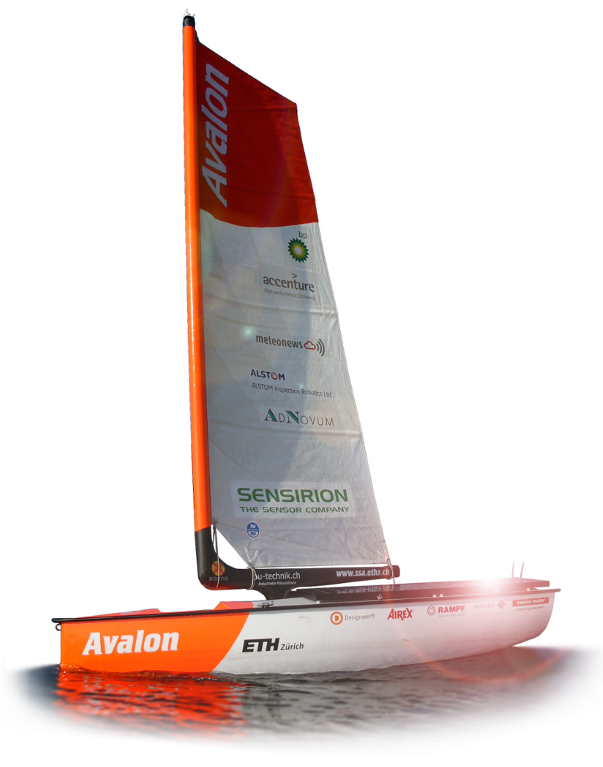
\includegraphics[height=0.8\columnwidth]{pics/avalon.png}
\caption{Avalon ready to sail on the lake of Z\"urich}
\label{fig:avalon}
\end{figure}

\subsection{Rig}
The rigging system is one of the most important parts of the whole
assembly. A defect in its structure will inevitably cause the whole project to
fail. The following aspects were considered for the design:
\begin{itemize}
\item High loads and forces on the mechanical structures due to
strong winds and heavy weather conditions.
\item Highest demands on reliability. There is no chance to
repair anything throughout the journey.
\item Preferably efficient force transmission from the actuator to the sail in order to save as much energy as
possible
\end{itemize}

During the design phase it turned out that a balanced rig prevails over a
conventional rig.
\hide{
The balanced rig is much more efficient regarding energy
consumption than any other conventional rig. The force needed to position the
sail is reduced by over 50\% due to the balanced distribution of
the sail load. Furthermore, }\textsc{Avalon}'s rig does not use any ropes
that could generate knots and jams. It is pivoted on a central
bearing without shrouds and stays. The result is a simple and reliable construction.
%
\subsection{Hull}
\hide{The hull design is based on form parameters, e.g. length, draft and
beam. Parameters were used as input data for B-spline curves and
surfaces. Instead of modifying those curves and surfaces, we used
constrained optimisation algorithms to generate the geometry. The algorithm
minimises a target function, which is defined so that a certain combination of
parameters results in a desired hull shape.}

The hull was designed using the CAE software \textsc{FRIENDSHIP-Framework} and
was laminated inside a female mold using glass fibre
sandwich. Epoxide resin was sucked into dry glass fibre material by
vacuum in a so called \textit{Infusion Process}. Compared to
conventional laminating, this method is much cleaner and more
convenient.

%---------------------------------------------------------
%basicdata: AVALON
%---------------------------------------------------------
\begin{table}[htb]

    \begin{center}
     \caption{Technical Data of \textsc{Avalon}}
	\label{tab:avalon_data}
%        \begin{tabular}[h!]{p{0.15\textwidth}| p{0.2\textwidth}| p{0.05\textwidth}}
        \begin{tabular}[htb]{l|l|l}
            \hline
            \emph{Variable}    &   \emph{Description} &   \emph{Value}\\ \hline\hline
            $L_{OA}$    &   Length over all	& $3.95\,m$\\
            $B_{max}$   &   Maximal beam	& $0.7\,m$\\
            $T$         &   Draft without keel  & $0.25\,m$\\
            $D_{max}$	&   Draft over all	& $2\,m$\\
            $H_{rigg}$	&   Height of the rigg  & $5.7\,m$\\
            $A_{sail}$	&   Total sail area     & $8.4\,m^2$\\
            $\nabla$    &   Submerged volume    & $0.44\,m^3$\\
            \hline
        \end{tabular}
    \end{center}
\end{table}


\begin{figure}[htb]
\centering
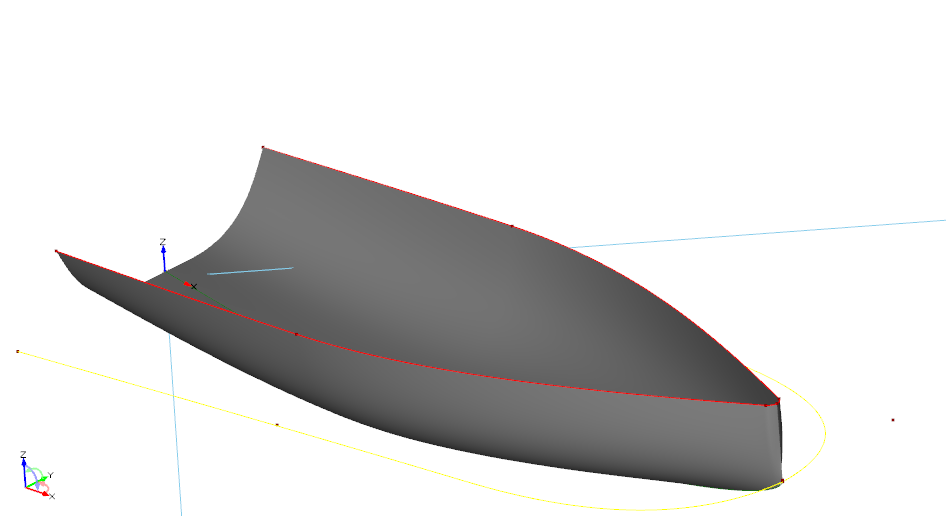
\includegraphics[width=0.37\textwidth]{pics/hull.png}
\caption{Hull} \label{fig:hull}
\end{figure}

%
\subsection{Keel and Rudder}
\subsubsection{Keel}
In order to achieve a sufficient righting moment and stability
during heavy weather situations, {\sc Avalon}'s keel with a draft of
two meters consists of a slim fin with a 160\,kg ballast bulb.

The fin and parts of the bulb were made of high-modulus carbon fibre
in precisely milled polyurethane female molds. After hardening and
tempering, the bulb was filled with lead and the two halves were
glued together.

\begin{figure}[htb]
\centering
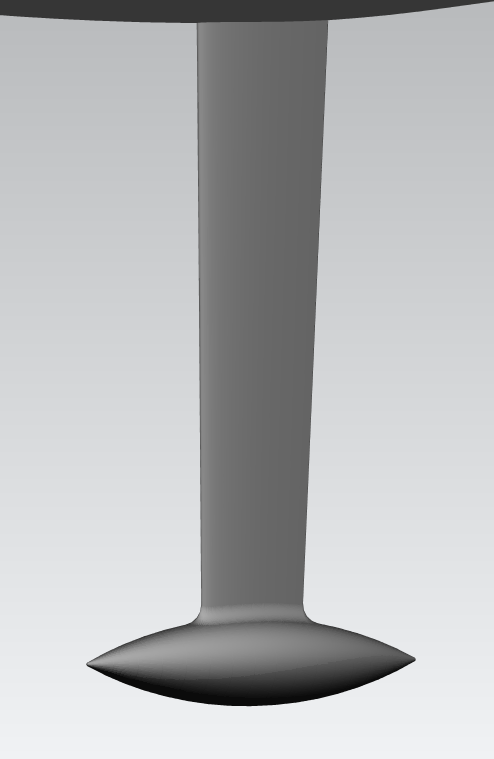
\includegraphics[width=2.7cm]{pics/keel.png}\hfill
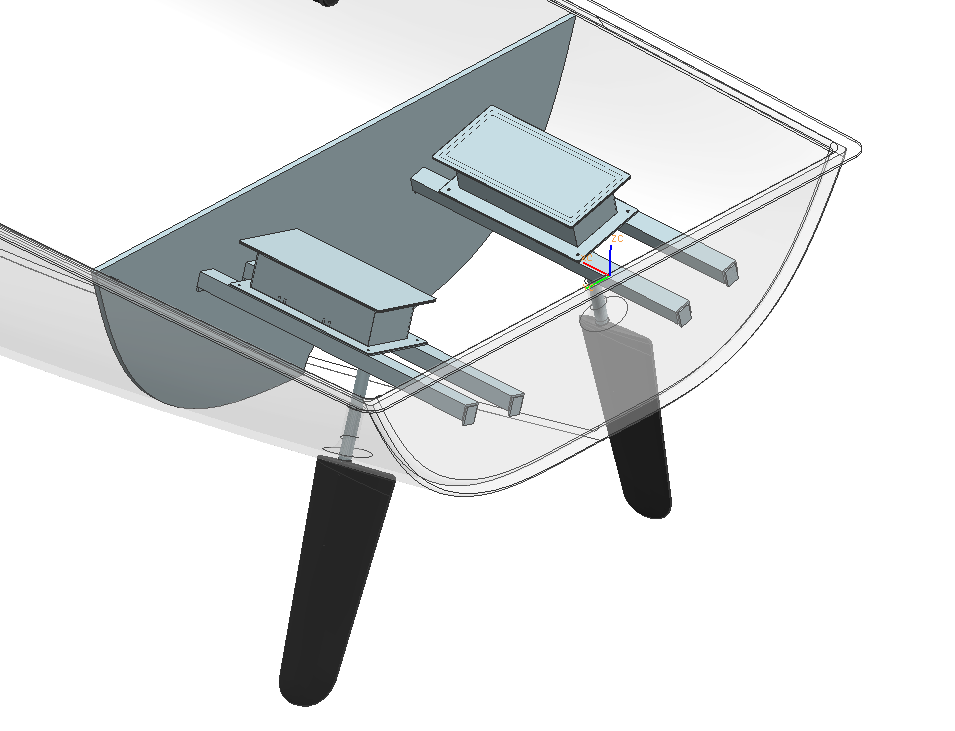
\includegraphics[width=4.5cm]{pics/rudder.png}
% \caption{Twin rudder system} \label{fig:cadrudder}
\caption{Keel with fin and ballast bulb (left), Twin rudder system (right)} \label{fig:cadkeel}
\end{figure}

\subsubsection{Rudder}
A twin-rudder system was selected for {\sc Avalon} to make sure to
have sufficient steering effect in every sailing situation. Angular
mounted twin-rudders provide better control at high
heeling angles compared to single rudders.

Assembled inside the hull, the rudder actuators are well sealed and
protected against water and humidity.

% \begin{figure}[htb]
% \centering
% 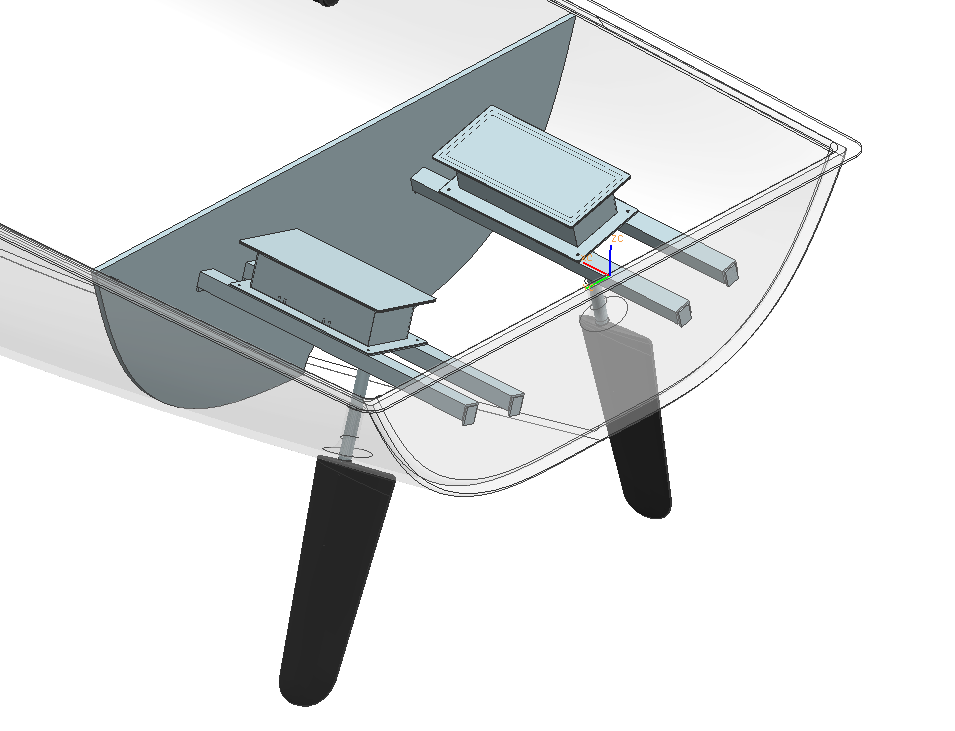
\includegraphics[width=4cm]{pics/rudder.png}
% \caption{Twin rudder system} \label{fig:cadrudder}
% \end{figure}
%
\subsection{Power Supply}
The main power supply is realised through two square meters of solar panels providing
a total of 360\,Wp. The collected energy is stored in four lithium-manganese
batteries. Each battery consists of 70 single cells and has a capacity of
600\,Wh at a nominal voltage of 25.2\,volts. Lithium-manganese batteries were
chosen mainly because of their weight but also because they are fairly safe to
use.

For back-up power, the boat has a direct-methanol fuel cell on
board. This fuel cell is automatically activated when the voltage
drops under a certain value, the \emph{switch on} voltage. It then
charges the batteries until the \emph{switch off} voltage is
reached. In theory, the solar cells provide enough power for the
boat's systems. The fuel cell only serves in case of enduring bad
weather  or other unforeseeable circumstances.



\section{Navigation Stategy}
This chapter will give a general overview of the software developed for
\textsc{Avalon} and discuss the interaction between control system and path
planner. Sections \ref{sec:sailor} and \ref{sec:navigator} will then go further
into details of the actual controller and path planner respectively.

The core hardware part and the brain of the system on the sailing vessel is the
main computer MPC21 from {\sc DigitalLogic}, a 500\,MHz device with 1024\,MB
RAM and a compact flash hard-drive. The device has an average power consumption
of about 8\,watts, the protection of a metal housing and a total weight of less
than 1\,kg.
% \begin{figure}[htb]
% \centering
% 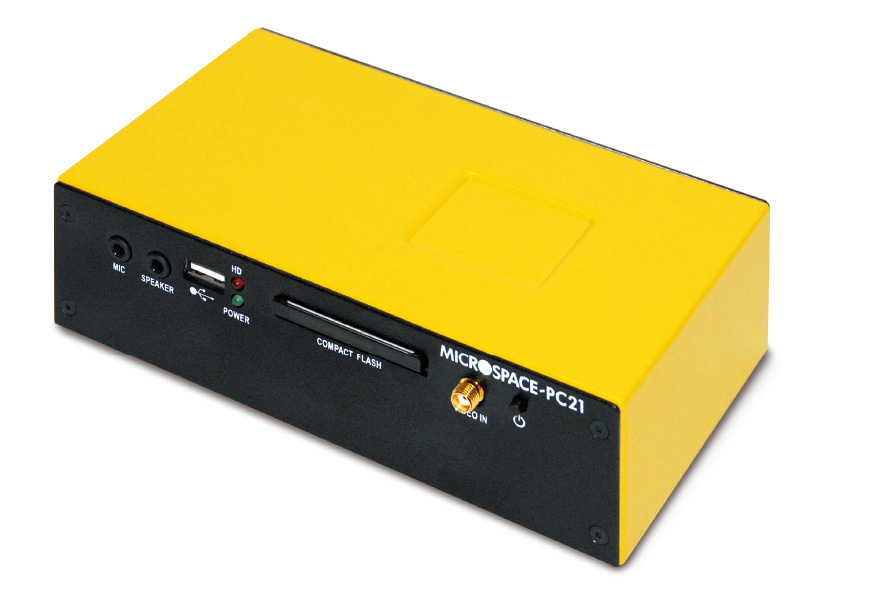
\includegraphics[height=4.0cm]{pics/RE_MPC21.png}\label{fig:mainpc}
% \caption{Main PC and brain of {\sc Avalon}\cite{digitallogic}}
% \end{figure}
%
The base of the entire software structure is the middleware DDX\cite{ddxpaper}
that runs on a Linux Operating System. This software manages a shared memory
called the Store and thus provides a means of communication between individual
programs that all run in parallel (see figure \ref{fig:ddx}). 

Sensor drivers will collect data from the specific sensors (see section
\ref{sec:sensors}) and store it in the DDX Store, from where it can be accessed
by the control and path planning programs.
% 
% A distinct advantage of DDX is the modular software structure. If ever a
% program crashes, it can be restarted without interrupting the other processes.
The different subprograms used on \textsc{Avalon} are depicted in figure
\ref{fig:ddx}.

\begin{figure}[htb]
\centering
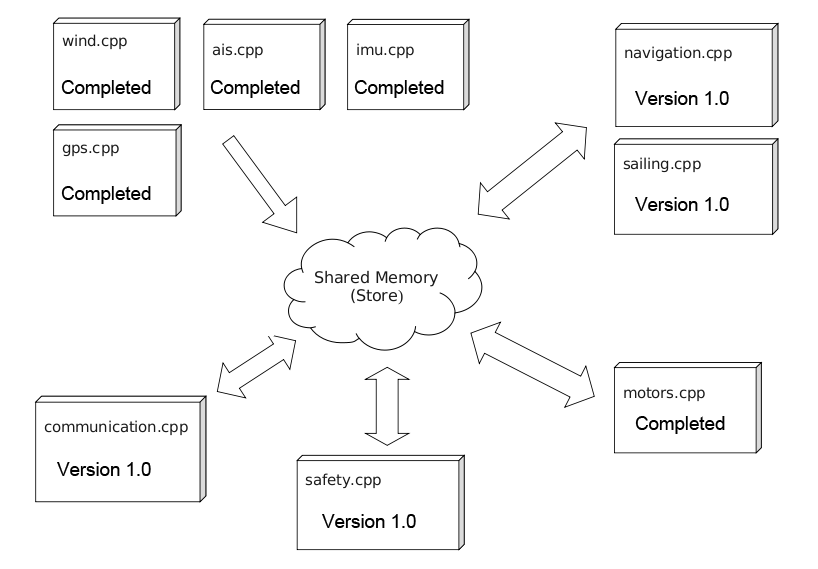
\includegraphics[height=5.5cm]{pics/RE_ddxplain.png}
\caption{Software organisation} \label{fig:ddx}
\end{figure}

%
%
\subsection{Sensors} \label{sec:sensors}
All desired information such as position, heading or speed are measured by
several sensors located all over the boat. To get a fully controllable system,
data is collected from the following sensors:
%
%\begin{description}[\IEEEsetlabelwidth{Wind}\IEEEusemathlabelsep]
%\item[\textbf{GPS}] 
\subsubsection{GPS \& IMU} 
%Provides position, heading and speed. The sensor's antenna is mounted on top of the mast. The electronic unit is located in the hull.
%\item[\textbf{IMU}]
The localization of the boat is performed by an \textit{Inertial Measurement
Unit} (by \textsc{X-Sens}) that is combined with a GPS receiver. Using the
accelerations in all 6 degrees of freedom and a high update rate of 120 Hz,
occasional deviations of the GPS-data will automatically be smoothed out. The
system therefore produces highly accurate positioning.
%
%\item[\textbf{Wind}]
\subsubsection{Wind} Mounted on top of the mast, the wind-sensor provides wind
speed and direction. {\sc Avalon} has an ultrasonic wind-sensor that promises
less mechanical failure than a conventional sensor with a turning wheel. The
sensor by Danish company \textsc{Deif} is IP-66 approved and connected to the
main computer via a RS-485 interface.
%\item[\textbf{AIS}]
\subsubsection{AIS} This Sensor receives data such as position and velocity
from other boats via VHF. The AIS system is an additional means of perception
that ensures that collisions with large commercial ships are avoided.
%\end{description}
%
\subsection{Navigation Management} \label{sec:skipper}
The overall navigation management is being performed by a program further
referred to as trajectory tracker. It's two main tasks are to trigger the local
planner of the path planning algorithm (see section \ref{sec:navigator}) and to
extract from a planned path a sailable boat heading that can be followed by the
controller (see section \ref{sec:sailor}).

The program keeps track of the boat's location as well as it's environment. In
case of predefined emergency cases, it is able to set new destination coordinates.

Having a state machine architecture, the trajectory tracker can switch between
the following states:
%
\subsubsection{Standard Navigation}
If not approaching a target\hide{ or buoy}, this state generates headings for the
control system, going from way-point to way-point. If the wind changes more than $20$°
or if the ship distances itself from the current trajectory for more than a
predefined distance, a new calculation will be initiated. 
\subsubsection{Goal Approach}
If approaching a target position, the trajectory tracker will always send a
heading that is directing exactly towards that point.
\hide{\subsubsection{Buoy Approach}
This is a state designed especially for short course racing. Due to regulations
that always require a port-side surrounding of the regatta buoys, this state
will - when approaching a buoy - always write a heading that will lead the boat
around the buoy.}
\subsubsection{New Calculation}
In this state, the trajectory tracker manages and supervises the new
calculation. After having checked that the new way-points have been stored, it
switches back to \textit{Standard Navigation}
%
%

\section{Control System}\label{sec:sailor}
\subsection{Objectives}
This section describes the design of a controller that is capable of robustly
steering a sailboat along a predefined course while always setting the sail to
the optimal angle to the wind in order to generate as much driving force as
possible. For that, it also has to be able to conduct manoeuvres such as tack
and jibe. At the same time, the controller should take into account the
changing environmental conditions, such as wind speed and direction and react
accordingly. Furthermore, since the path planner (section \ref{sec:navigator})
calculates a global trajectory and relies on the control system to follow this
course, the control system has to compensate for drift.
%
\subsection{Existing Works}
There are various systems available that assist a sailor in steering a
sailboat. Most of these are commercially available autopilots, that operate
either with a built in magnetic compass or with a wind vane
\cite{hochseeportverband1958s}. These systems are finished products, that have
been used for many years and are very robust and reliable. We did not use
commercial products, mainly because of interfacing issues. Autopilots are
designed for a human sailor on board who does the navigation and has to tune
the sails. Although some of the systems are even able to perform tacks and
jibes, the manoeuvre has to be confirmed by the human sailor pressing a button
on the autopilot's control panel. Since the software integrated in commercial
autopilots is typically closed source, this problem cannot be solved by simply
reprogramming the device. Furthermore, most autopilots only control the rudder,
so we would still have to figure out a way to tune the sail.

Apart from the commercial products, there are also several scientific works
regarding control systems for autonomous sailboats, most of them also by
participants in the \textsc{Microtransat}. Developments reach from a fuzzy
logic controller for both rudder and sail \cite{stelzerFuzzy}, over an LQG
controller based on a non-linear 3 degrees of freedom (DOF) model
\cite{elkaim:ska}, up to a complex self learning AI system that has been
successfully tested on an Open60 racing yacht. Our work is mainly influenced by
Briere \cite{briere2008iar}, who describes a simple controller based on a state
machine.
%
\subsection{System Modelling} In order to design a robust controller and
identify parameters in a controlled environment, a simulator is very helpful.
Although there are several sailing simulators available, most of them are made
for gaming. Rather than having an interface that allows them to be steered by a
self-developed control system, they are meant to be operated by hand. For this
reason we implemented a simulator in Matlab/Simulink.

To gain a general system that could later be extended with boat/wave
interaction, the boat was modelled as a rigid body with full 6 DOF. The system
has 12 state variables: 3 for position, 3 for attitude, 3 for velocity and 3 for
turning rates.  Inputs to the plant are rudder angle
$\gamma_{\text{rudder}}$, sail angle $\gamma_{\text{sail}}$, true wind speed
$v_{\text{wind}\_\text{true}}$ and direction $\Psi_{\text{wind}}$, while
outputs are the boat's position and attitude and their corresponding
derivatives.

Forces were introduced at various points of the boat to model the interactions
between water and hull as well as wind and sail.
% \subsubsection{Gravity}
% The only static force acting on our sailing boat is gravity.
\subsubsection{Sail Force}
In order to calculate the force generated by the sail, the apparent wind angle is needed which is computed in a vector operation from the true wind angle and the boat's velocity. The 2 components of the sail force $F_{sail}$ are then modelled using the standard approximation for air foils in a moving fluid
\begin{equation} \label{eqn:air_foil_lift_drag}
\begin{array}{l}
  F_{\text{sail}\_\text{lift}} = \dfrac{1}{2}\cdot \rho_{\text{air}} \cdot v_{\text{wind}\_\text{app}}^2 \cdot A_{\text{sail}} \cdot c_l(\alpha_{\text{sail}})\\
\\
  F_{\text{sail}\_\text{drag}} = \dfrac{1}{2}\cdot \rho_{\text{air}} \cdot v_{\text{wind}\_\text{app}}^2 \cdot A_{\text{sail}} \cdot c_d(\alpha_{\text{sail}})
\end{array}
\end{equation}
where $\rho_{\text{air}}$ is the density of air, $A_{\text{sail}}$ is the
apparent area of the sail and $c_l$ is the lift coefficient which depends on
the sail's shape and the angle of attack $\alpha_{\text{sail}}$.
\subsubsection{Rudder Force}
The rudder force is also modelled using equation \ref{eqn:air_foil_lift_drag},
just with different parameters. Since the rudders are at the stern of the
boat, the force induces a moment around the vertical axis and thus affects the
boat's heading.
\subsubsection{Resistances}
There are several damping forces that depend on the velocity and rate of turn
of the boat. Those are mainly the resistance of hull and keel in all 3 axes of
translational freedom and the damping of rotations. These are modelled using
the equation
\begin{equation}
  F = d \cdot v^2
\end{equation}
where $v$ is the velocity or rate of turn and $d$ is a parameter that has to be
identified in experiments.

After the first tests with the real boat, we found the real boat behaviour to
be quite different from the simulation. To improve this, more tests and
parameter identification needs to be done. Due to time constraints this has not
been done at the time of this writing.

\subsection{Controller Principle}
In our control system layout, rudder and sail are controlled in two separate
Single Input Single Output (SISO) systems that are assumed to be independent of
each other. During testing, this assumption has proved to be very reasonable.

\subsubsection{Sail Control}
For the sail, the controlled value is the angle of attack. This directly
depends on the sail's angle. Since \textsc{Avalon}'s sail and rudder motors
already come with a built in positioning controller, this subsystem is
sufficiently controlled by just writing a reference value to the motor
controller.

This reference value is derived from a predefined optimal Angle Of Attack (AOA)
that was found in experiments. However, for safety reasons, the wanted AOA also
changes dynamically depending on the wind speed. Basically, as the wind speed
increases, the wanted AOA approaches zero, which reduces the sail force
generated by the wind. With this behaviour, the boat remains steerable even in
strong winds.

\subsubsection{Rudder Control}
The second subsystem controls the boat's heading using the rudder as input.
Since the heading changes dynamically and is not directly dependent on the
rudder angle, this system takes a little more consideration. For this purpose,
a heading error minimising PID controller was designed in an iterative process using the Matlab
simulation. It was then tested and optimised in the real boat (see section
\ref{sec:sailor_testing}).

In order to compensate for leeway drift, the boat has to sail somewhat closer
to the wind than the desired heading $DH_{\text{nav}}$ calculated by the path
planner.
Since drift changes considerably with the wind and wave conditions, it is
important to know the current drift in order to compensate for it. \textsc{Avalon}
is equipped with an Inertial Measurement Unit (IMU) with a built in GPS
receiver. With this sensor, the drift speed $v_{\text{drift}}$ can be accurately
measured at any time. From the drift, a new desired heading DH$_{\text{sailor}}$ is
calculated using the equation
\begin{equation}
  \text{DH}_{\text{sailor}} = \text{DH}_{\text{nav}} + \arctan\left( \frac{v_{\text{drift}}}{v_{\text{boat}}} \right)
\end{equation}

\subsubsection{State Machine}
A sailboat can not sail at all angles to the wind. Figure \ref{fig:courses_to_wind} shows the ranges that we cannot sail in gray. In order to sail as fast as possible, it has to be differentiated between different types of sailing. To this end, the controller is designed as a state machine that switches states depending on the angle to the wind. The 5 states are depicted in figure \ref{fig:courses_to_wind}.
\begin{figure}[htb]
\centering
% trim = left bottom right top
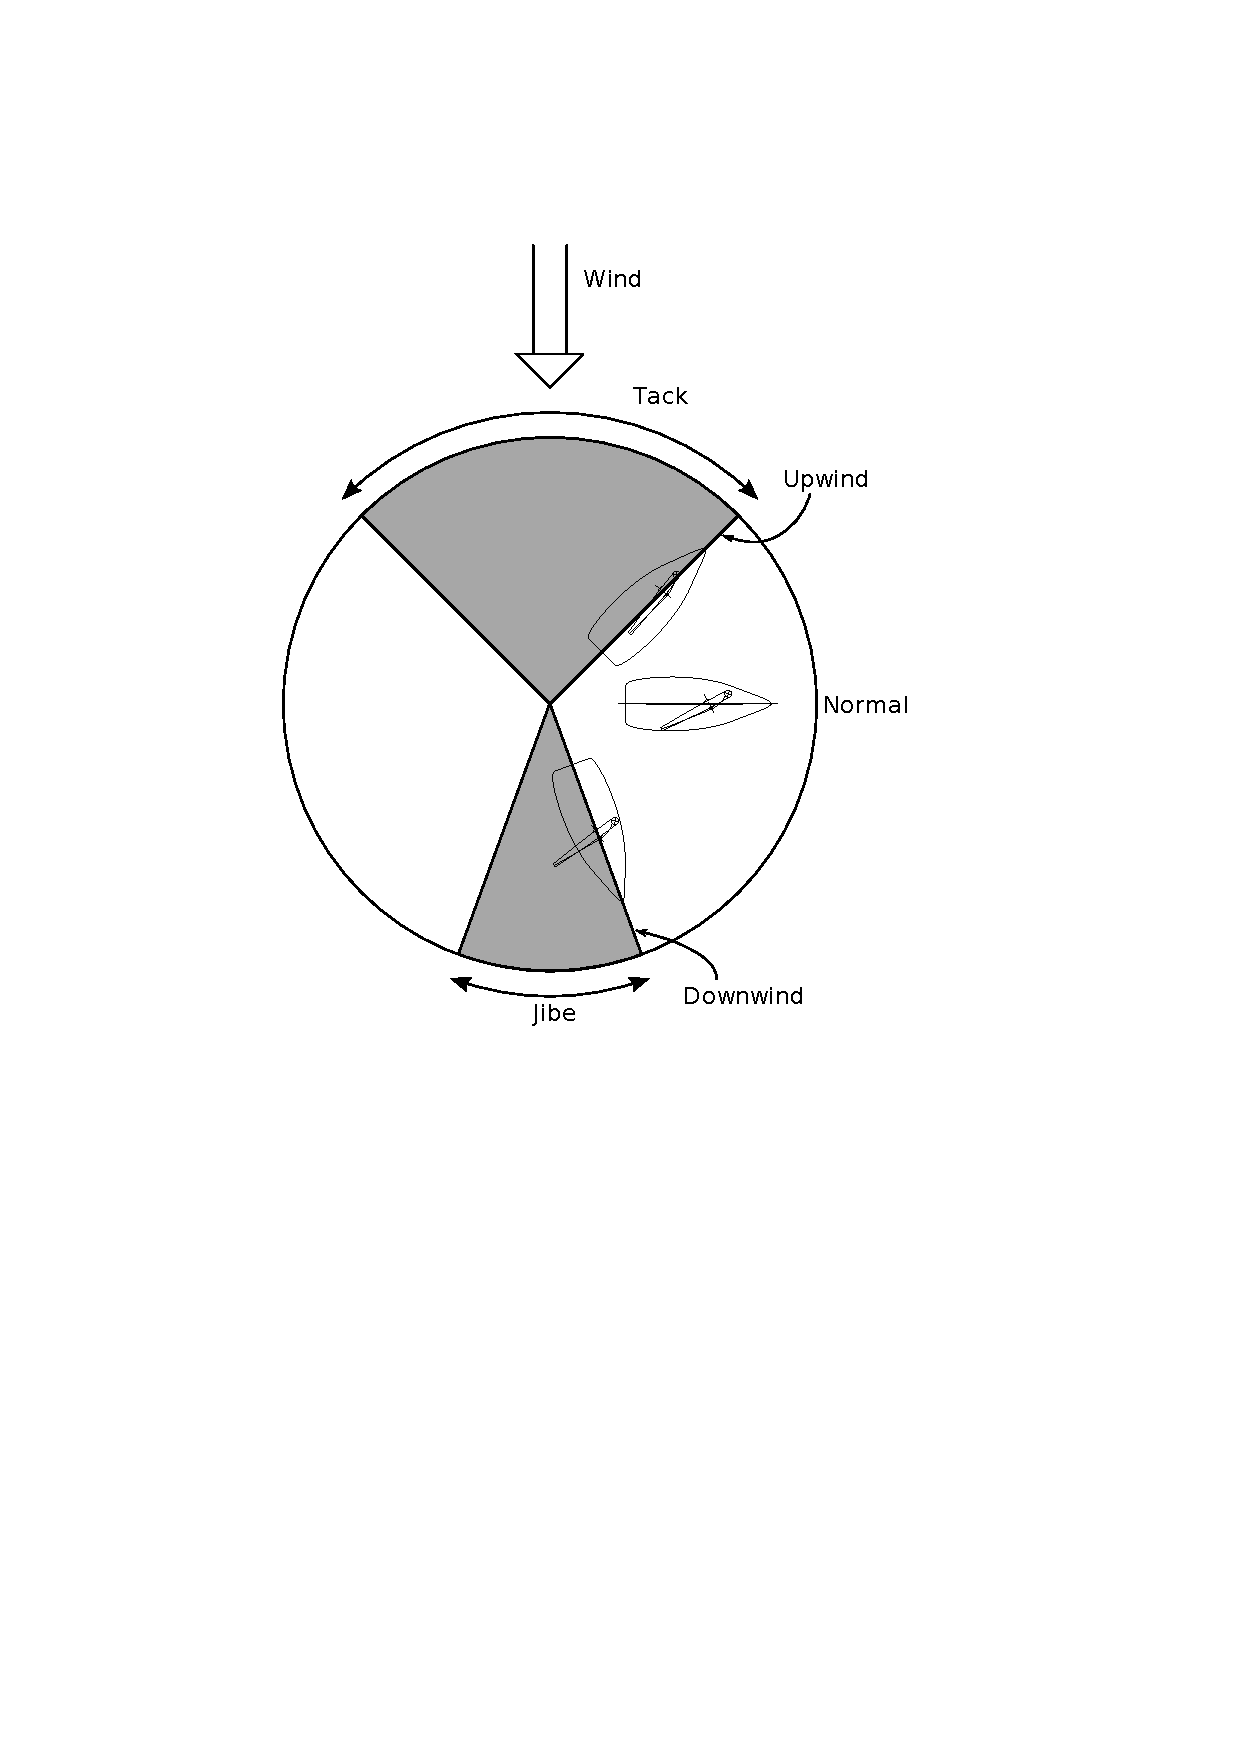
\includegraphics[trim = 45mm 120mm 55mm 45mm, clip, width=0.70\columnwidth]{pics/courses_to_wind.pdf}
\caption{Possible courses of a sailing yacht with respect to the wind and corresponding control system states. The range with wind directly from behind could be sailed in theory, but is not very efficient and rather unstable.}\label{fig:courses_to_wind}
\end{figure}
\subsubsection{Normal Sailing}
If the desired heading given by the path planner (section \ref{sec:navigator}) is
in the sailable (white) range, the system is in state \texttt{Normal Sailing}.
In this state the rudder controller follows the given desired heading, while
the sail controller permanently adjusts the sail to achieve the optimal angle
of attack on the sail. If the desired heading changes within the sailable
range, the rudder controller simply follows the new course while the sail
controller maintains a constant angle of attack.
\subsubsection{Upwind Sailing}
If the desired heading for whatever reason is set in the not sailable (gray)
range, it cannot be directly followed. The objective in this case is to make as
much velocity towards the wind as possible. In \texttt{Upwind Sailing} mode the
sail is set to the tightest position that is reasonably possible. While the
sail angle is kept at this constant position, the rudder controller now keeps a
constant heading angle to the true wind and thus takes advantage of all wind shifts.
Note that the behaviour is similar for downwind sailing.
%
\subsection{Test Results and Analysis} \label{sec:sailor_testing}
Several tests were undertaken to verify and optimise the control system. Before
any testing on the water was done, the state machine's transition conditions
had to be verified. This was done by putting the boat on a trailer on a
sufficiently windy day and turning it around its vertical axis while constantly
checking the current state. We encountered many problems that were caused by
the sign change between $-180^o$ and $+180^o$. Some time could have been saved,
if the whole control program, including the state machine, had been tested more
thoroughly in the simulation environment.

The controller was then tested for its ability to keep a desired heading and to
react to changes in desired heading. After some tuning of the PID parameters we
found that the parameters in table \ref{tab:pid_params} yield fast reactions
without too much overshoot.
%
\begin{table}[htb]
\caption{PID Parameters} \label{tab:pid_params}
\centering
\begin{tabular}{c|l}\hline
P & 0.3  \\ \hline
I & 0.005 \\ \hline
D & 30 \\ \hline
\end{tabular}
\end{table}
%
A step response in winds of about 20 knots is illustrated in figure
\ref{fig:step_response_wind20kn}. Note that 20 knots is already a strong wind
and that in lower wind speeds we experienced much less oscillation around the
reference value. Even this $\pm 10^o$ oscillation that is mostly caused by
waves can barely be seen on the boat. We then also applied disturbances to the
boat by deviating it from its course by hand. The reaction was the same as with
changes in desired heading.
%
\begin{figure}[thb]
\centering
% trim = left bottom right top
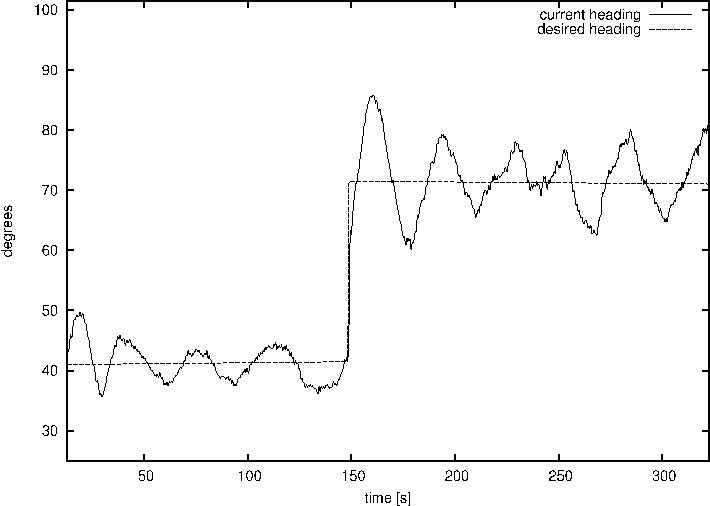
\includegraphics[trim = 0mm 0mm 0mm 0mm, clip, width=7cm]{pics/reference_step_usee4_2.pdf}
\caption{Step response in state \texttt{Normal Sailing}. Conditions were 20\,kn wind from 140°}\label{fig:step_response_wind20kn}
\end{figure}

Figure \ref{fig:3tacks_upwind_sailing} shows current heading, desired heading
and wind direction during three tacks. Between the tacks, the controller state
machine is in state \texttt{Upwind Sailing}. It can be very well seen, that the
boat keeps a constant angle to the wind and takes advantage of wind shifts as
expected.
\begin{figure}[thb]
\centering
% trim = left bottom right top
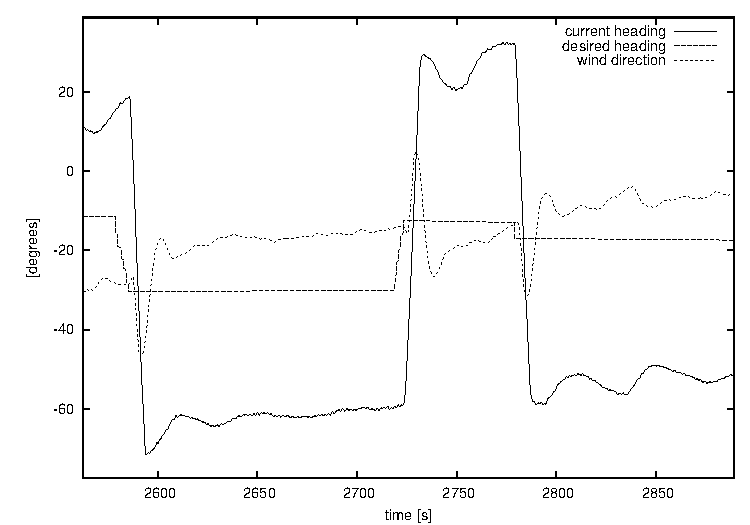
\includegraphics[trim = 0mm 0mm 0mm 0mm, clip, width=7cm]{pics/tacks_to_upwind_usee5_wind8kn_hdg.pdf}
\caption{3 tacks, with \texttt{Upwind Sailing} in between.}\label{fig:3tacks_upwind_sailing}
\end{figure}
A lot of time was invested into correct timing during tack and jibe. In the
beginning we had several problems that resulted in inappropriate sail tuning
during or right after manoeuvres. This sometimes even resulted in the boat
sailing backwards.

Figure \ref{fig:wyp_autonom_drift_comp} shows how the boat follows a trajectory
that was calculated by the path planner. The path planner's calculation was started
at the bottom left where the dashed line begins. After the calculation was
completed, the boat jibes and sets the new course. After a few seconds the
drift compensation starts to work and the boat's real course approaches the
desired trajectory.
%
\begin{figure}[thb]
\centering
% trim = left bottom right top
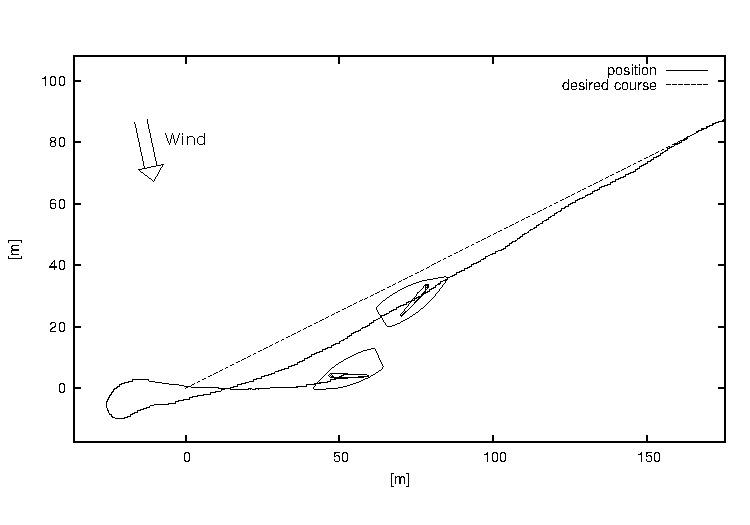
\includegraphics[trim = 0mm 0mm 0mm 0mm, clip, width=7cm]{pics/driftcompensation.pdf}
\caption{GPS plot of the controller following a desired trajectory calculated
by the path planner. It was recorded during a test on the Urnersee in about 15
knots wind.}\label{fig:wyp_autonom_drift_comp}
\end{figure}


\section{Path Planner} \label{sec:navigator}
\subsection{Principle of motion planning for a sailing boat} \label{sec:intro_principle}
Due to the nature of every sailing vessel, \textsc{Avalon}'s manoeuvrability is
limited in relation to wind direction. Additionally, due to the non-holonomic
properties of a sailing vessel, it is not possible to change the heading on the
spot immediately.  The trajectory tracker (see section \ref{sec:skipper}) has
to keep that in mind and operate in a way that allows a certain space to make
heading changes. For the implementation of a navigation algorithm, these
constraints imply that using accurate wind information for every calculation is
essential.
 
\subsection{Literature Research}
%
Path planning in the naval industry is not a new topic. For many years,
commercial ships have used weather forecasts to generate an optimal path with
respect to speed or bypassing bad weather situations. For sailing ships,
commercial solutions by companies like \textsc{B \& G} or \textsc{Northstar}
exist, but do not offer any possibility to be integrated into our embedded
system. Looking at different navigation and routing strategies, two
fundamentally different ideas emerge: Roland Stelzer \cite{stelzer2008}, who
has published his approach also for implementation in an autonomous sailing
boat, projects the speed vector on the target direction and tries to find a
sailable heading that maximises that projected speed vector. Although in small
scale it might find a good and fast path, this approach is not sufficient when
it comes to larger search areas with obstacles and additional inputs like
weather forecasts.

The other approach is to use grid based path planning algorithms that allow us
to generate optimal solutions considering the path from start to goal and
enable the integration of specific constraints (see section
\ref{sec:intro_principle}).

\textit{Breadth first method} and \textit{Depth first} are both based on a very
simple principle and serve as archetypes for many important algorithms
\cite{cormen2001}, but may result in very long running time. \textit{Dijkstra}
on the other hand is a directed search \cite{lavalle2006} and guarantees
optimal results. A* is a modified version of \textit{Dijkstra} that also
considers the heuristic distance estimate of the path from current position to
the destination \cite{hart1968}, which makes it more directed than
\textit{Dijkstra}. One of the problems of grid-based planning algorithms is
that the angles are artificially constrained. The Theta*-Algorithm
\cite{nash2007} deals with that handicap and produces more realistic looking
paths than A* or even smoothed A*. A further extension of A* is D*
\cite{stentz1995}, which incorporates dynamic changes (i. e. moving obstacles)
along the path and does not require to replan the whole path from current
position to destination anymore.

The proposed approach uses a simple A* algorithm which is modified to comply
with all the sailing constraints. It must also be noted that there is few
computation time constraints for a sailing boat crossing the Atlantic ocean.
Even if path planning requires a handful of minutes, this is still an
acceptable behaviour.
%
\subsection{Planning Strategy}
%
Considering the distance of about 4'200 nautical miles \textsc{Avalon} has to
sail on its journey across the Atlantic Ocean and its slow speed of
about 4 to 5 knots\footnote{1 knot is 1 nautical mile per hour}, it is essential to distinguish between a global and a local
planning. Global planning will be done by fixing way-points across the Atlantic
based on expert knowledge, weather and current analysis. The local planner will
then plan from current position to the next global way-point using wind data
from the on board sensor. The planning algorithm will be triggered and
controlled by a trajectory tracker (section \ref{sec:skipper}), which knows
exactly towards which way-point \textsc{Avalon} is sailing at the moment.
%
\subsection{Interfaces with the controller}
An important part of the software structure is the interface between the
navigation program and the control system (see section \ref{sec:sailor}). The main
reason why we decided to pass \textit{headings} instead of way-points from the
planner via the trajectory tracker to the controller, was that the planner calculates an optimal
path with respect to path duration for specific angles to the wind.
Drift that pushes the vessel off the trajectory will be handled by the controller,
a new calculation will only take place after the boat has a certain deviation
from the set trajectory (see section \ref{sec:skipper}).
\paragraph{Wind data}
The wind the local path planner uses is an average of the measurements over the last 90 seconds. The control system will then follow the received desired heading using a much more accurate wind direction that was averaged only over a period of 5 seconds (see section \ref{sec:sailor}). Figure \ref{fig:cleanwind} shows a comparison of the two different wind sets.
%
\begin{figure}
 \centering
 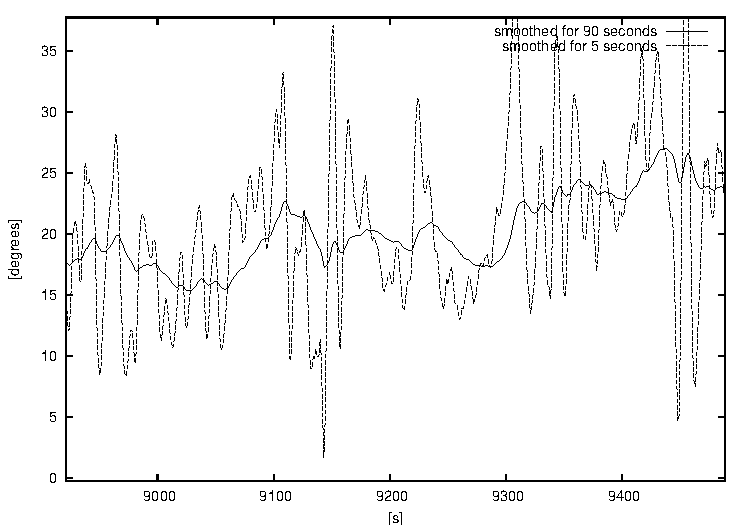
\includegraphics[width = 6.5 cm]{pics/paper_cleanwind.pdf}
 \caption{Differently filtered wind information}
 \label{fig:cleanwind}
\end{figure}

%
\subsection{Planning algorithm}
As explained earlier, \textit{Dijkstra}'s graph search is the basic algorithm
used to perform the path search. Starting at an initial grid-point, the algorithm expands over the whole field until the final grid-point has been reached. Every evaluated grid-point will be assigned a certain cost, a time estimate of how long it will take the boat to sail from the initial grid-point to the point that is currently being evaluated. The final optimal path is then determined by always following the neighbor with the lowest costs from the final to the initial grid-point. 

To be able to allocate costs for ship movements, i. e. moving from one grid-point to a neighbor, we work in 3 dimensions, with $x$ and $y$ for the geographic position
and $\theta$ for the heading of the boat at that position. To get sailable and
reasonable results, the following costs have been implemented additionally:
%
\begin{itemize}
\item Sailing-Time from start node
\item Estimated sailing time to the end node (heuristic)
\item Cost for heading changes
\item Cost for manoeuvres (tack and jibe)
\item Cost for offset from the straight connection between start and end node (tunnel cost).
\end{itemize}
%
\subsubsection{Grid compatible coordinate system}
To represent GPS points on a map, a coordinate transformation is necessary. Since we plan only for short distances ahead of us (local planning), we can use a very simplified transformation into meter coordinates 
\begin{equation}
\begin{array}{l}
 x = R_E \cdot \cos\left( \text{lat}\right) \cdot \dfrac{\pi}{180\, deg} \cdot \text{lon}\\
\\
 y = R_E \cdot\dfrac{\pi}{180\, deg}\cdot \text{lat}
\end{array}
\end{equation}
where $R_E$ is the earth radius, lon and lat the GPS coordinates in degrees. This transformation assumes a flat water surface \cite{stelzer2008}. In order to initialise the local map as small as possible, the algorithm places the origin as close as possible to either start or target coordinate. 
%
\subsubsection{Polar diagram}
In order to calculate the boat speed for a specific angle to the wind, a polar
diagram\footnote{In boating term, the polar diagram gives a boat velocity  as a
function of its  heading to the wind and the wind velocity} of \textsc{Avalon}
is needed.  Since creating a detailed diagram for our boat would require
constant wind and wave conditions over a long time, we created a polar diagram
based on existing diagrams for bigger vessels. Testing has shown that we get
reasonable results by restricting the sailable \textit{angle to the wind} to
the area between $45^o$ and $160^o$ (see figure \ref{fig:courses_to_wind}).
%
\subsubsection{Heading}
\hide{
% This is too much inmplementation dependent
We assume a 24 neighbour grid throughout this paper, which allows to have
sixteen different headings available for sailing. Another advantage of being
able to expand to the second but next neighbour-grid is the fact that it reduces
the number of way-points, since one grid node is skipped.
\subsubsection{Connectivity List}
In theory, every heading change is possible with a sailing boat. However, to
make the algorithm faster, we have constricted the biggest possible change of
heading to $90^o$. The areas that are not sailable due to the wind direction
are between $\pm45^o$ to wind direction for sailing upwind and $\pm160^o$ to
wind direction for sailing downwind (see figure \ref{fig:courses_to_wind}).
%
}
In order to limit the size of the 3D grid used in this paper, we use a
discretisation of the possible boat heading into 16 possible headings. In usual
2D grid-based path planning, transition from one cell to its 8 neighbours is
considered. This results in only 8 possible changes of orientation. By
considering a neighbourhood of 24 cells (8 cells around the starting cell, plus
16 cells one cell further), we can reach 16 different heading changes in one
transition. This leads to smoother paths and smaller number of way-points on the
final path.

We further reduce the computational complexity of the planner by considering
that the maximum change of heading in one transition is $90^o$. This
restriction is consistent with the experience of human skippers. 
%
\subsection{Cost Factors}
\subsubsection{General Costs}
The general aim of this algorithm is to find the shortest path for a sailing vessel to go from point $A$ to point $B$. The general cost we give for every movement is therefore \textit{sailing time to the next node}, calculated by equation \ref{eq:navi_timecost}. The speed solely depends on the angle to the wind and the wind speed. 
\begin{equation}
 \text{sailing time} = \frac{\text{distance to next node}}{\text{speed}} 
\label{eq:navi_timecost}
\end{equation}
\subsubsection{Heuristic Estimate}
The heuristic estimate is used to evaluate the remaining time to the goal.
According to \cite{lavalle2006}, the only constraint on the heuristic is that
it has to underestimate the real cost of the remaining path. For simplicity sake, the
heuristic returns the time it would take to sail to the goal at an exaggerated speed of 10 knots. More complicated options have been considered, but none of them provided well defined behaviour in all situations.

\subsubsection{Turning Cost}
To generate paths as smooth as possible, the algorithm places costs $C_{\text{new}}$ for heading changes, using a simple linear factor $f$ in equation
\begin{equation}
 C_{\text{new}} = f \cdot \vert \theta_{\text{curr}} - \theta_{\text{new}} \vert  
\label{eq:navi_turningcost}
\end{equation}
where $\theta_{\text{curr}}$ and $\theta_{\text{new}}$ are the respective headings. 
%
\subsubsection{Cost for Tack or Jibe}
By giving a certain cost for tack or jibe, we can indirectly control the number
of manoeuvres \textsc{Avalon} sails.  The principle is very simple, we check if
the sign of $(\theta_{\text{curr}} - \text{winddirection})$ and $(\theta_{\text{next}} -
\text{winddirection})$ is the same. If it is different, an additional cost will be
added to the total cost.
%
\subsubsection{Tunnel cost}
In order to favour paths that stay closer to the straight line path, we
allocate costs increasing with the distance from the direct connection of start
and target node. It has proved best to increase the cost only little for the
areas in the middle of the tunnel but increase it abruptly when closing in on
the borders. 
%
\subsubsection{Obstacle avoidance} 
To avoid islands and coastal regions, the algorithm gives extremely high costs
for passing prohibited terrain. To locate these areas, it parses information
from a map.\\
To avoid commercial ships on the Atlantic, \textsc{Avalon} can receive AIS
signals from most ships travelling over the Atlantic. Knowing ship speed,
direction and current position, our algorithm will place no-go areas around potential collision locations to make sure to bypass them.
%
% we had that already in chapter nav_strategy:
\hide{
\subsection{Trajectory tracker} \label{sec:skipper}
The trajectory tracker has mainly two important tasks:
\begin{itemize}
 \item Triggering the local planner
 \item Calculating a desired heading for the control system
\end{itemize}
\subsubsection{State machine}
To manage the different tasks, the trajectory tracker can switch between different states:
%
\paragraph{Standard Navigation}
If not approaching a target or buoy, this state generates headings for the control system, going from way-point to way-point.
If the wind changes more than $20$° or if the ship distances itself from the current trajectory for more than a predefined distance, a new calculation will be initiated. 
\paragraph{Goal Approach}
If approaching a target position, the trajectory tracker will always send a heading that is directing exactly towards that point.
\paragraph{Buoy Approach}
This is a state designed especially for short course racing. Due to regulations that always require a port-side surrounding of the regatta buoys, this state will - when approaching a buoy - always write a heading that will lead the boat around the buoy.
\paragraph{New Calculation}
In this state, the trajectory tracker manages and supervises the new calculation. After having checked that the new way-points have been stored, it switches back to \textit{Standard Navigation}
}
%
%
\subsection{Tests and Discussion}
\subsubsection{Testing environment}
Most tests and parameter optimization was done by visualising the generated
path on screen and discussing its quality. Figure \ref{fig:navi_path}
shows two calculated path examples, both having to pass an obstacle and dealing
with difficult wind direction like upwind and downwind. Analysis has shown that the addition of a tunnel cost is redundant since the heuristic estimate also favours paths that are close to the direct connection of {\em start} and {\em target} node. Although adding an artificial tunnel cost might not always result in optimal path solutions, we used the tunnel for safety reasons to make sure that the vessel never sails beyond predefined boundaries. 
\hide{
% In case of present obtacles, this is not always optimal.
\paragraph{Initial and final Heading}
Our initial motion was to set the current boat heading as $theta$ at the START
node. In case the TARGET was exactly in the opposite direction, the algorithm
then proposed a turn, which took about two to three way-points. Tests on the
water showed that this was not optimal at all and the manoeuvre cost us a lot of
time. We then set the START $theta$ directly towards the TARGET, which produced
much better results. One disadvantage is that the boat might sail away too far
from the starting point in case of long calculation time without receiving the
new heading. After calculation has finished, the trajectory tracker would then
notice the incoherence and trigger a new calculation. 
}

Another important and not yet solved problem is the final heading at the target
node that has to be known in order for \textit{Dijkstra} to start the search. At the
moment the algorithm chooses a final heading that is as close as possible to
the direct heading of a straight line from start to destination but always
differs at minimum $45^o$ from the wind direction. This usually produces good
results but it does not take obstacles into account which means that sometimes
an additional, unnecessary turn is produced. 

In practice, this issue will be solved by starting planning a new path before
completing the execution of the current one.


\begin{figure}[htb]
  \centering
  \subfloat[Upwind]{\label{fig:navi_upwind}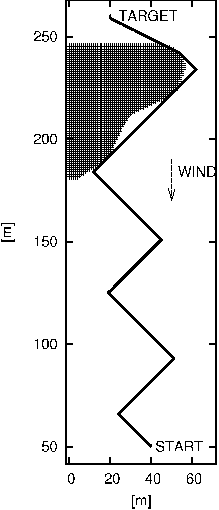
\includegraphics[width=2.7 cm]{pics/paper_kreuzen2.pdf}} 
  \hspace{1cm}
  \subfloat[Downwind]{\label{fig:navi_downwind}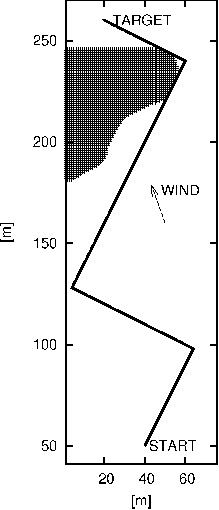
\includegraphics[width=2.7 cm]{pics/paper_downwind2.pdf}}
  \caption{Path examples for upwind and downwind sailing with obstacles}
  \label{fig:navi_path}
\end{figure}

\begin{figure}[htb]
\centering
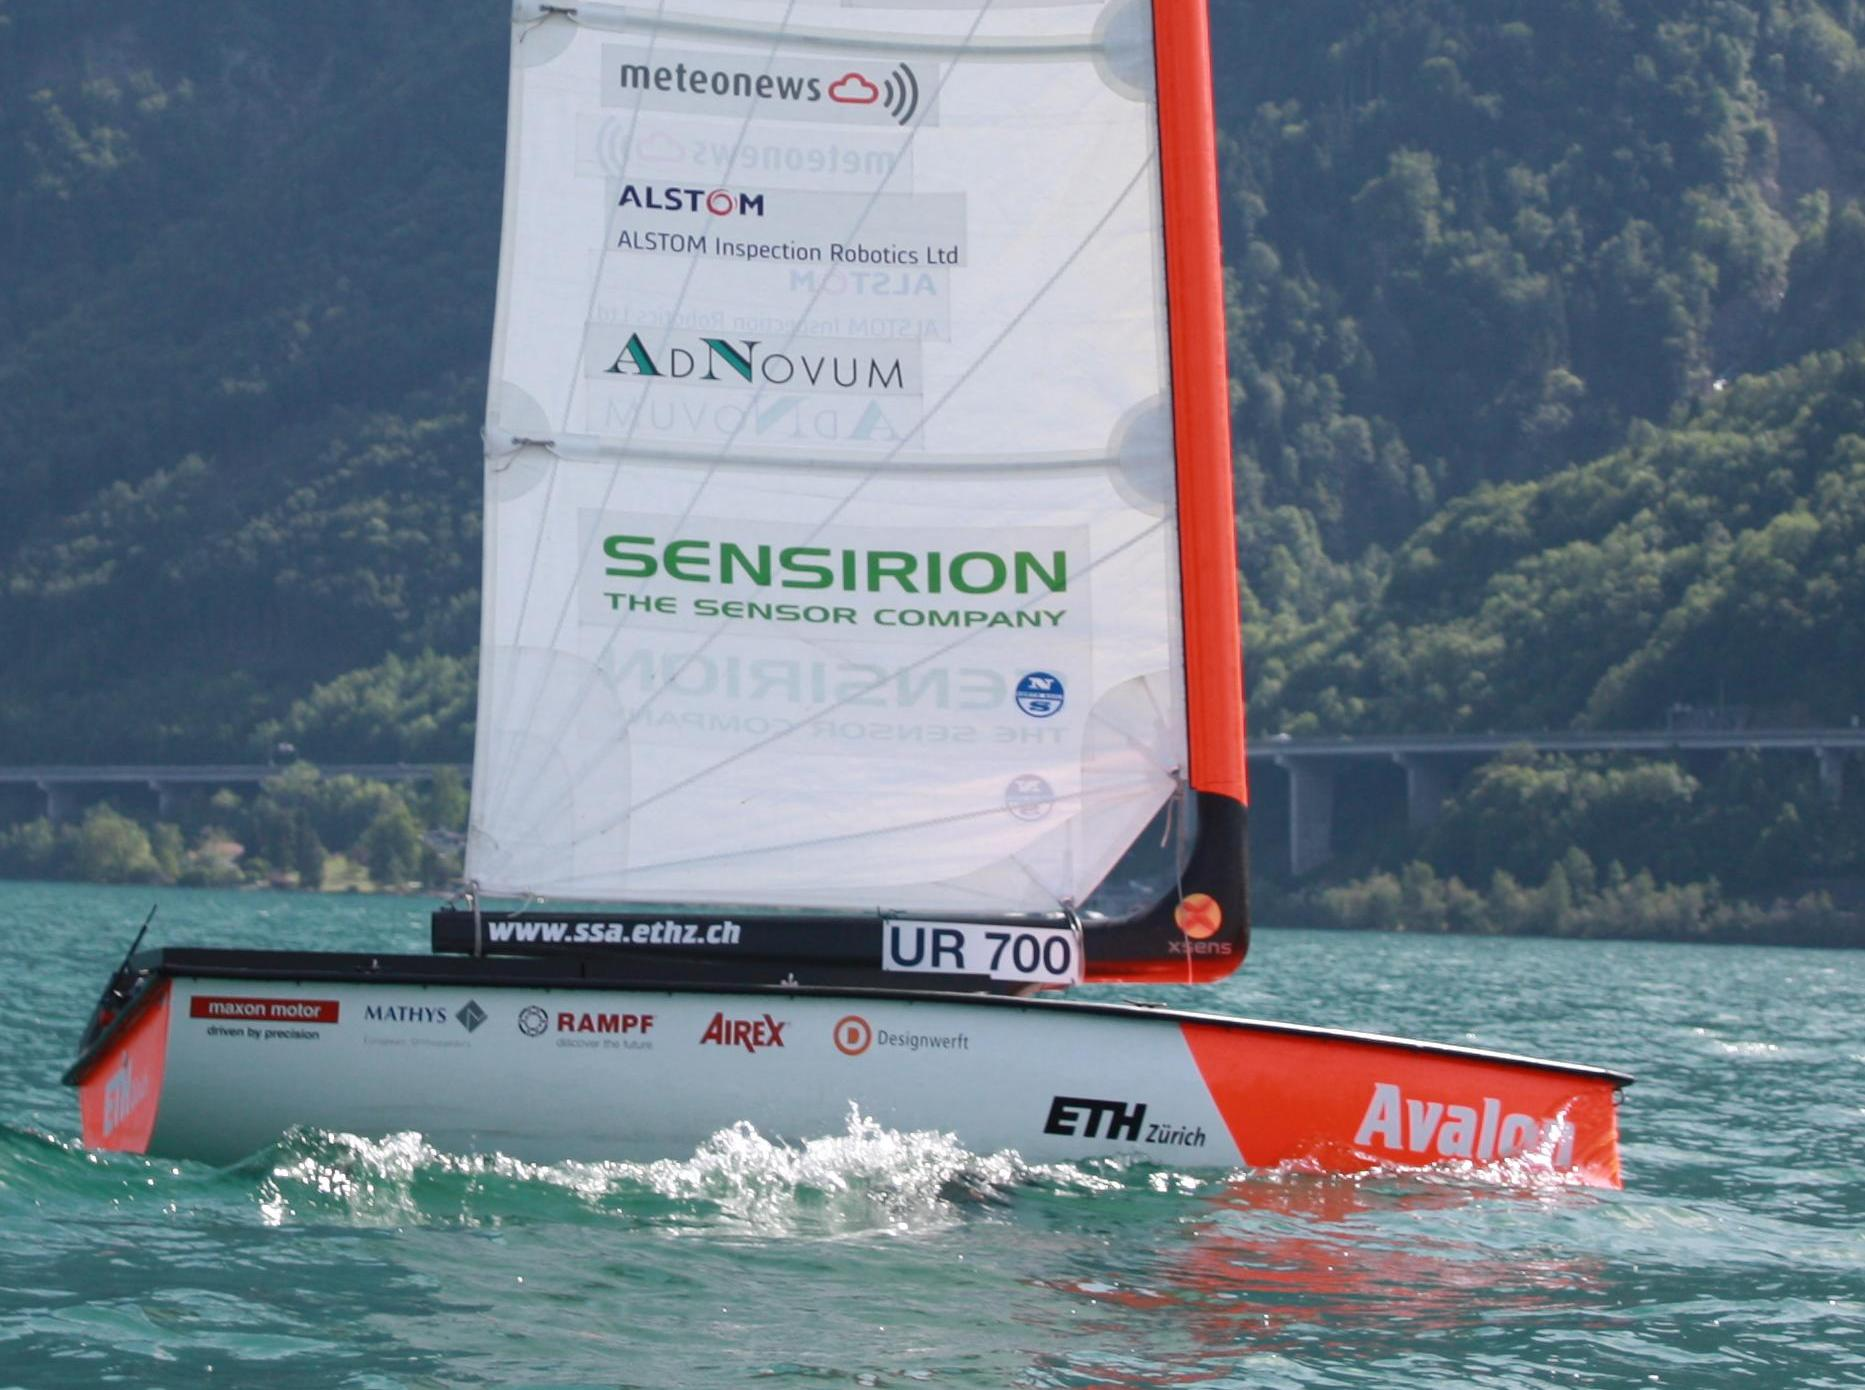
\includegraphics[width=0.75\columnwidth]{pics/IMG_0601_papercrop.jpeg}
\caption{Avalon during testing in high winds}
%\label{fig:avalon}
\end{figure}

\section{Conclusion and Outlook}
The proposed navigation and control software has been successfully implemented
in our autonomous sailboat \textsc{Avalon}. Several short-run tests both on
Swiss lakes and on the Atlantic Ocean have been carried out and have shown that the
described control and navigation system work. \textsc{Avalon} was exposed to
wind conditions ranging from almost 0 to 30 knots. The experimentally found
control parameters have proven to be well defined, keeping the vessel on course
even while sailing in rough sea states.

In very low wind speeds it was seen that the boat is able to sail much better
by itself than steered by us via remote control, because it is always aware of
the exact wind direction, even when human sailors hardly notice any wind at
all.

However, especially in reference to a possible crossing of the Atlantic Ocean,
several tests over a bigger period of time as well as longer distances have to
be performed in a next stage. 

By processing received AIS-signals, \textsc{Avalon} is able to identify other
ships in close proximity and therefore prevent collisions. However, small boats
that don't send position information cannot be recognized at this stage and
further research has to be done in identifying obstacles visually.   

Implementing a conventional and proved path planner like Dijkstra's for our
navigation system has proved well. Visually and analytically evaluated results
show that we achieve better solutions by taking the whole path into account
than by always optimising the heading at every current position. However, by
adding additional costs (like tunnel cost), optimal path solutions are not
always guaranteed.

Our goal for future work is to further optimise the software, especially
regarding energy consumption. For example a hysteresis could be added to the
sail tuner so that the sail does not constantly adapt to minor changes in wind
direction and speed. A further area of improvement could be in making use of
weather forecasts in the global navigation. For our boat this does not add much
value, because it is too slow to react to forecast weather changes.


% can use a bibliography generated by BibTeX as a .bbl file
% BibTeX documentation can be easily obtained at:
% http://www.ctan.org/tex-archive/biblio/bibtex/contrib/doc/
% The IEEEtran BibTeX style support page is at:
% http://www.michaelshell.org/tex/ieeetran/bibtex/
\bibliographystyle{IEEEtran}
\bibliography{IEEEabrv,ram_paper_ssa}

%

% Note that the a4paper option is mainly intended so that authors in
% countries using A4 can easily print to A4 and see how their papers will
% look in print - the typesetting of the document will not typically be
% affected with changes in paper size (but the bottom and side margins will).
% Use the testflow package mentioned above to verify correct handling of
% both paper sizes by the user's LaTeX system.
%
% Also note that the "draftcls" or "draftclsnofoot", not "draft", option
% should be used if it is desired that the figures are to be displayed in
% draft mode.
%
\documentclass[journal,final,letterpaper,twoside,twocolumn]{IEEEtran}
%\documentclass[journal,final,letterpaper,twoside,twocolumn]{IEEEtran}
% Add the compsoc option for Computer Society conferences.
%
% If IEEEtran.cls has not been installed into the LaTeX system files,
% manually specify the path to it like:
% \documentclass[conference]{../sty/IEEEtran}

\usepackage[utf8]{inputenc}        % Keybord settings


% Some very useful LaTeX packages include:
% (uncomment the ones you want to load)


% *** MISC UTILITY PACKAGES ***
%
%\usepackage{ifpdf}
% Heiko Oberdiek's ifpdf.sty is very useful if you need conditional
% compilation based on whether the output is pdf or dvi.
% usage:
% \ifpdf
%   % pdf code
% \else
%   % dvi code
% \fi
% The latest version of ifpdf.sty can be obtained from:
% http://www.ctan.org/tex-archive/macros/latex/contrib/oberdiek/
% Also, note that IEEEtran.cls V1.7 and later provides a builtin
% \ifCLASSINFOpdf conditional that works the same way.
% When switching from latex to pdflatex and vice-versa, the compiler may
% have to be run twice to clear warning/error messages.






% *** CITATION PACKAGES ***
%
\usepackage{cite}
\usepackage{textcomp}

% cite.sty was written by Donald Arseneau
% V1.6 and later of IEEEtran pre-defines the format of the cite.sty package
% \cite{} output to follow that of IEEE. Loading the cite package will
% result in citation numbers being automatically sorted and properly
% "compressed/ranged". e.g., [1], [9], [2], [7], [5], [6] without using
% cite.sty will become [1], [2], [5]--[7], [9] using cite.sty. cite.sty's
% \cite will automatically add leading space, if needed. Use cite.sty's
% noadjust option (cite.sty V3.8 and later) if you want to turn this off.
% cite.sty is already installed on most LaTeX systems. Be sure and use
% version 4.0 (2003-05-27) and later if using hyperref.sty. cite.sty does
% not currently provide for hyperlinked citations.
% The latest version can be obtained at:
% http://www.ctan.org/tex-archive/macros/latex/contrib/cite/
% The documentation is contained in the cite.sty file itself.






% *** GRAPHICS RELATED PACKAGES ***
%
\ifCLASSINFOpdf
  \usepackage[pdftex]{graphicx}
  % declare the path(s) where your graphic files are
  % \graphicspath{{../pdf/}{../jpeg/}}
  % and their extensions so you won't have to specify these with
  % every instance of \includegraphics
  % \DeclareGraphicsExtensions{.pdf,.jpeg,.png}
\else
  % or other class option (dvipsone, dvipdf, if not using dvips). graphicx
  % will default to the driver specified in the system graphics.cfg if no
  % driver is specified.
 \usepackage[dvips]{graphicx}
  % declare the path(s) where your graphic files are
  % \graphicspath{{../eps/}}
  % and their extensions so you won't have to specify these with
  % every instance of \includegraphics
  % \DeclareGraphicsExtensions{.eps}
\fi
% graphicx was written by David Carlisle and Sebastian Rahtz. It is
% required if you want graphics, photos, etc. graphicx.sty is already
% installed on most LaTeX systems. The latest version and documentation can
% be obtained at:
% http://www.ctan.org/tex-archive/macros/latex/required/graphics/
% Another good source of documentation is "Using Imported Graphics in
% LaTeX2e" by Keith Reckdahl which can be found as epslatex.ps or
% epslatex.pdf at: http://www.ctan.org/tex-archive/info/
%
% latex, and pdflatex in dvi mode, support graphics in encapsulated
% postscript (.eps) format. pdflatex in pdf mode supports graphics
% in .pdf, .jpeg, .png and .mps (metapost) formats. Users should ensure
% that all non-photo figures use a vector format (.eps, .pdf, .mps) and
% not a bitmapped formats (.jpeg, .png). IEEE frowns on bitmapped formats
% which can result in "jaggedy"/blurry rendering of lines and letters as
% well as large increases in file sizes.
%
% You can find documentation about the pdfTeX application at:
% http://www.tug.org/applications/pdftex





% *** MATH PACKAGES ***
%
\usepackage[cmex10]{amsmath}
% A popular package from the American Mathematical Society that provides
% many useful and powerful commands for dealing with mathematics. If using
% it, be sure to load this package with the cmex10 option to ensure that
% only type 1 fonts will utilized at all point sizes. Without this option,
% it is possible that some math symbols, particularly those within
% footnotes, will be rendered in bitmap form which will result in a
% document that can not be IEEE Xplore compliant!
%
% Also, note that the amsmath package sets \interdisplaylinepenalty to 10000
% thus preventing page breaks from occurring within multiline equations. Use:
%\interdisplaylinepenalty=2500
% after loading amsmath to restore such page breaks as IEEEtran.cls normally
% does. amsmath.sty is already installed on most LaTeX systems. The latest
% version and documentation can be obtained at:
% http://www.ctan.org/tex-archive/macros/latex/required/amslatex/math/





% *** SPECIALIZED LIST PACKAGES ***
%
%\usepackage{algorithmic}
% algorithmic.sty was written by Peter Williams and Rogerio Brito.
% This package provides an algorithmic environment fo describing algorithms.
% You can use the algorithmic environment in-text or within a figure
% environment to provide for a floating algorithm. Do NOT use the algorithm
% floating environment provided by algorithm.sty (by the same authors) or
% algorithm2e.sty (by Christophe Fiorio) as IEEE does not use dedicated
% algorithm float types and packages that provide these will not provide
% correct IEEE style captions. The latest version and documentation of
% algorithmic.sty can be obtained at:
% http://www.ctan.org/tex-archive/macros/latex/contrib/algorithms/
% There is also a support site at:
% http://algorithms.berlios.de/index.html
% Also of interest may be the (relatively newer and more customizable)
% algorithmicx.sty package by Szasz Janos:
% http://www.ctan.org/tex-archive/macros/latex/contrib/algorithmicx/




% *** ALIGNMENT PACKAGES ***
%
%\usepackage{array}
% Frank Mittelbach's and David Carlisle's array.sty patches and improves
% the standard LaTeX2e array and tabular environments to provide better
% appearance and additional user controls. As the default LaTeX2e table
% generation code is lacking to the point of almost being broken with
% respect to the quality of the end results, all users are strongly
% advised to use an enhanced (at the very least that provided by array.sty)
% set of table tools. array.sty is already installed on most systems. The
% latest version and documentation can be obtained at:
% http://www.ctan.org/tex-archive/macros/latex/required/tools/


%\usepackage{mdwmath}
%\usepackage{mdwtab}
% Also highly recommended is Mark Wooding's extremely powerful MDW tools,
% especially mdwmath.sty and mdwtab.sty which are used to format equations
% and tables, respectively. The MDWtools set is already installed on most
% LaTeX systems. The lastest version and documentation is available at:
% http://www.ctan.org/tex-archive/macros/latex/contrib/mdwtools/


% IEEEtran contains the IEEEeqnarray family of commands that can be used to
% generate multiline equations as well as matrices, tables, etc., of high
% quality.


%\usepackage{eqparbox}
% Also of notable interest is Scott Pakin's eqparbox package for creating
% (automatically sized) equal width boxes - aka "natural width parboxes".
% Available at:
% http://www.ctan.org/tex-archive/macros/latex/contrib/eqparbox/





% *** SUBFIGURE PACKAGES ***
%\usepackage[tight,footnotesize]{subfig}
% subfigure.sty was written by Steven Douglas Cochran. This package makes it
% easy to put subfigures in your figures. e.g., "Figure 1a and 1b". For IEEE
% work, it is a good idea to load it with the tight package option to reduce
% the amount of white space around the subfigures. subfigure.sty is already
% installed on most LaTeX systems. The latest version and documentation can
% be obtained at:
% http://www.ctan.org/tex-archive/obsolete/macros/latex/contrib/subfigure/
% subfigure.sty has been superceeded by subfig.sty.



\usepackage[caption=false]{caption}
\usepackage[font=footnotesize]{subfig}
% subfig.sty, also written by Steven Douglas Cochran, is the modern
% replacement for subfigure.sty. However, subfig.sty requires and
% automatically loads Axel Sommerfeldt's caption.sty which will override
% IEEEtran.cls handling of captions and this will result in nonIEEE style
% figure/table captions. To prevent this problem, be sure and preload
% caption.sty with its "caption=false" package option. This is will preserve
% IEEEtran.cls handing of captions. Version 1.3 (2005/06/28) and later
% (recommended due to many improvements over 1.2) of subfig.sty supports
% the caption=false option directly:
%\usepackage[caption=false,font=footnotesize]{subfig}
%
% The latest version and documentation can be obtained at:
% http://www.ctan.org/tex-archive/macros/latex/contrib/subfig/
% The latest version and documentation of caption.sty can be obtained at:
% http://www.ctan.org/tex-archive/macros/latex/contrib/caption/




% *** FLOAT PACKAGES ***
%
%\usepackage{fixltx2e}
% fixltx2e, the successor to the earlier fix2col.sty, was written by
% Frank Mittelbach and David Carlisle. This package corrects a few problems
% in the LaTeX2e kernel, the most notable of which is that in current
% LaTeX2e releases, the ordering of single and double column floats is not
% guaranteed to be preserved. Thus, an unpatched LaTeX2e can allow a
% single column figure to be placed prior to an earlier double column
% figure. The latest version and documentation can be found at:
% http://www.ctan.org/tex-archive/macros/latex/base/



%\usepackage{stfloats}
% stfloats.sty was written by Sigitas Tolusis. This package gives LaTeX2e
% the ability to do double column floats at the bottom of the page as well
% as the top. (e.g., "\begin{figure*}[!b]" is not normally possible in
% LaTeX2e). It also provides a command:
%\fnbelowfloat
% to enable the placement of footnotes below bottom floats (the standard
% LaTeX2e kernel puts them above bottom floats). This is an invasive package
% which rewrites many portions of the LaTeX2e float routines. It may not work
% with other packages that modify the LaTeX2e float routines. The latest
% version and documentation can be obtained at:
% http://www.ctan.org/tex-archive/macros/latex/contrib/sttools/
% Documentation is contained in the stfloats.sty comments as well as in the
% presfull.pdf file. Do not use the stfloats baselinefloat ability as IEEE
% does not allow \baselineskip to stretch. Authors submitting work to the
% IEEE should note that IEEE rarely uses double column equations and
% that authors should try to avoid such use. Do not be tempted to use the
% cuted.sty or midfloat.sty packages (also by Sigitas Tolusis) as IEEE does
% not format its papers in such ways.




% *** PDF, URL AND HYPERLINK PACKAGES ***
%
%\usepackage{url}
% url.sty was written by Donald Arseneau. It provides better support for
% handling and breaking URLs. url.sty is already installed on most LaTeX
% systems. The latest version can be obtained at:
% http://www.ctan.org/tex-archive/macros/latex/contrib/misc/
% Read the url.sty source comments for usage information. Basically,
% \url{my_url_here}.





% *** Do not adjust lengths that control margins, column widths, etc. ***
% *** Do not use packages that alter fonts (such as pslatex).         ***
% There should be no need to do such things with IEEEtran.cls V1.6 and later.
% (Unless specifically asked to do so by the journal or conference you plan
% to submit to, of course. )


% correct bad hyphenation here
\hyphenation{op-tical net-works semi-conduc-tor middle-ware}

\newcommand{\hide}[1]{}
\begin{document}
%
% paper title
% can use linebreaks \\ within to get better formatting as desired
\title{Navigation Strategy and Trajectory Following Controller for an Autonomous Sailing Vessel}



% author names and affiliations
% use a multiple column layout for up to three different
% affiliations



%\author{

%\IEEEauthorblockN{Sebastian Boehl\IEEEauthorrefmark{1}}

%\and

%\IEEEauthorblockN{Lian P. Giger}
%\IEEEauthorblockA{ETH\\Federal Institute of Technology\\
%Zurich, Switzerland\\
%Email: ligiger@student.ethz.ch}

%\and

%\IEEEauthorblockN{Stefan Wismer} \IEEEauthorblockA{ETH Zurich}}

% conference papers do not typically use \thanks and this command
% is locked out in conference mode. If really needed, such as for
% the acknowledgment of grants, issue a \IEEEoverridecommandlockouts
% after \documentclass

% for over three affiliations, or if they all won't fit within the width
% of the page, use this alternative format:
%
\author{\IEEEauthorblockN{Hendrik Erckens ({\small corresponding author}), Gion-Andri Büsser,\\Dr. C\'{e}dric Pradalier, Prof Dr. Roland Y. Siegwart\\ \IEEEauthorblockA{Autonomous Systems Lab, Swiss Federal
Institute of Technology (ETH) Zurich\\Leonhardstrasse 25, 8092 Zurich, Switzerland \\
E-mail: herckens@student.ethz.ch}}}

% use for special paper notices
%\IEEEspecialpapernotice{(Invited Paper)}

% make the title area
\maketitle
\begin{abstract}
%\boldmath
This paper describes the design and implementation of a navigation and control
system for the autonomous sailing
vessel {\sc Avalon}. This boat, designed for participating in the {\sc
Microtransat}, is engineered to autonomously cross the Atlantic Ocean. We
present here a specially robust mechanical design and the navigation software
that will plan an optimal navigation course and efficiently control the boat on
this course. The path planner uses an A* algorithm to generate the fastest path
to a given destination. It is able to avoid both static and dynamic obstacles.
By using a given polar diagram and measured wind data, it takes into account
manoeuvrability constraints of a sailboat. The control system takes care of
rudder and sail in order to follow a given heading while optimising speed.
Additionally, the system is capable of automatically conducting manoeuvres such
as tack and jibe. 
At the time of this writing, {\sc Avalon} and its software systems have been
successfully tested more than two weeks in short deployments lasting several
hours with winds ranging from 0 up to 30 knots. 
\end{abstract}
% IEEEtran.cls defaults to using nonbold math in the Abstract.
% This preserves the distinction between vectors and scalars. However,
% if the conference you are submitting to favors bold math in the abstract,
% then you can use LaTeX's standard command \boldmath at the very start
% of the abstract to achieve this. Many IEEE journals/conferences frown on
% math in the abstract anyway.
%
% no keywords
%
% For peer review papers, you can put extra information on the cover
% page as needed:
% \ifCLASSOPTIONpeerreview
% \begin{center} \bfseries EDICS Category: 3-BBND \end{center}
% \fi
%
% For peerreview papers, this IEEEtran command inserts a page break and
% creates the second title. It will be ignored for other modes.
% \IEEEpeerreviewmaketitle
%
\section{Introduction}
%\subsection{General Objectives for building an autonomous sailboat}
This paper introduces the autonomous sailboat \textsc{Avalon} as seen in figure
\ref{fig:avalon}. The general objective for building an autonomous sailing
vessel is to further research and development in the area of unmanned,
autonomous robotic vehicles that are exposed to heavy environmental conditions
such as the Atlantic Ocean. It has been established that there is a demand for
autonomous sailboats to be used for ocean sampling and surveillance
\cite{cruz:ase} but also for the implementation of this type of software in
manned sailing vessels. Either by passively proposing optimal sailing routes or
by actively supporting the sailor in dangerous situations by piloting the sail
or rudders, an integrated autonomous sailing system could back up and
facilitate a lot of situations. For example, if a single hand sailor falls over
board, the system could detect this incident and automatically execute a Man
Over Board manoeuvre.

\subsection{Our Goals and Objectives for this Work}
Our boat \textsc{Avalon} was designed to compete in the \textsc{Microtransat}
Challenge and thus has to withstand the harsh conditions on the Atlantic Ocean.

The goal of this paper is to present a software that is
capable of calculating the optimal path to reach a given destination as quickly
as possible, and the design of a controller able to safely and efficiently
guide the sailboat along the calculated path, taking into account the current
environmental conditions, such as wind speed.
\hide{Furthermore, it should be able to respond to a possible shortness of
energy by adjusting the control parameters or changing the mode of sailing.}


\subsection{Review of Existing Autonomous Sailing Boats}
An autonomous sailboat has to be capable of sailing without human intervention.
That means, that all tasks that are normally carried out by the sailor on a
conventional sailboat have to be done autonomously. That involves navigation
as well as working the rudder and sail in order to steer the defined course.
Other autonomous sailboats have been developed mostly by \textsc{Microtransat}
participants \cite{briere2008iar}, \cite{stelzer2008}, \cite{alves:fas},
\cite{sauze2008dcs}, but also commercially usable products \cite{harborwing}
have been built. In contrast to most of the existing work, we use a path
planner to avoid obstacles. Additionally, our controller switches between many
different modes of sailing, in order to make better use of wind shifts.

\section{A Boat Designed for Survival}
To provide an insight into the platform that was used to implement the proposed
software, this section summarises some details about the main components of
{\sc Avalon}. The mechanical system was more comprehensively described in
\cite{giger2009}. Table \ref{tab:avalon_data} shows the major technical details
of {\sc Avalon}.
\begin{figure}[b!]
\centering
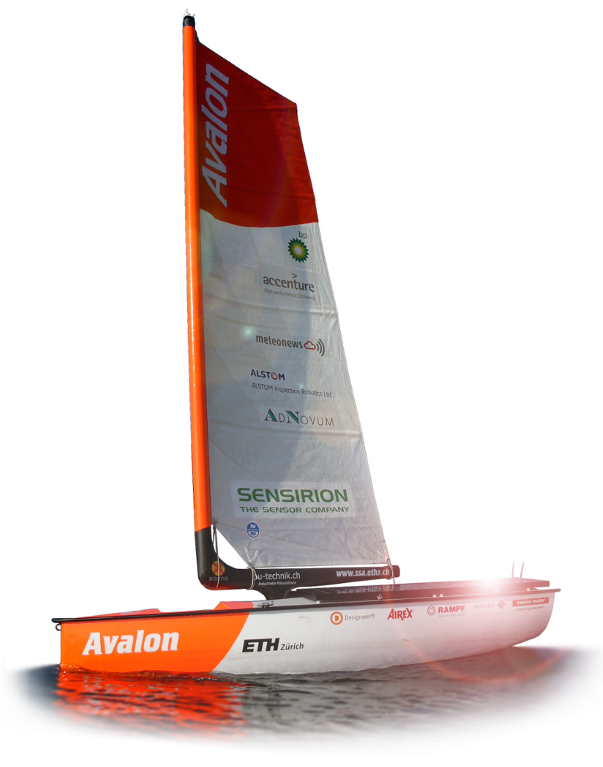
\includegraphics[height=0.8\columnwidth]{pics/avalon.png}
\caption{Avalon ready to sail on the lake of Z\"urich}
\label{fig:avalon}
\end{figure}

\subsection{Rig}
The rigging system is one of the most important parts of the whole
assembly. A defect in its structure will inevitably cause the whole project to
fail. The following aspects were considered for the design:
\begin{itemize}
\item High loads and forces on the mechanical structures due to
strong winds and heavy weather conditions.
\item Highest demands on reliability. There is no chance to
repair anything throughout the journey.
\item Preferably efficient force transmission from the actuator to the sail in order to save as much energy as
possible
\end{itemize}

During the design phase it turned out that a balanced rig prevails over a
conventional rig.
\hide{
The balanced rig is much more efficient regarding energy
consumption than any other conventional rig. The force needed to position the
sail is reduced by over 50\% due to the balanced distribution of
the sail load. Furthermore, }\textsc{Avalon}'s rig does not use any ropes
that could generate knots and jams. It is pivoted on a central
bearing without shrouds and stays. The result is a simple and reliable construction.
%
\subsection{Hull}
\hide{The hull design is based on form parameters, e.g. length, draft and
beam. Parameters were used as input data for B-spline curves and
surfaces. Instead of modifying those curves and surfaces, we used
constrained optimisation algorithms to generate the geometry. The algorithm
minimises a target function, which is defined so that a certain combination of
parameters results in a desired hull shape.}

The hull was designed using the CAE software \textsc{FRIENDSHIP-Framework} and
was laminated inside a female mold using glass fibre
sandwich. Epoxide resin was sucked into dry glass fibre material by
vacuum in a so called \textit{Infusion Process}. Compared to
conventional laminating, this method is much cleaner and more
convenient.

%---------------------------------------------------------
%basicdata: AVALON
%---------------------------------------------------------
\begin{table}[htb]

    \begin{center}
     \caption{Technical Data of \textsc{Avalon}}
	\label{tab:avalon_data}
%        \begin{tabular}[h!]{p{0.15\textwidth}| p{0.2\textwidth}| p{0.05\textwidth}}
        \begin{tabular}[htb]{l|l|l}
            \hline
            \emph{Variable}    &   \emph{Description} &   \emph{Value}\\ \hline\hline
            $L_{OA}$    &   Length over all	& $3.95\,m$\\
            $B_{max}$   &   Maximal beam	& $0.7\,m$\\
            $T$         &   Draft without keel  & $0.25\,m$\\
            $D_{max}$	&   Draft over all	& $2\,m$\\
            $H_{rigg}$	&   Height of the rigg  & $5.7\,m$\\
            $A_{sail}$	&   Total sail area     & $8.4\,m^2$\\
            $\nabla$    &   Submerged volume    & $0.44\,m^3$\\
            \hline
        \end{tabular}
    \end{center}
\end{table}


\begin{figure}[htb]
\centering
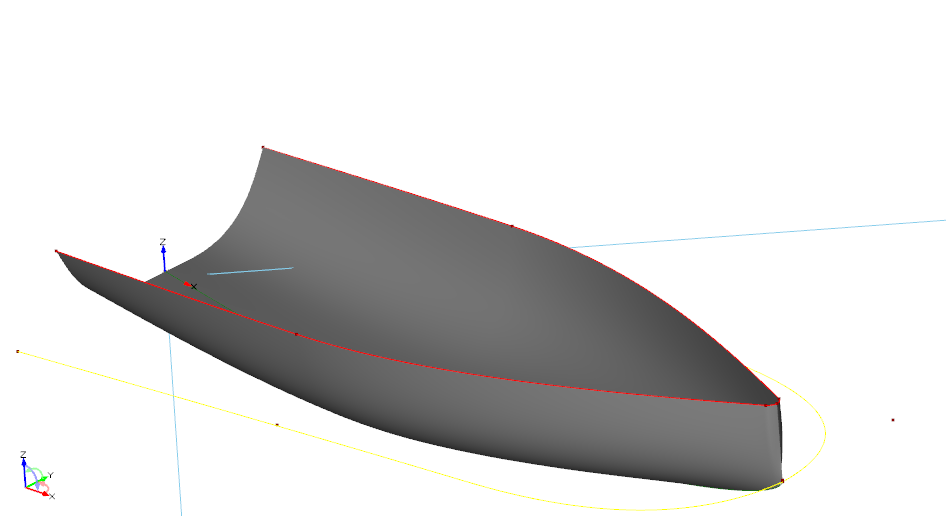
\includegraphics[width=0.37\textwidth]{pics/hull.png}
\caption{Hull} \label{fig:hull}
\end{figure}

%
\subsection{Keel and Rudder}
\subsubsection{Keel}
In order to achieve a sufficient righting moment and stability
during heavy weather situations, {\sc Avalon}'s keel with a draft of
two meters consists of a slim fin with a 160\,kg ballast bulb.

The fin and parts of the bulb were made of high-modulus carbon fibre
in precisely milled polyurethane female molds. After hardening and
tempering, the bulb was filled with lead and the two halves were
glued together.

\begin{figure}[htb]
\centering
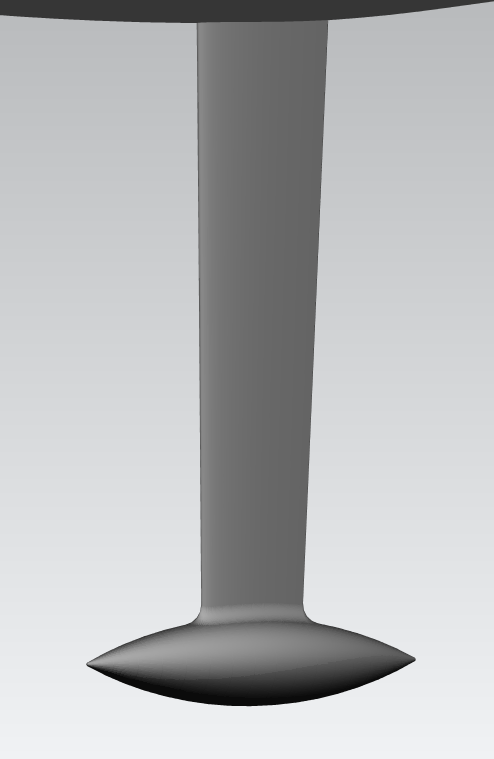
\includegraphics[width=2.7cm]{pics/keel.png}\hfill
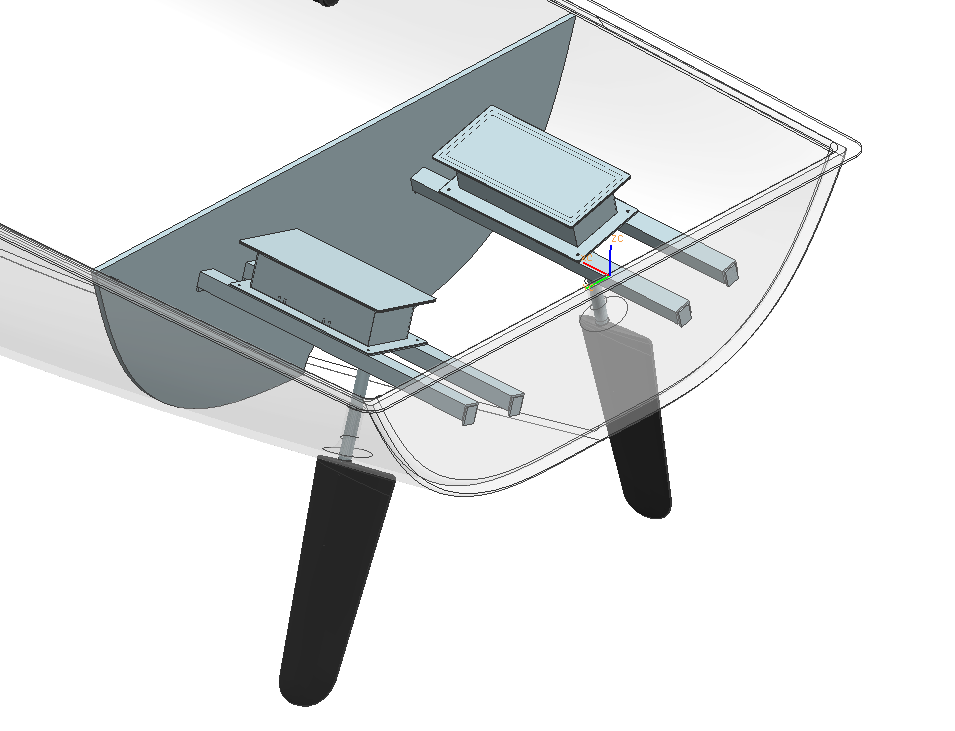
\includegraphics[width=4.5cm]{pics/rudder.png}
% \caption{Twin rudder system} \label{fig:cadrudder}
\caption{Keel with fin and ballast bulb (left), Twin rudder system (right)} \label{fig:cadkeel}
\end{figure}

\subsubsection{Rudder}
A twin-rudder system was selected for {\sc Avalon} to make sure to
have sufficient steering effect in every sailing situation. Angular
mounted twin-rudders provide better control at high
heeling angles compared to single rudders.

Assembled inside the hull, the rudder actuators are well sealed and
protected against water and humidity.

% \begin{figure}[htb]
% \centering
% 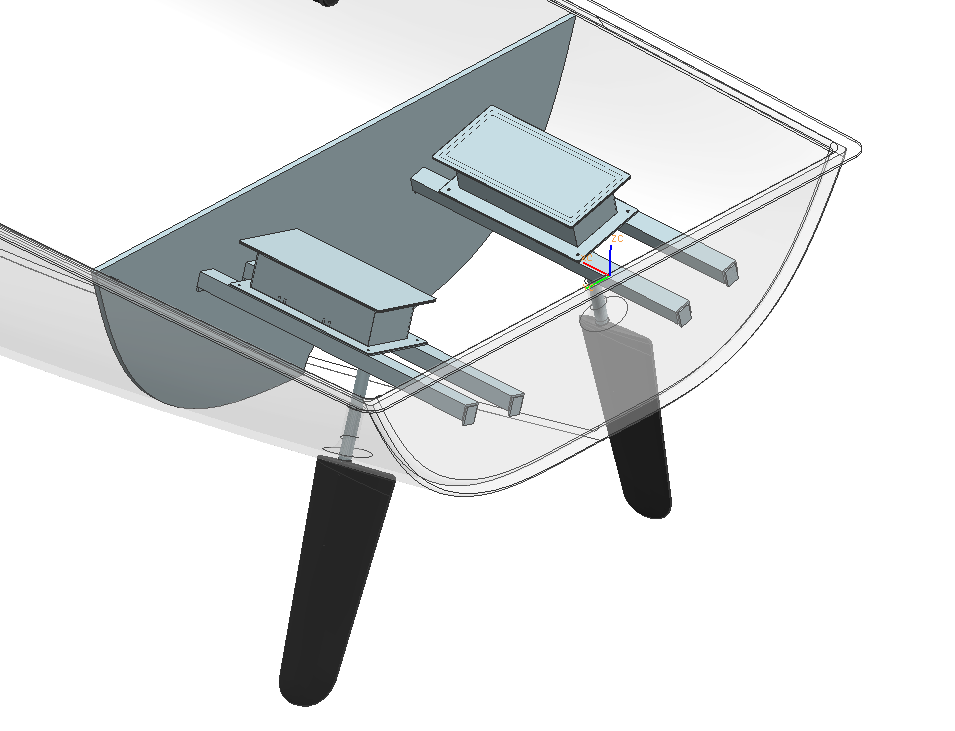
\includegraphics[width=4cm]{pics/rudder.png}
% \caption{Twin rudder system} \label{fig:cadrudder}
% \end{figure}
%
\subsection{Power Supply}
The main power supply is realised through two square meters of solar panels providing
a total of 360\,Wp. The collected energy is stored in four lithium-manganese
batteries. Each battery consists of 70 single cells and has a capacity of
600\,Wh at a nominal voltage of 25.2\,volts. Lithium-manganese batteries were
chosen mainly because of their weight but also because they are fairly safe to
use.

For back-up power, the boat has a direct-methanol fuel cell on
board. This fuel cell is automatically activated when the voltage
drops under a certain value, the \emph{switch on} voltage. It then
charges the batteries until the \emph{switch off} voltage is
reached. In theory, the solar cells provide enough power for the
boat's systems. The fuel cell only serves in case of enduring bad
weather  or other unforeseeable circumstances.



\section{Navigation Stategy}
This chapter will give a general overview of the software developed for
\textsc{Avalon} and discuss the interaction between control system and path
planner. Sections \ref{sec:sailor} and \ref{sec:navigator} will then go further
into details of the actual controller and path planner respectively.

The core hardware part and the brain of the system on the sailing vessel is the
main computer MPC21 from {\sc DigitalLogic}, a 500\,MHz device with 1024\,MB
RAM and a compact flash hard-drive. The device has an average power consumption
of about 8\,watts, the protection of a metal housing and a total weight of less
than 1\,kg.
% \begin{figure}[htb]
% \centering
% 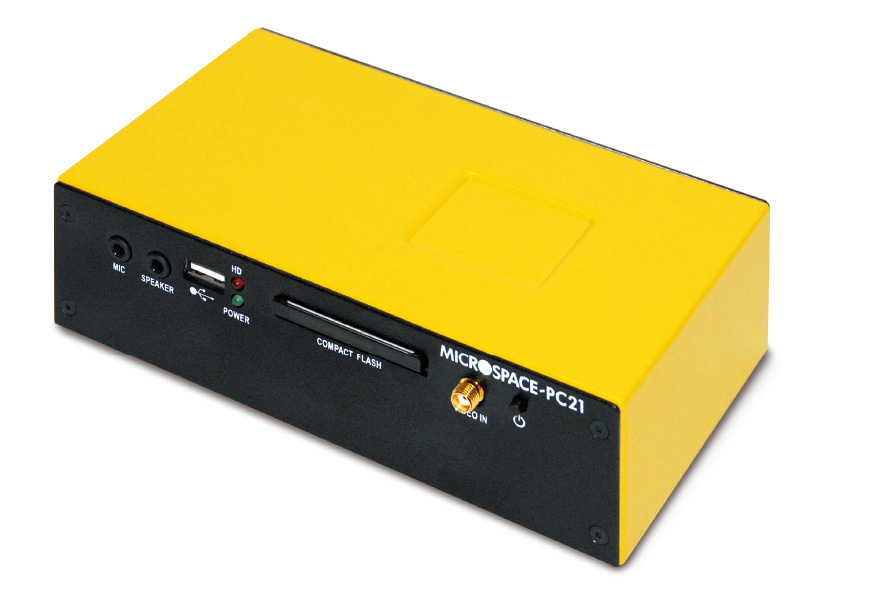
\includegraphics[height=4.0cm]{pics/RE_MPC21.png}\label{fig:mainpc}
% \caption{Main PC and brain of {\sc Avalon}\cite{digitallogic}}
% \end{figure}
%
The base of the entire software structure is the middleware DDX\cite{ddxpaper}
that runs on a Linux Operating System. This software manages a shared memory
called the Store and thus provides a means of communication between individual
programs that all run in parallel (see figure \ref{fig:ddx}). 

Sensor drivers will collect data from the specific sensors (see section
\ref{sec:sensors}) and store it in the DDX Store, from where it can be accessed
by the control and path planning programs.
% 
% A distinct advantage of DDX is the modular software structure. If ever a
% program crashes, it can be restarted without interrupting the other processes.
The different subprograms used on \textsc{Avalon} are depicted in figure
\ref{fig:ddx}.

\begin{figure}[htb]
\centering
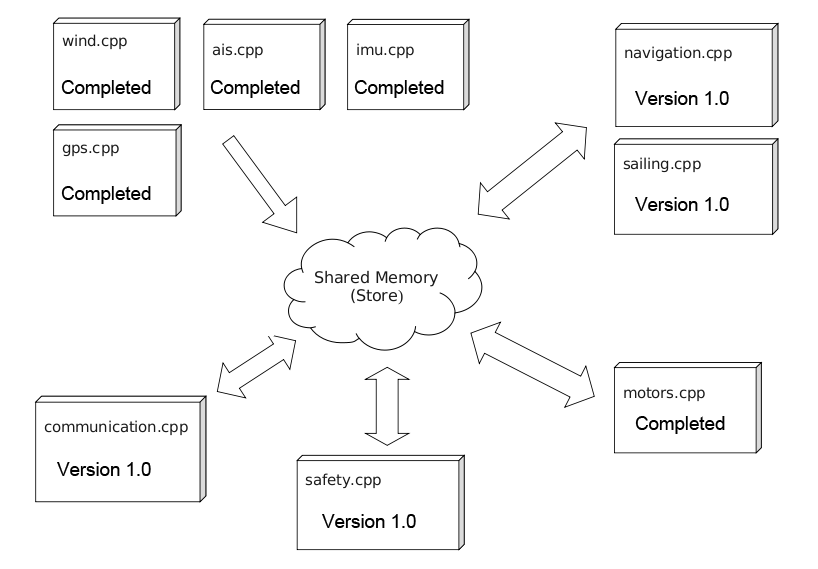
\includegraphics[height=5.5cm]{pics/RE_ddxplain.png}
\caption{Software organisation} \label{fig:ddx}
\end{figure}

%
%
\subsection{Sensors} \label{sec:sensors}
All desired information such as position, heading or speed are measured by
several sensors located all over the boat. To get a fully controllable system,
data is collected from the following sensors:
%
%\begin{description}[\IEEEsetlabelwidth{Wind}\IEEEusemathlabelsep]
%\item[\textbf{GPS}] 
\subsubsection{GPS \& IMU} 
%Provides position, heading and speed. The sensor's antenna is mounted on top of the mast. The electronic unit is located in the hull.
%\item[\textbf{IMU}]
The localization of the boat is performed by an \textit{Inertial Measurement
Unit} (by \textsc{X-Sens}) that is combined with a GPS receiver. Using the
accelerations in all 6 degrees of freedom and a high update rate of 120 Hz,
occasional deviations of the GPS-data will automatically be smoothed out. The
system therefore produces highly accurate positioning.
%
%\item[\textbf{Wind}]
\subsubsection{Wind} Mounted on top of the mast, the wind-sensor provides wind
speed and direction. {\sc Avalon} has an ultrasonic wind-sensor that promises
less mechanical failure than a conventional sensor with a turning wheel. The
sensor by Danish company \textsc{Deif} is IP-66 approved and connected to the
main computer via a RS-485 interface.
%\item[\textbf{AIS}]
\subsubsection{AIS} This Sensor receives data such as position and velocity
from other boats via VHF. The AIS system is an additional means of perception
that ensures that collisions with large commercial ships are avoided.
%\end{description}
%
\subsection{Navigation Management} \label{sec:skipper}
The overall navigation management is being performed by a program further
referred to as trajectory tracker. It's two main tasks are to trigger the local
planner of the path planning algorithm (see section \ref{sec:navigator}) and to
extract from a planned path a sailable boat heading that can be followed by the
controller (see section \ref{sec:sailor}).

The program keeps track of the boat's location as well as it's environment. In
case of predefined emergency cases, it is able to set new destination coordinates.

Having a state machine architecture, the trajectory tracker can switch between
the following states:
%
\subsubsection{Standard Navigation}
If not approaching a target\hide{ or buoy}, this state generates headings for the
control system, going from way-point to way-point. If the wind changes more than $20$°
or if the ship distances itself from the current trajectory for more than a
predefined distance, a new calculation will be initiated. 
\subsubsection{Goal Approach}
If approaching a target position, the trajectory tracker will always send a
heading that is directing exactly towards that point.
\hide{\subsubsection{Buoy Approach}
This is a state designed especially for short course racing. Due to regulations
that always require a port-side surrounding of the regatta buoys, this state
will - when approaching a buoy - always write a heading that will lead the boat
around the buoy.}
\subsubsection{New Calculation}
In this state, the trajectory tracker manages and supervises the new
calculation. After having checked that the new way-points have been stored, it
switches back to \textit{Standard Navigation}
%
%

\section{Control System}\label{sec:sailor}
\subsection{Objectives}
This section describes the design of a controller that is capable of robustly
steering a sailboat along a predefined course while always setting the sail to
the optimal angle to the wind in order to generate as much driving force as
possible. For that, it also has to be able to conduct manoeuvres such as tack
and jibe. At the same time, the controller should take into account the
changing environmental conditions, such as wind speed and direction and react
accordingly. Furthermore, since the path planner (section \ref{sec:navigator})
calculates a global trajectory and relies on the control system to follow this
course, the control system has to compensate for drift.
%
\subsection{Existing Works}
There are various systems available that assist a sailor in steering a
sailboat. Most of these are commercially available autopilots, that operate
either with a built in magnetic compass or with a wind vane
\cite{hochseeportverband1958s}. These systems are finished products, that have
been used for many years and are very robust and reliable. We did not use
commercial products, mainly because of interfacing issues. Autopilots are
designed for a human sailor on board who does the navigation and has to tune
the sails. Although some of the systems are even able to perform tacks and
jibes, the manoeuvre has to be confirmed by the human sailor pressing a button
on the autopilot's control panel. Since the software integrated in commercial
autopilots is typically closed source, this problem cannot be solved by simply
reprogramming the device. Furthermore, most autopilots only control the rudder,
so we would still have to figure out a way to tune the sail.

Apart from the commercial products, there are also several scientific works
regarding control systems for autonomous sailboats, most of them also by
participants in the \textsc{Microtransat}. Developments reach from a fuzzy
logic controller for both rudder and sail \cite{stelzerFuzzy}, over an LQG
controller based on a non-linear 3 degrees of freedom (DOF) model
\cite{elkaim:ska}, up to a complex self learning AI system that has been
successfully tested on an Open60 racing yacht. Our work is mainly influenced by
Briere \cite{briere2008iar}, who describes a simple controller based on a state
machine.
%
\subsection{System Modelling} In order to design a robust controller and
identify parameters in a controlled environment, a simulator is very helpful.
Although there are several sailing simulators available, most of them are made
for gaming. Rather than having an interface that allows them to be steered by a
self-developed control system, they are meant to be operated by hand. For this
reason we implemented a simulator in Matlab/Simulink.

To gain a general system that could later be extended with boat/wave
interaction, the boat was modelled as a rigid body with full 6 DOF. The system
has 12 state variables: 3 for position, 3 for attitude, 3 for velocity and 3 for
turning rates.  Inputs to the plant are rudder angle
$\gamma_{\text{rudder}}$, sail angle $\gamma_{\text{sail}}$, true wind speed
$v_{\text{wind}\_\text{true}}$ and direction $\Psi_{\text{wind}}$, while
outputs are the boat's position and attitude and their corresponding
derivatives.

Forces were introduced at various points of the boat to model the interactions
between water and hull as well as wind and sail.
% \subsubsection{Gravity}
% The only static force acting on our sailing boat is gravity.
\subsubsection{Sail Force}
In order to calculate the force generated by the sail, the apparent wind angle is needed which is computed in a vector operation from the true wind angle and the boat's velocity. The 2 components of the sail force $F_{sail}$ are then modelled using the standard approximation for air foils in a moving fluid
\begin{equation} \label{eqn:air_foil_lift_drag}
\begin{array}{l}
  F_{\text{sail}\_\text{lift}} = \dfrac{1}{2}\cdot \rho_{\text{air}} \cdot v_{\text{wind}\_\text{app}}^2 \cdot A_{\text{sail}} \cdot c_l(\alpha_{\text{sail}})\\
\\
  F_{\text{sail}\_\text{drag}} = \dfrac{1}{2}\cdot \rho_{\text{air}} \cdot v_{\text{wind}\_\text{app}}^2 \cdot A_{\text{sail}} \cdot c_d(\alpha_{\text{sail}})
\end{array}
\end{equation}
where $\rho_{\text{air}}$ is the density of air, $A_{\text{sail}}$ is the
apparent area of the sail and $c_l$ is the lift coefficient which depends on
the sail's shape and the angle of attack $\alpha_{\text{sail}}$.
\subsubsection{Rudder Force}
The rudder force is also modelled using equation \ref{eqn:air_foil_lift_drag},
just with different parameters. Since the rudders are at the stern of the
boat, the force induces a moment around the vertical axis and thus affects the
boat's heading.
\subsubsection{Resistances}
There are several damping forces that depend on the velocity and rate of turn
of the boat. Those are mainly the resistance of hull and keel in all 3 axes of
translational freedom and the damping of rotations. These are modelled using
the equation
\begin{equation}
  F = d \cdot v^2
\end{equation}
where $v$ is the velocity or rate of turn and $d$ is a parameter that has to be
identified in experiments.

After the first tests with the real boat, we found the real boat behaviour to
be quite different from the simulation. To improve this, more tests and
parameter identification needs to be done. Due to time constraints this has not
been done at the time of this writing.

\subsection{Controller Principle}
In our control system layout, rudder and sail are controlled in two separate
Single Input Single Output (SISO) systems that are assumed to be independent of
each other. During testing, this assumption has proved to be very reasonable.

\subsubsection{Sail Control}
For the sail, the controlled value is the angle of attack. This directly
depends on the sail's angle. Since \textsc{Avalon}'s sail and rudder motors
already come with a built in positioning controller, this subsystem is
sufficiently controlled by just writing a reference value to the motor
controller.

This reference value is derived from a predefined optimal Angle Of Attack (AOA)
that was found in experiments. However, for safety reasons, the wanted AOA also
changes dynamically depending on the wind speed. Basically, as the wind speed
increases, the wanted AOA approaches zero, which reduces the sail force
generated by the wind. With this behaviour, the boat remains steerable even in
strong winds.

\subsubsection{Rudder Control}
The second subsystem controls the boat's heading using the rudder as input.
Since the heading changes dynamically and is not directly dependent on the
rudder angle, this system takes a little more consideration. For this purpose,
a heading error minimising PID controller was designed in an iterative process using the Matlab
simulation. It was then tested and optimised in the real boat (see section
\ref{sec:sailor_testing}).

In order to compensate for leeway drift, the boat has to sail somewhat closer
to the wind than the desired heading $DH_{\text{nav}}$ calculated by the path
planner.
Since drift changes considerably with the wind and wave conditions, it is
important to know the current drift in order to compensate for it. \textsc{Avalon}
is equipped with an Inertial Measurement Unit (IMU) with a built in GPS
receiver. With this sensor, the drift speed $v_{\text{drift}}$ can be accurately
measured at any time. From the drift, a new desired heading DH$_{\text{sailor}}$ is
calculated using the equation
\begin{equation}
  \text{DH}_{\text{sailor}} = \text{DH}_{\text{nav}} + \arctan\left( \frac{v_{\text{drift}}}{v_{\text{boat}}} \right)
\end{equation}

\subsubsection{State Machine}
A sailboat can not sail at all angles to the wind. Figure \ref{fig:courses_to_wind} shows the ranges that we cannot sail in gray. In order to sail as fast as possible, it has to be differentiated between different types of sailing. To this end, the controller is designed as a state machine that switches states depending on the angle to the wind. The 5 states are depicted in figure \ref{fig:courses_to_wind}.
\begin{figure}[htb]
\centering
% trim = left bottom right top
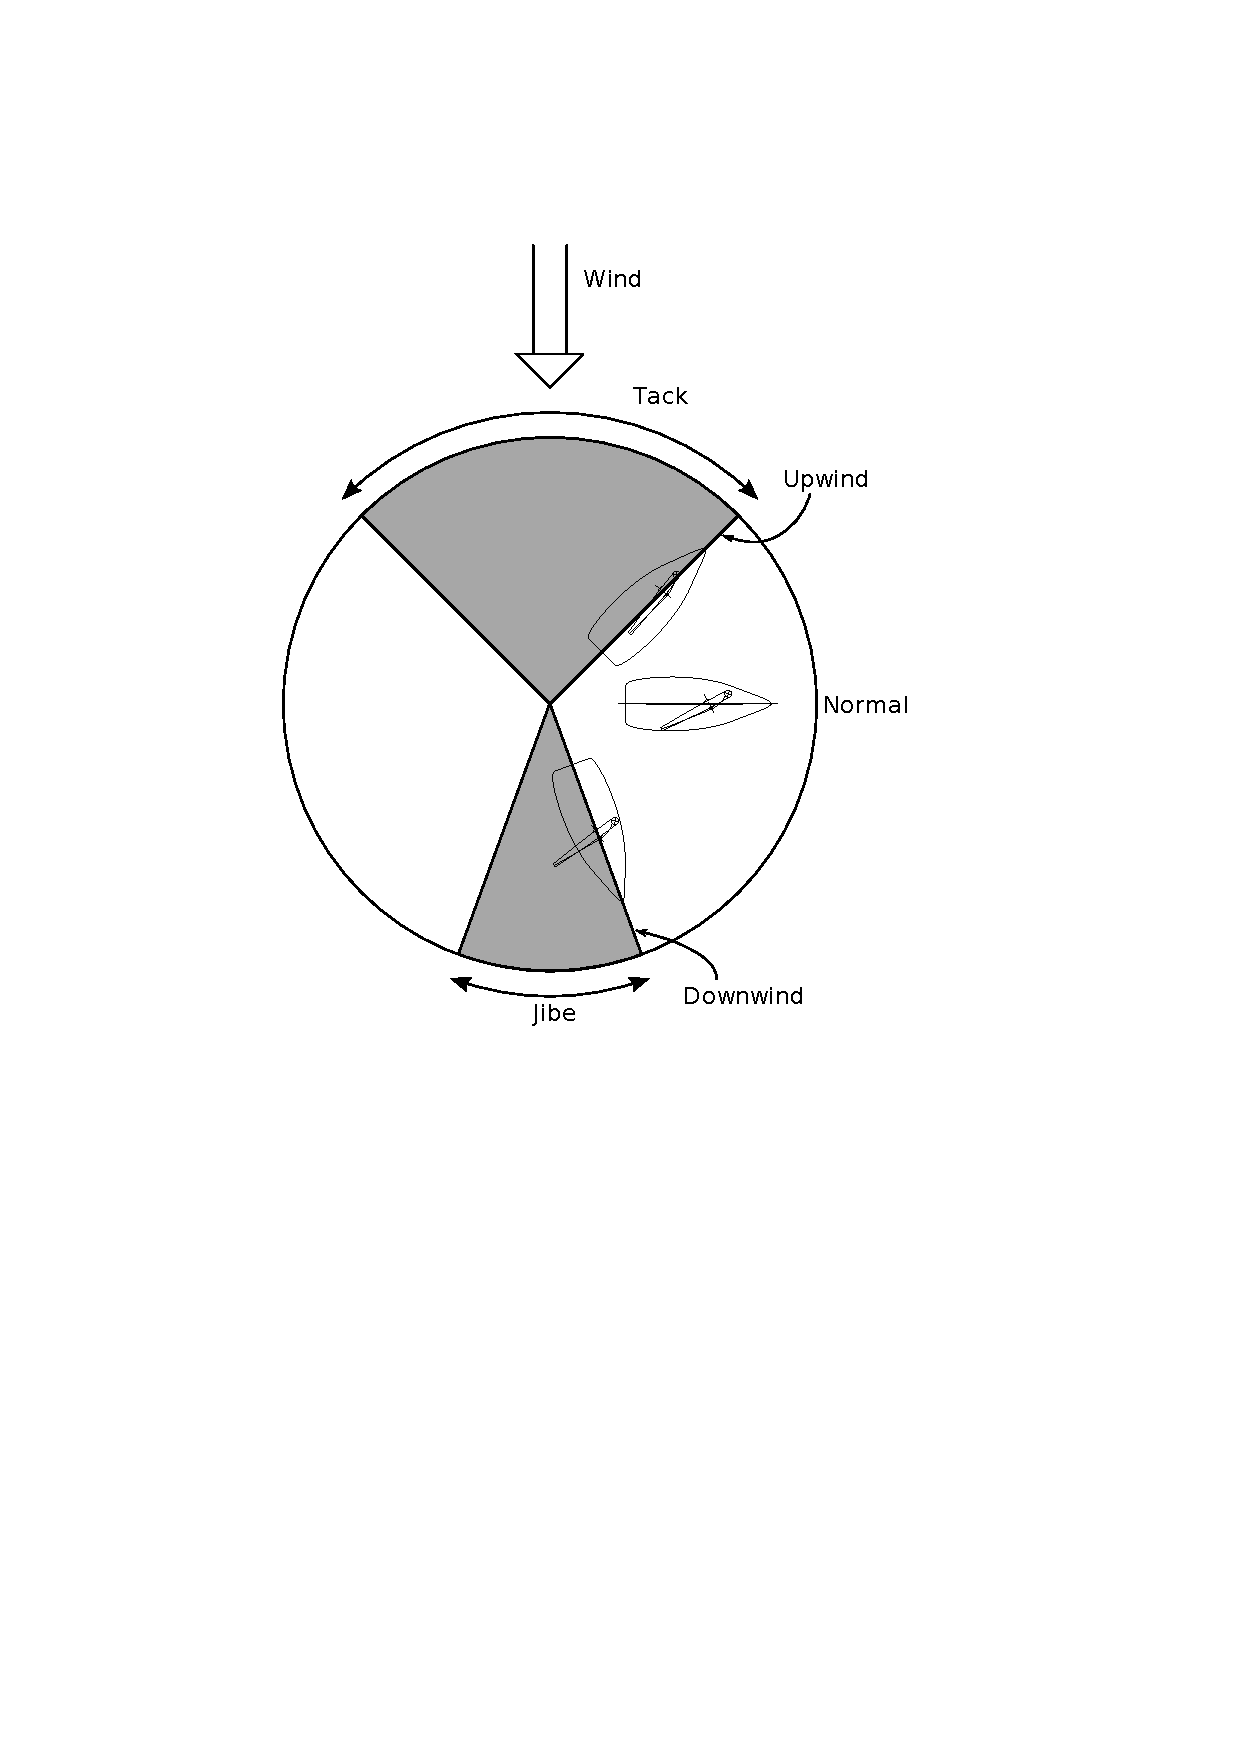
\includegraphics[trim = 45mm 120mm 55mm 45mm, clip, width=0.70\columnwidth]{pics/courses_to_wind.pdf}
\caption{Possible courses of a sailing yacht with respect to the wind and corresponding control system states. The range with wind directly from behind could be sailed in theory, but is not very efficient and rather unstable.}\label{fig:courses_to_wind}
\end{figure}
\subsubsection{Normal Sailing}
If the desired heading given by the path planner (section \ref{sec:navigator}) is
in the sailable (white) range, the system is in state \texttt{Normal Sailing}.
In this state the rudder controller follows the given desired heading, while
the sail controller permanently adjusts the sail to achieve the optimal angle
of attack on the sail. If the desired heading changes within the sailable
range, the rudder controller simply follows the new course while the sail
controller maintains a constant angle of attack.
\subsubsection{Upwind Sailing}
If the desired heading for whatever reason is set in the not sailable (gray)
range, it cannot be directly followed. The objective in this case is to make as
much velocity towards the wind as possible. In \texttt{Upwind Sailing} mode the
sail is set to the tightest position that is reasonably possible. While the
sail angle is kept at this constant position, the rudder controller now keeps a
constant heading angle to the true wind and thus takes advantage of all wind shifts.
Note that the behaviour is similar for downwind sailing.
%
\subsection{Test Results and Analysis} \label{sec:sailor_testing}
Several tests were undertaken to verify and optimise the control system. Before
any testing on the water was done, the state machine's transition conditions
had to be verified. This was done by putting the boat on a trailer on a
sufficiently windy day and turning it around its vertical axis while constantly
checking the current state. We encountered many problems that were caused by
the sign change between $-180^o$ and $+180^o$. Some time could have been saved,
if the whole control program, including the state machine, had been tested more
thoroughly in the simulation environment.

The controller was then tested for its ability to keep a desired heading and to
react to changes in desired heading. After some tuning of the PID parameters we
found that the parameters in table \ref{tab:pid_params} yield fast reactions
without too much overshoot.
%
\begin{table}[htb]
\caption{PID Parameters} \label{tab:pid_params}
\centering
\begin{tabular}{c|l}\hline
P & 0.3  \\ \hline
I & 0.005 \\ \hline
D & 30 \\ \hline
\end{tabular}
\end{table}
%
A step response in winds of about 20 knots is illustrated in figure
\ref{fig:step_response_wind20kn}. Note that 20 knots is already a strong wind
and that in lower wind speeds we experienced much less oscillation around the
reference value. Even this $\pm 10^o$ oscillation that is mostly caused by
waves can barely be seen on the boat. We then also applied disturbances to the
boat by deviating it from its course by hand. The reaction was the same as with
changes in desired heading.
%
\begin{figure}[thb]
\centering
% trim = left bottom right top
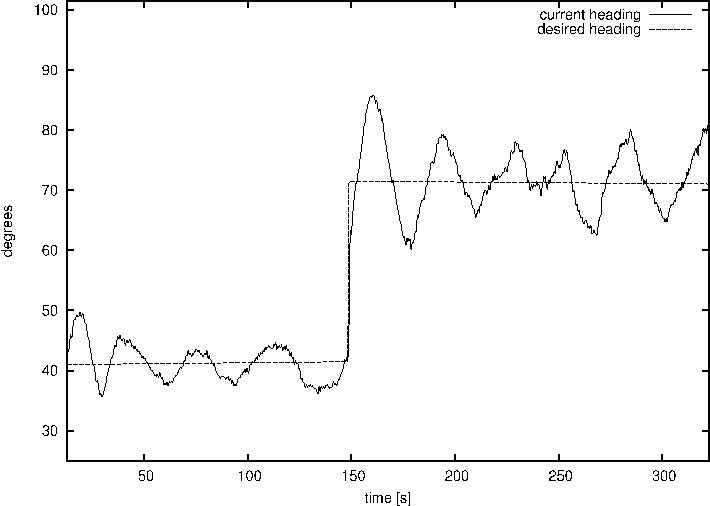
\includegraphics[trim = 0mm 0mm 0mm 0mm, clip, width=7cm]{pics/reference_step_usee4_2.pdf}
\caption{Step response in state \texttt{Normal Sailing}. Conditions were 20\,kn wind from 140°}\label{fig:step_response_wind20kn}
\end{figure}

Figure \ref{fig:3tacks_upwind_sailing} shows current heading, desired heading
and wind direction during three tacks. Between the tacks, the controller state
machine is in state \texttt{Upwind Sailing}. It can be very well seen, that the
boat keeps a constant angle to the wind and takes advantage of wind shifts as
expected.
\begin{figure}[thb]
\centering
% trim = left bottom right top
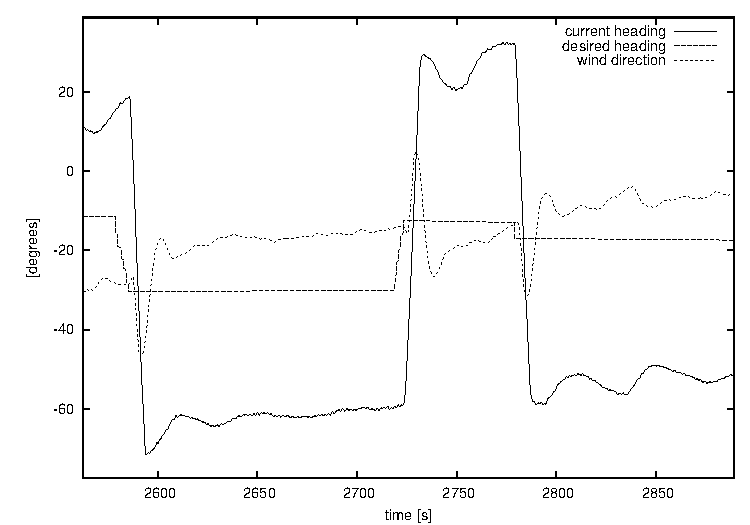
\includegraphics[trim = 0mm 0mm 0mm 0mm, clip, width=7cm]{pics/tacks_to_upwind_usee5_wind8kn_hdg.pdf}
\caption{3 tacks, with \texttt{Upwind Sailing} in between.}\label{fig:3tacks_upwind_sailing}
\end{figure}
A lot of time was invested into correct timing during tack and jibe. In the
beginning we had several problems that resulted in inappropriate sail tuning
during or right after manoeuvres. This sometimes even resulted in the boat
sailing backwards.

Figure \ref{fig:wyp_autonom_drift_comp} shows how the boat follows a trajectory
that was calculated by the path planner. The path planner's calculation was started
at the bottom left where the dashed line begins. After the calculation was
completed, the boat jibes and sets the new course. After a few seconds the
drift compensation starts to work and the boat's real course approaches the
desired trajectory.
%
\begin{figure}[thb]
\centering
% trim = left bottom right top
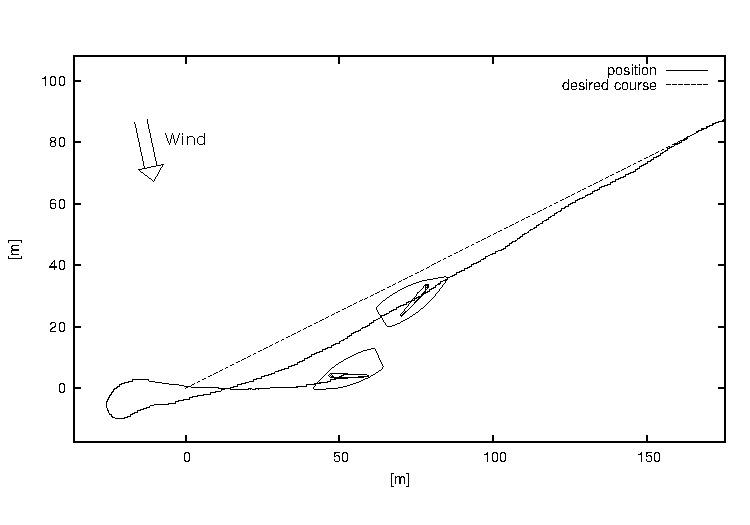
\includegraphics[trim = 0mm 0mm 0mm 0mm, clip, width=7cm]{pics/driftcompensation.pdf}
\caption{GPS plot of the controller following a desired trajectory calculated
by the path planner. It was recorded during a test on the Urnersee in about 15
knots wind.}\label{fig:wyp_autonom_drift_comp}
\end{figure}


\section{Path Planner} \label{sec:navigator}
\subsection{Principle of motion planning for a sailing boat} \label{sec:intro_principle}
Due to the nature of every sailing vessel, \textsc{Avalon}'s manoeuvrability is
limited in relation to wind direction. Additionally, due to the non-holonomic
properties of a sailing vessel, it is not possible to change the heading on the
spot immediately.  The trajectory tracker (see section \ref{sec:skipper}) has
to keep that in mind and operate in a way that allows a certain space to make
heading changes. For the implementation of a navigation algorithm, these
constraints imply that using accurate wind information for every calculation is
essential.
 
\subsection{Literature Research}
%
Path planning in the naval industry is not a new topic. For many years,
commercial ships have used weather forecasts to generate an optimal path with
respect to speed or bypassing bad weather situations. For sailing ships,
commercial solutions by companies like \textsc{B \& G} or \textsc{Northstar}
exist, but do not offer any possibility to be integrated into our embedded
system. Looking at different navigation and routing strategies, two
fundamentally different ideas emerge: Roland Stelzer \cite{stelzer2008}, who
has published his approach also for implementation in an autonomous sailing
boat, projects the speed vector on the target direction and tries to find a
sailable heading that maximises that projected speed vector. Although in small
scale it might find a good and fast path, this approach is not sufficient when
it comes to larger search areas with obstacles and additional inputs like
weather forecasts.

The other approach is to use grid based path planning algorithms that allow us
to generate optimal solutions considering the path from start to goal and
enable the integration of specific constraints (see section
\ref{sec:intro_principle}).

\textit{Breadth first method} and \textit{Depth first} are both based on a very
simple principle and serve as archetypes for many important algorithms
\cite{cormen2001}, but may result in very long running time. \textit{Dijkstra}
on the other hand is a directed search \cite{lavalle2006} and guarantees
optimal results. A* is a modified version of \textit{Dijkstra} that also
considers the heuristic distance estimate of the path from current position to
the destination \cite{hart1968}, which makes it more directed than
\textit{Dijkstra}. One of the problems of grid-based planning algorithms is
that the angles are artificially constrained. The Theta*-Algorithm
\cite{nash2007} deals with that handicap and produces more realistic looking
paths than A* or even smoothed A*. A further extension of A* is D*
\cite{stentz1995}, which incorporates dynamic changes (i. e. moving obstacles)
along the path and does not require to replan the whole path from current
position to destination anymore.

The proposed approach uses a simple A* algorithm which is modified to comply
with all the sailing constraints. It must also be noted that there is few
computation time constraints for a sailing boat crossing the Atlantic ocean.
Even if path planning requires a handful of minutes, this is still an
acceptable behaviour.
%
\subsection{Planning Strategy}
%
Considering the distance of about 4'200 nautical miles \textsc{Avalon} has to
sail on its journey across the Atlantic Ocean and its slow speed of
about 4 to 5 knots\footnote{1 knot is 1 nautical mile per hour}, it is essential to distinguish between a global and a local
planning. Global planning will be done by fixing way-points across the Atlantic
based on expert knowledge, weather and current analysis. The local planner will
then plan from current position to the next global way-point using wind data
from the on board sensor. The planning algorithm will be triggered and
controlled by a trajectory tracker (section \ref{sec:skipper}), which knows
exactly towards which way-point \textsc{Avalon} is sailing at the moment.
%
\subsection{Interfaces with the controller}
An important part of the software structure is the interface between the
navigation program and the control system (see section \ref{sec:sailor}). The main
reason why we decided to pass \textit{headings} instead of way-points from the
planner via the trajectory tracker to the controller, was that the planner calculates an optimal
path with respect to path duration for specific angles to the wind.
Drift that pushes the vessel off the trajectory will be handled by the controller,
a new calculation will only take place after the boat has a certain deviation
from the set trajectory (see section \ref{sec:skipper}).
\paragraph{Wind data}
The wind the local path planner uses is an average of the measurements over the last 90 seconds. The control system will then follow the received desired heading using a much more accurate wind direction that was averaged only over a period of 5 seconds (see section \ref{sec:sailor}). Figure \ref{fig:cleanwind} shows a comparison of the two different wind sets.
%
\begin{figure}
 \centering
 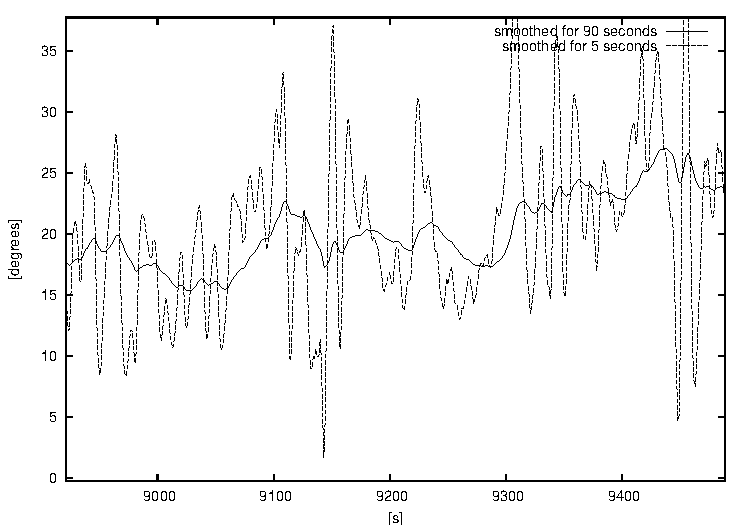
\includegraphics[width = 6.5 cm]{pics/paper_cleanwind.pdf}
 \caption{Differently filtered wind information}
 \label{fig:cleanwind}
\end{figure}

%
\subsection{Planning algorithm}
As explained earlier, \textit{Dijkstra}'s graph search is the basic algorithm
used to perform the path search. Starting at an initial grid-point, the algorithm expands over the whole field until the final grid-point has been reached. Every evaluated grid-point will be assigned a certain cost, a time estimate of how long it will take the boat to sail from the initial grid-point to the point that is currently being evaluated. The final optimal path is then determined by always following the neighbor with the lowest costs from the final to the initial grid-point. 

To be able to allocate costs for ship movements, i. e. moving from one grid-point to a neighbor, we work in 3 dimensions, with $x$ and $y$ for the geographic position
and $\theta$ for the heading of the boat at that position. To get sailable and
reasonable results, the following costs have been implemented additionally:
%
\begin{itemize}
\item Sailing-Time from start node
\item Estimated sailing time to the end node (heuristic)
\item Cost for heading changes
\item Cost for manoeuvres (tack and jibe)
\item Cost for offset from the straight connection between start and end node (tunnel cost).
\end{itemize}
%
\subsubsection{Grid compatible coordinate system}
To represent GPS points on a map, a coordinate transformation is necessary. Since we plan only for short distances ahead of us (local planning), we can use a very simplified transformation into meter coordinates 
\begin{equation}
\begin{array}{l}
 x = R_E \cdot \cos\left( \text{lat}\right) \cdot \dfrac{\pi}{180\, deg} \cdot \text{lon}\\
\\
 y = R_E \cdot\dfrac{\pi}{180\, deg}\cdot \text{lat}
\end{array}
\end{equation}
where $R_E$ is the earth radius, lon and lat the GPS coordinates in degrees. This transformation assumes a flat water surface \cite{stelzer2008}. In order to initialise the local map as small as possible, the algorithm places the origin as close as possible to either start or target coordinate. 
%
\subsubsection{Polar diagram}
In order to calculate the boat speed for a specific angle to the wind, a polar
diagram\footnote{In boating term, the polar diagram gives a boat velocity  as a
function of its  heading to the wind and the wind velocity} of \textsc{Avalon}
is needed.  Since creating a detailed diagram for our boat would require
constant wind and wave conditions over a long time, we created a polar diagram
based on existing diagrams for bigger vessels. Testing has shown that we get
reasonable results by restricting the sailable \textit{angle to the wind} to
the area between $45^o$ and $160^o$ (see figure \ref{fig:courses_to_wind}).
%
\subsubsection{Heading}
\hide{
% This is too much inmplementation dependent
We assume a 24 neighbour grid throughout this paper, which allows to have
sixteen different headings available for sailing. Another advantage of being
able to expand to the second but next neighbour-grid is the fact that it reduces
the number of way-points, since one grid node is skipped.
\subsubsection{Connectivity List}
In theory, every heading change is possible with a sailing boat. However, to
make the algorithm faster, we have constricted the biggest possible change of
heading to $90^o$. The areas that are not sailable due to the wind direction
are between $\pm45^o$ to wind direction for sailing upwind and $\pm160^o$ to
wind direction for sailing downwind (see figure \ref{fig:courses_to_wind}).
%
}
In order to limit the size of the 3D grid used in this paper, we use a
discretisation of the possible boat heading into 16 possible headings. In usual
2D grid-based path planning, transition from one cell to its 8 neighbours is
considered. This results in only 8 possible changes of orientation. By
considering a neighbourhood of 24 cells (8 cells around the starting cell, plus
16 cells one cell further), we can reach 16 different heading changes in one
transition. This leads to smoother paths and smaller number of way-points on the
final path.

We further reduce the computational complexity of the planner by considering
that the maximum change of heading in one transition is $90^o$. This
restriction is consistent with the experience of human skippers. 
%
\subsection{Cost Factors}
\subsubsection{General Costs}
The general aim of this algorithm is to find the shortest path for a sailing vessel to go from point $A$ to point $B$. The general cost we give for every movement is therefore \textit{sailing time to the next node}, calculated by equation \ref{eq:navi_timecost}. The speed solely depends on the angle to the wind and the wind speed. 
\begin{equation}
 \text{sailing time} = \frac{\text{distance to next node}}{\text{speed}} 
\label{eq:navi_timecost}
\end{equation}
\subsubsection{Heuristic Estimate}
The heuristic estimate is used to evaluate the remaining time to the goal.
According to \cite{lavalle2006}, the only constraint on the heuristic is that
it has to underestimate the real cost of the remaining path. For simplicity sake, the
heuristic returns the time it would take to sail to the goal at an exaggerated speed of 10 knots. More complicated options have been considered, but none of them provided well defined behaviour in all situations.

\subsubsection{Turning Cost}
To generate paths as smooth as possible, the algorithm places costs $C_{\text{new}}$ for heading changes, using a simple linear factor $f$ in equation
\begin{equation}
 C_{\text{new}} = f \cdot \vert \theta_{\text{curr}} - \theta_{\text{new}} \vert  
\label{eq:navi_turningcost}
\end{equation}
where $\theta_{\text{curr}}$ and $\theta_{\text{new}}$ are the respective headings. 
%
\subsubsection{Cost for Tack or Jibe}
By giving a certain cost for tack or jibe, we can indirectly control the number
of manoeuvres \textsc{Avalon} sails.  The principle is very simple, we check if
the sign of $(\theta_{\text{curr}} - \text{winddirection})$ and $(\theta_{\text{next}} -
\text{winddirection})$ is the same. If it is different, an additional cost will be
added to the total cost.
%
\subsubsection{Tunnel cost}
In order to favour paths that stay closer to the straight line path, we
allocate costs increasing with the distance from the direct connection of start
and target node. It has proved best to increase the cost only little for the
areas in the middle of the tunnel but increase it abruptly when closing in on
the borders. 
%
\subsubsection{Obstacle avoidance} 
To avoid islands and coastal regions, the algorithm gives extremely high costs
for passing prohibited terrain. To locate these areas, it parses information
from a map.\\
To avoid commercial ships on the Atlantic, \textsc{Avalon} can receive AIS
signals from most ships travelling over the Atlantic. Knowing ship speed,
direction and current position, our algorithm will place no-go areas around potential collision locations to make sure to bypass them.
%
% we had that already in chapter nav_strategy:
\hide{
\subsection{Trajectory tracker} \label{sec:skipper}
The trajectory tracker has mainly two important tasks:
\begin{itemize}
 \item Triggering the local planner
 \item Calculating a desired heading for the control system
\end{itemize}
\subsubsection{State machine}
To manage the different tasks, the trajectory tracker can switch between different states:
%
\paragraph{Standard Navigation}
If not approaching a target or buoy, this state generates headings for the control system, going from way-point to way-point.
If the wind changes more than $20$° or if the ship distances itself from the current trajectory for more than a predefined distance, a new calculation will be initiated. 
\paragraph{Goal Approach}
If approaching a target position, the trajectory tracker will always send a heading that is directing exactly towards that point.
\paragraph{Buoy Approach}
This is a state designed especially for short course racing. Due to regulations that always require a port-side surrounding of the regatta buoys, this state will - when approaching a buoy - always write a heading that will lead the boat around the buoy.
\paragraph{New Calculation}
In this state, the trajectory tracker manages and supervises the new calculation. After having checked that the new way-points have been stored, it switches back to \textit{Standard Navigation}
}
%
%
\subsection{Tests and Discussion}
\subsubsection{Testing environment}
Most tests and parameter optimization was done by visualising the generated
path on screen and discussing its quality. Figure \ref{fig:navi_path}
shows two calculated path examples, both having to pass an obstacle and dealing
with difficult wind direction like upwind and downwind. Analysis has shown that the addition of a tunnel cost is redundant since the heuristic estimate also favours paths that are close to the direct connection of {\em start} and {\em target} node. Although adding an artificial tunnel cost might not always result in optimal path solutions, we used the tunnel for safety reasons to make sure that the vessel never sails beyond predefined boundaries. 
\hide{
% In case of present obtacles, this is not always optimal.
\paragraph{Initial and final Heading}
Our initial motion was to set the current boat heading as $theta$ at the START
node. In case the TARGET was exactly in the opposite direction, the algorithm
then proposed a turn, which took about two to three way-points. Tests on the
water showed that this was not optimal at all and the manoeuvre cost us a lot of
time. We then set the START $theta$ directly towards the TARGET, which produced
much better results. One disadvantage is that the boat might sail away too far
from the starting point in case of long calculation time without receiving the
new heading. After calculation has finished, the trajectory tracker would then
notice the incoherence and trigger a new calculation. 
}

Another important and not yet solved problem is the final heading at the target
node that has to be known in order for \textit{Dijkstra} to start the search. At the
moment the algorithm chooses a final heading that is as close as possible to
the direct heading of a straight line from start to destination but always
differs at minimum $45^o$ from the wind direction. This usually produces good
results but it does not take obstacles into account which means that sometimes
an additional, unnecessary turn is produced. 

In practice, this issue will be solved by starting planning a new path before
completing the execution of the current one.


\begin{figure}[htb]
  \centering
  \subfloat[Upwind]{\label{fig:navi_upwind}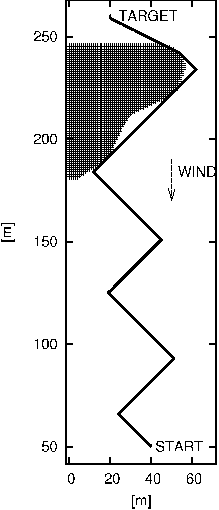
\includegraphics[width=2.7 cm]{pics/paper_kreuzen2.pdf}} 
  \hspace{1cm}
  \subfloat[Downwind]{\label{fig:navi_downwind}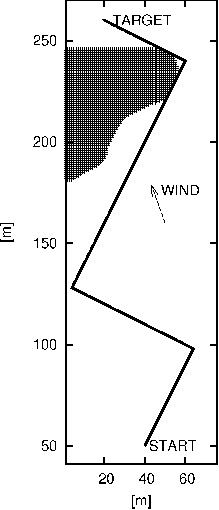
\includegraphics[width=2.7 cm]{pics/paper_downwind2.pdf}}
  \caption{Path examples for upwind and downwind sailing with obstacles}
  \label{fig:navi_path}
\end{figure}

\begin{figure}[htb]
\centering
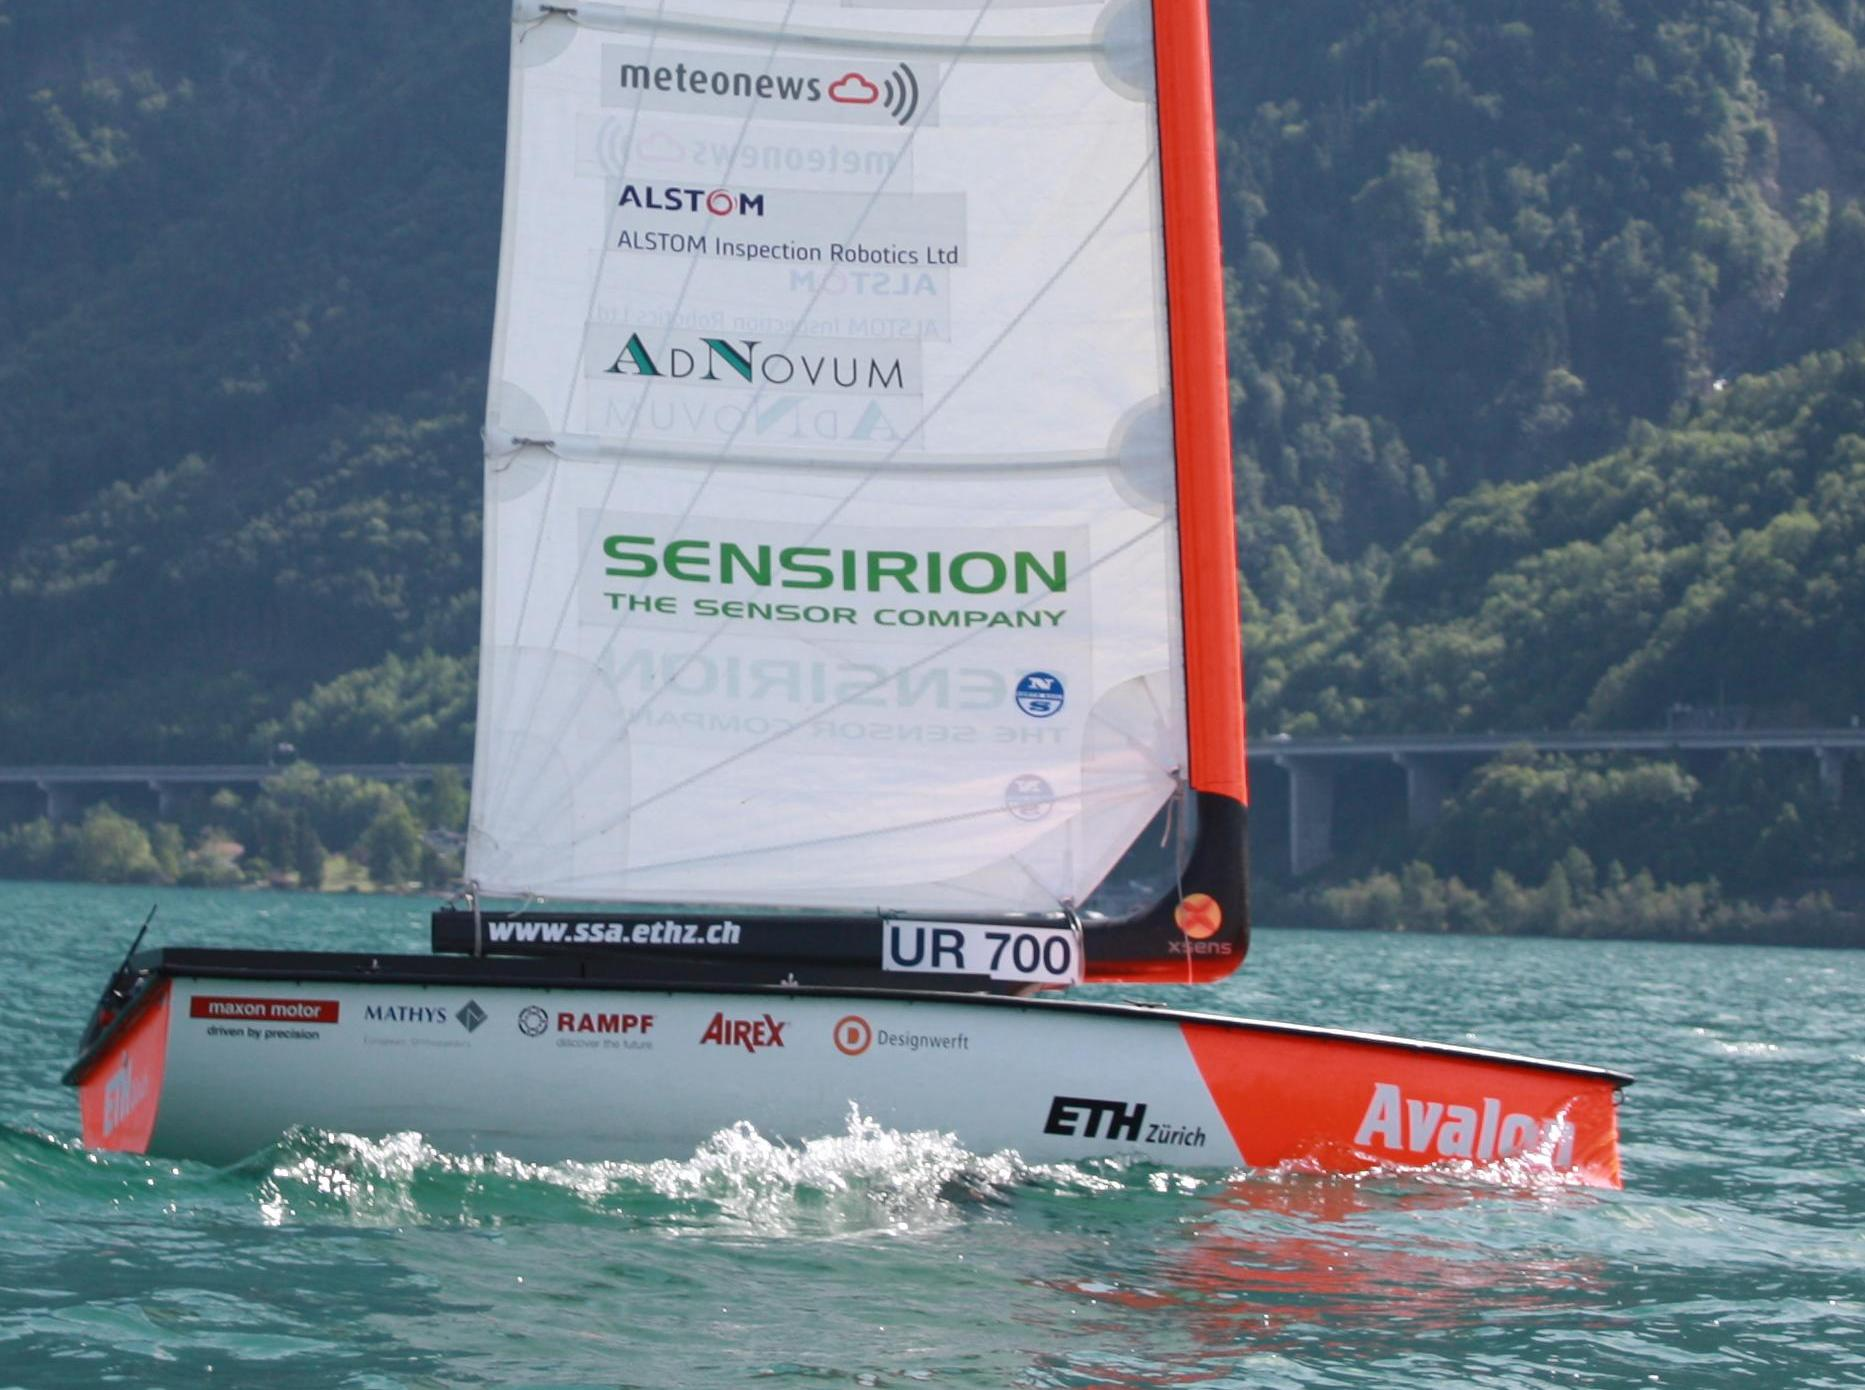
\includegraphics[width=0.75\columnwidth]{pics/IMG_0601_papercrop.jpeg}
\caption{Avalon during testing in high winds}
%\label{fig:avalon}
\end{figure}

\section{Conclusion and Outlook}
The proposed navigation and control software has been successfully implemented
in our autonomous sailboat \textsc{Avalon}. Several short-run tests both on
Swiss lakes and on the Atlantic Ocean have been carried out and have shown that the
described control and navigation system work. \textsc{Avalon} was exposed to
wind conditions ranging from almost 0 to 30 knots. The experimentally found
control parameters have proven to be well defined, keeping the vessel on course
even while sailing in rough sea states.

In very low wind speeds it was seen that the boat is able to sail much better
by itself than steered by us via remote control, because it is always aware of
the exact wind direction, even when human sailors hardly notice any wind at
all.

However, especially in reference to a possible crossing of the Atlantic Ocean,
several tests over a bigger period of time as well as longer distances have to
be performed in a next stage. 

By processing received AIS-signals, \textsc{Avalon} is able to identify other
ships in close proximity and therefore prevent collisions. However, small boats
that don't send position information cannot be recognized at this stage and
further research has to be done in identifying obstacles visually.   

Implementing a conventional and proved path planner like Dijkstra's for our
navigation system has proved well. Visually and analytically evaluated results
show that we achieve better solutions by taking the whole path into account
than by always optimising the heading at every current position. However, by
adding additional costs (like tunnel cost), optimal path solutions are not
always guaranteed.

Our goal for future work is to further optimise the software, especially
regarding energy consumption. For example a hysteresis could be added to the
sail tuner so that the sail does not constantly adapt to minor changes in wind
direction and speed. A further area of improvement could be in making use of
weather forecasts in the global navigation. For our boat this does not add much
value, because it is too slow to react to forecast weather changes.


% can use a bibliography generated by BibTeX as a .bbl file
% BibTeX documentation can be easily obtained at:
% http://www.ctan.org/tex-archive/biblio/bibtex/contrib/doc/
% The IEEEtran BibTeX style support page is at:
% http://www.michaelshell.org/tex/ieeetran/bibtex/
\bibliographystyle{IEEEtran}
\bibliography{IEEEabrv,ram_paper_ssa}

%

% Note that the a4paper option is mainly intended so that authors in
% countries using A4 can easily print to A4 and see how their papers will
% look in print - the typesetting of the document will not typically be
% affected with changes in paper size (but the bottom and side margins will).
% Use the testflow package mentioned above to verify correct handling of
% both paper sizes by the user's LaTeX system.
%
% Also note that the "draftcls" or "draftclsnofoot", not "draft", option
% should be used if it is desired that the figures are to be displayed in
% draft mode.
%
\documentclass[journal,final,letterpaper,twoside,twocolumn]{IEEEtran}
%\documentclass[journal,final,letterpaper,twoside,twocolumn]{IEEEtran}
% Add the compsoc option for Computer Society conferences.
%
% If IEEEtran.cls has not been installed into the LaTeX system files,
% manually specify the path to it like:
% \documentclass[conference]{../sty/IEEEtran}

\usepackage[utf8]{inputenc}        % Keybord settings


% Some very useful LaTeX packages include:
% (uncomment the ones you want to load)


% *** MISC UTILITY PACKAGES ***
%
%\usepackage{ifpdf}
% Heiko Oberdiek's ifpdf.sty is very useful if you need conditional
% compilation based on whether the output is pdf or dvi.
% usage:
% \ifpdf
%   % pdf code
% \else
%   % dvi code
% \fi
% The latest version of ifpdf.sty can be obtained from:
% http://www.ctan.org/tex-archive/macros/latex/contrib/oberdiek/
% Also, note that IEEEtran.cls V1.7 and later provides a builtin
% \ifCLASSINFOpdf conditional that works the same way.
% When switching from latex to pdflatex and vice-versa, the compiler may
% have to be run twice to clear warning/error messages.






% *** CITATION PACKAGES ***
%
\usepackage{cite}
\usepackage{textcomp}

% cite.sty was written by Donald Arseneau
% V1.6 and later of IEEEtran pre-defines the format of the cite.sty package
% \cite{} output to follow that of IEEE. Loading the cite package will
% result in citation numbers being automatically sorted and properly
% "compressed/ranged". e.g., [1], [9], [2], [7], [5], [6] without using
% cite.sty will become [1], [2], [5]--[7], [9] using cite.sty. cite.sty's
% \cite will automatically add leading space, if needed. Use cite.sty's
% noadjust option (cite.sty V3.8 and later) if you want to turn this off.
% cite.sty is already installed on most LaTeX systems. Be sure and use
% version 4.0 (2003-05-27) and later if using hyperref.sty. cite.sty does
% not currently provide for hyperlinked citations.
% The latest version can be obtained at:
% http://www.ctan.org/tex-archive/macros/latex/contrib/cite/
% The documentation is contained in the cite.sty file itself.






% *** GRAPHICS RELATED PACKAGES ***
%
\ifCLASSINFOpdf
  \usepackage[pdftex]{graphicx}
  % declare the path(s) where your graphic files are
  % \graphicspath{{../pdf/}{../jpeg/}}
  % and their extensions so you won't have to specify these with
  % every instance of \includegraphics
  % \DeclareGraphicsExtensions{.pdf,.jpeg,.png}
\else
  % or other class option (dvipsone, dvipdf, if not using dvips). graphicx
  % will default to the driver specified in the system graphics.cfg if no
  % driver is specified.
 \usepackage[dvips]{graphicx}
  % declare the path(s) where your graphic files are
  % \graphicspath{{../eps/}}
  % and their extensions so you won't have to specify these with
  % every instance of \includegraphics
  % \DeclareGraphicsExtensions{.eps}
\fi
% graphicx was written by David Carlisle and Sebastian Rahtz. It is
% required if you want graphics, photos, etc. graphicx.sty is already
% installed on most LaTeX systems. The latest version and documentation can
% be obtained at:
% http://www.ctan.org/tex-archive/macros/latex/required/graphics/
% Another good source of documentation is "Using Imported Graphics in
% LaTeX2e" by Keith Reckdahl which can be found as epslatex.ps or
% epslatex.pdf at: http://www.ctan.org/tex-archive/info/
%
% latex, and pdflatex in dvi mode, support graphics in encapsulated
% postscript (.eps) format. pdflatex in pdf mode supports graphics
% in .pdf, .jpeg, .png and .mps (metapost) formats. Users should ensure
% that all non-photo figures use a vector format (.eps, .pdf, .mps) and
% not a bitmapped formats (.jpeg, .png). IEEE frowns on bitmapped formats
% which can result in "jaggedy"/blurry rendering of lines and letters as
% well as large increases in file sizes.
%
% You can find documentation about the pdfTeX application at:
% http://www.tug.org/applications/pdftex





% *** MATH PACKAGES ***
%
\usepackage[cmex10]{amsmath}
% A popular package from the American Mathematical Society that provides
% many useful and powerful commands for dealing with mathematics. If using
% it, be sure to load this package with the cmex10 option to ensure that
% only type 1 fonts will utilized at all point sizes. Without this option,
% it is possible that some math symbols, particularly those within
% footnotes, will be rendered in bitmap form which will result in a
% document that can not be IEEE Xplore compliant!
%
% Also, note that the amsmath package sets \interdisplaylinepenalty to 10000
% thus preventing page breaks from occurring within multiline equations. Use:
%\interdisplaylinepenalty=2500
% after loading amsmath to restore such page breaks as IEEEtran.cls normally
% does. amsmath.sty is already installed on most LaTeX systems. The latest
% version and documentation can be obtained at:
% http://www.ctan.org/tex-archive/macros/latex/required/amslatex/math/





% *** SPECIALIZED LIST PACKAGES ***
%
%\usepackage{algorithmic}
% algorithmic.sty was written by Peter Williams and Rogerio Brito.
% This package provides an algorithmic environment fo describing algorithms.
% You can use the algorithmic environment in-text or within a figure
% environment to provide for a floating algorithm. Do NOT use the algorithm
% floating environment provided by algorithm.sty (by the same authors) or
% algorithm2e.sty (by Christophe Fiorio) as IEEE does not use dedicated
% algorithm float types and packages that provide these will not provide
% correct IEEE style captions. The latest version and documentation of
% algorithmic.sty can be obtained at:
% http://www.ctan.org/tex-archive/macros/latex/contrib/algorithms/
% There is also a support site at:
% http://algorithms.berlios.de/index.html
% Also of interest may be the (relatively newer and more customizable)
% algorithmicx.sty package by Szasz Janos:
% http://www.ctan.org/tex-archive/macros/latex/contrib/algorithmicx/




% *** ALIGNMENT PACKAGES ***
%
%\usepackage{array}
% Frank Mittelbach's and David Carlisle's array.sty patches and improves
% the standard LaTeX2e array and tabular environments to provide better
% appearance and additional user controls. As the default LaTeX2e table
% generation code is lacking to the point of almost being broken with
% respect to the quality of the end results, all users are strongly
% advised to use an enhanced (at the very least that provided by array.sty)
% set of table tools. array.sty is already installed on most systems. The
% latest version and documentation can be obtained at:
% http://www.ctan.org/tex-archive/macros/latex/required/tools/


%\usepackage{mdwmath}
%\usepackage{mdwtab}
% Also highly recommended is Mark Wooding's extremely powerful MDW tools,
% especially mdwmath.sty and mdwtab.sty which are used to format equations
% and tables, respectively. The MDWtools set is already installed on most
% LaTeX systems. The lastest version and documentation is available at:
% http://www.ctan.org/tex-archive/macros/latex/contrib/mdwtools/


% IEEEtran contains the IEEEeqnarray family of commands that can be used to
% generate multiline equations as well as matrices, tables, etc., of high
% quality.


%\usepackage{eqparbox}
% Also of notable interest is Scott Pakin's eqparbox package for creating
% (automatically sized) equal width boxes - aka "natural width parboxes".
% Available at:
% http://www.ctan.org/tex-archive/macros/latex/contrib/eqparbox/





% *** SUBFIGURE PACKAGES ***
%\usepackage[tight,footnotesize]{subfig}
% subfigure.sty was written by Steven Douglas Cochran. This package makes it
% easy to put subfigures in your figures. e.g., "Figure 1a and 1b". For IEEE
% work, it is a good idea to load it with the tight package option to reduce
% the amount of white space around the subfigures. subfigure.sty is already
% installed on most LaTeX systems. The latest version and documentation can
% be obtained at:
% http://www.ctan.org/tex-archive/obsolete/macros/latex/contrib/subfigure/
% subfigure.sty has been superceeded by subfig.sty.



\usepackage[caption=false]{caption}
\usepackage[font=footnotesize]{subfig}
% subfig.sty, also written by Steven Douglas Cochran, is the modern
% replacement for subfigure.sty. However, subfig.sty requires and
% automatically loads Axel Sommerfeldt's caption.sty which will override
% IEEEtran.cls handling of captions and this will result in nonIEEE style
% figure/table captions. To prevent this problem, be sure and preload
% caption.sty with its "caption=false" package option. This is will preserve
% IEEEtran.cls handing of captions. Version 1.3 (2005/06/28) and later
% (recommended due to many improvements over 1.2) of subfig.sty supports
% the caption=false option directly:
%\usepackage[caption=false,font=footnotesize]{subfig}
%
% The latest version and documentation can be obtained at:
% http://www.ctan.org/tex-archive/macros/latex/contrib/subfig/
% The latest version and documentation of caption.sty can be obtained at:
% http://www.ctan.org/tex-archive/macros/latex/contrib/caption/




% *** FLOAT PACKAGES ***
%
%\usepackage{fixltx2e}
% fixltx2e, the successor to the earlier fix2col.sty, was written by
% Frank Mittelbach and David Carlisle. This package corrects a few problems
% in the LaTeX2e kernel, the most notable of which is that in current
% LaTeX2e releases, the ordering of single and double column floats is not
% guaranteed to be preserved. Thus, an unpatched LaTeX2e can allow a
% single column figure to be placed prior to an earlier double column
% figure. The latest version and documentation can be found at:
% http://www.ctan.org/tex-archive/macros/latex/base/



%\usepackage{stfloats}
% stfloats.sty was written by Sigitas Tolusis. This package gives LaTeX2e
% the ability to do double column floats at the bottom of the page as well
% as the top. (e.g., "\begin{figure*}[!b]" is not normally possible in
% LaTeX2e). It also provides a command:
%\fnbelowfloat
% to enable the placement of footnotes below bottom floats (the standard
% LaTeX2e kernel puts them above bottom floats). This is an invasive package
% which rewrites many portions of the LaTeX2e float routines. It may not work
% with other packages that modify the LaTeX2e float routines. The latest
% version and documentation can be obtained at:
% http://www.ctan.org/tex-archive/macros/latex/contrib/sttools/
% Documentation is contained in the stfloats.sty comments as well as in the
% presfull.pdf file. Do not use the stfloats baselinefloat ability as IEEE
% does not allow \baselineskip to stretch. Authors submitting work to the
% IEEE should note that IEEE rarely uses double column equations and
% that authors should try to avoid such use. Do not be tempted to use the
% cuted.sty or midfloat.sty packages (also by Sigitas Tolusis) as IEEE does
% not format its papers in such ways.




% *** PDF, URL AND HYPERLINK PACKAGES ***
%
%\usepackage{url}
% url.sty was written by Donald Arseneau. It provides better support for
% handling and breaking URLs. url.sty is already installed on most LaTeX
% systems. The latest version can be obtained at:
% http://www.ctan.org/tex-archive/macros/latex/contrib/misc/
% Read the url.sty source comments for usage information. Basically,
% \url{my_url_here}.





% *** Do not adjust lengths that control margins, column widths, etc. ***
% *** Do not use packages that alter fonts (such as pslatex).         ***
% There should be no need to do such things with IEEEtran.cls V1.6 and later.
% (Unless specifically asked to do so by the journal or conference you plan
% to submit to, of course. )


% correct bad hyphenation here
\hyphenation{op-tical net-works semi-conduc-tor middle-ware}

\newcommand{\hide}[1]{}
\begin{document}
%
% paper title
% can use linebreaks \\ within to get better formatting as desired
\title{Navigation Strategy and Trajectory Following Controller for an Autonomous Sailing Vessel}



% author names and affiliations
% use a multiple column layout for up to three different
% affiliations



%\author{

%\IEEEauthorblockN{Sebastian Boehl\IEEEauthorrefmark{1}}

%\and

%\IEEEauthorblockN{Lian P. Giger}
%\IEEEauthorblockA{ETH\\Federal Institute of Technology\\
%Zurich, Switzerland\\
%Email: ligiger@student.ethz.ch}

%\and

%\IEEEauthorblockN{Stefan Wismer} \IEEEauthorblockA{ETH Zurich}}

% conference papers do not typically use \thanks and this command
% is locked out in conference mode. If really needed, such as for
% the acknowledgment of grants, issue a \IEEEoverridecommandlockouts
% after \documentclass

% for over three affiliations, or if they all won't fit within the width
% of the page, use this alternative format:
%
\author{\IEEEauthorblockN{Hendrik Erckens ({\small corresponding author}), Gion-Andri Büsser,\\Dr. C\'{e}dric Pradalier, Prof Dr. Roland Y. Siegwart\\ \IEEEauthorblockA{Autonomous Systems Lab, Swiss Federal
Institute of Technology (ETH) Zurich\\Leonhardstrasse 25, 8092 Zurich, Switzerland \\
E-mail: herckens@student.ethz.ch}}}

% use for special paper notices
%\IEEEspecialpapernotice{(Invited Paper)}

% make the title area
\maketitle
\begin{abstract}
%\boldmath
This paper describes the design and implementation of a navigation and control
system for the autonomous sailing
vessel {\sc Avalon}. This boat, designed for participating in the {\sc
Microtransat}, is engineered to autonomously cross the Atlantic Ocean. We
present here a specially robust mechanical design and the navigation software
that will plan an optimal navigation course and efficiently control the boat on
this course. The path planner uses an A* algorithm to generate the fastest path
to a given destination. It is able to avoid both static and dynamic obstacles.
By using a given polar diagram and measured wind data, it takes into account
manoeuvrability constraints of a sailboat. The control system takes care of
rudder and sail in order to follow a given heading while optimising speed.
Additionally, the system is capable of automatically conducting manoeuvres such
as tack and jibe. 
At the time of this writing, {\sc Avalon} and its software systems have been
successfully tested more than two weeks in short deployments lasting several
hours with winds ranging from 0 up to 30 knots. 
\end{abstract}
% IEEEtran.cls defaults to using nonbold math in the Abstract.
% This preserves the distinction between vectors and scalars. However,
% if the conference you are submitting to favors bold math in the abstract,
% then you can use LaTeX's standard command \boldmath at the very start
% of the abstract to achieve this. Many IEEE journals/conferences frown on
% math in the abstract anyway.
%
% no keywords
%
% For peer review papers, you can put extra information on the cover
% page as needed:
% \ifCLASSOPTIONpeerreview
% \begin{center} \bfseries EDICS Category: 3-BBND \end{center}
% \fi
%
% For peerreview papers, this IEEEtran command inserts a page break and
% creates the second title. It will be ignored for other modes.
% \IEEEpeerreviewmaketitle
%
\section{Introduction}
%\subsection{General Objectives for building an autonomous sailboat}
This paper introduces the autonomous sailboat \textsc{Avalon} as seen in figure
\ref{fig:avalon}. The general objective for building an autonomous sailing
vessel is to further research and development in the area of unmanned,
autonomous robotic vehicles that are exposed to heavy environmental conditions
such as the Atlantic Ocean. It has been established that there is a demand for
autonomous sailboats to be used for ocean sampling and surveillance
\cite{cruz:ase} but also for the implementation of this type of software in
manned sailing vessels. Either by passively proposing optimal sailing routes or
by actively supporting the sailor in dangerous situations by piloting the sail
or rudders, an integrated autonomous sailing system could back up and
facilitate a lot of situations. For example, if a single hand sailor falls over
board, the system could detect this incident and automatically execute a Man
Over Board manoeuvre.

\subsection{Our Goals and Objectives for this Work}
Our boat \textsc{Avalon} was designed to compete in the \textsc{Microtransat}
Challenge and thus has to withstand the harsh conditions on the Atlantic Ocean.

The goal of this paper is to present a software that is
capable of calculating the optimal path to reach a given destination as quickly
as possible, and the design of a controller able to safely and efficiently
guide the sailboat along the calculated path, taking into account the current
environmental conditions, such as wind speed.
\hide{Furthermore, it should be able to respond to a possible shortness of
energy by adjusting the control parameters or changing the mode of sailing.}


\subsection{Review of Existing Autonomous Sailing Boats}
An autonomous sailboat has to be capable of sailing without human intervention.
That means, that all tasks that are normally carried out by the sailor on a
conventional sailboat have to be done autonomously. That involves navigation
as well as working the rudder and sail in order to steer the defined course.
Other autonomous sailboats have been developed mostly by \textsc{Microtransat}
participants \cite{briere2008iar}, \cite{stelzer2008}, \cite{alves:fas},
\cite{sauze2008dcs}, but also commercially usable products \cite{harborwing}
have been built. In contrast to most of the existing work, we use a path
planner to avoid obstacles. Additionally, our controller switches between many
different modes of sailing, in order to make better use of wind shifts.

\section{A Boat Designed for Survival}
To provide an insight into the platform that was used to implement the proposed
software, this section summarises some details about the main components of
{\sc Avalon}. The mechanical system was more comprehensively described in
\cite{giger2009}. Table \ref{tab:avalon_data} shows the major technical details
of {\sc Avalon}.
\begin{figure}[b!]
\centering
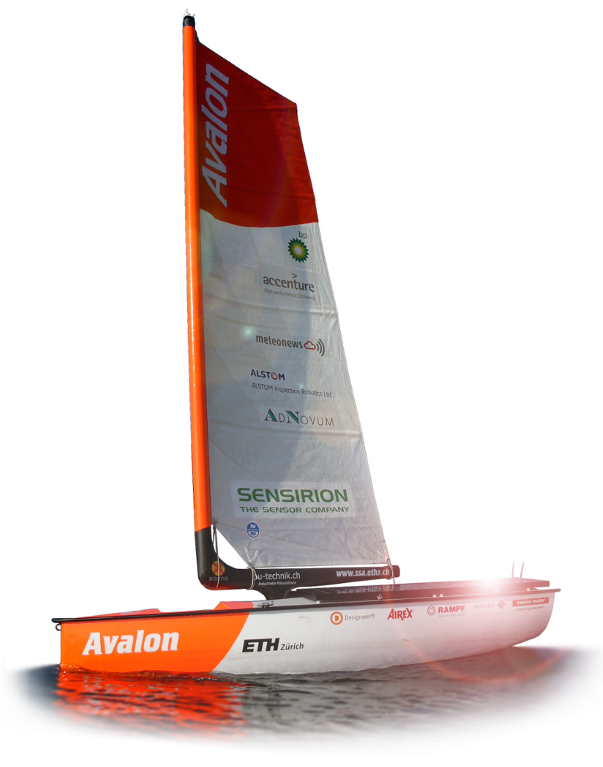
\includegraphics[height=0.8\columnwidth]{pics/avalon.png}
\caption{Avalon ready to sail on the lake of Z\"urich}
\label{fig:avalon}
\end{figure}

\subsection{Rig}
The rigging system is one of the most important parts of the whole
assembly. A defect in its structure will inevitably cause the whole project to
fail. The following aspects were considered for the design:
\begin{itemize}
\item High loads and forces on the mechanical structures due to
strong winds and heavy weather conditions.
\item Highest demands on reliability. There is no chance to
repair anything throughout the journey.
\item Preferably efficient force transmission from the actuator to the sail in order to save as much energy as
possible
\end{itemize}

During the design phase it turned out that a balanced rig prevails over a
conventional rig.
\hide{
The balanced rig is much more efficient regarding energy
consumption than any other conventional rig. The force needed to position the
sail is reduced by over 50\% due to the balanced distribution of
the sail load. Furthermore, }\textsc{Avalon}'s rig does not use any ropes
that could generate knots and jams. It is pivoted on a central
bearing without shrouds and stays. The result is a simple and reliable construction.
%
\subsection{Hull}
\hide{The hull design is based on form parameters, e.g. length, draft and
beam. Parameters were used as input data for B-spline curves and
surfaces. Instead of modifying those curves and surfaces, we used
constrained optimisation algorithms to generate the geometry. The algorithm
minimises a target function, which is defined so that a certain combination of
parameters results in a desired hull shape.}

The hull was designed using the CAE software \textsc{FRIENDSHIP-Framework} and
was laminated inside a female mold using glass fibre
sandwich. Epoxide resin was sucked into dry glass fibre material by
vacuum in a so called \textit{Infusion Process}. Compared to
conventional laminating, this method is much cleaner and more
convenient.

%---------------------------------------------------------
%basicdata: AVALON
%---------------------------------------------------------
\begin{table}[htb]

    \begin{center}
     \caption{Technical Data of \textsc{Avalon}}
	\label{tab:avalon_data}
%        \begin{tabular}[h!]{p{0.15\textwidth}| p{0.2\textwidth}| p{0.05\textwidth}}
        \begin{tabular}[htb]{l|l|l}
            \hline
            \emph{Variable}    &   \emph{Description} &   \emph{Value}\\ \hline\hline
            $L_{OA}$    &   Length over all	& $3.95\,m$\\
            $B_{max}$   &   Maximal beam	& $0.7\,m$\\
            $T$         &   Draft without keel  & $0.25\,m$\\
            $D_{max}$	&   Draft over all	& $2\,m$\\
            $H_{rigg}$	&   Height of the rigg  & $5.7\,m$\\
            $A_{sail}$	&   Total sail area     & $8.4\,m^2$\\
            $\nabla$    &   Submerged volume    & $0.44\,m^3$\\
            \hline
        \end{tabular}
    \end{center}
\end{table}


\begin{figure}[htb]
\centering
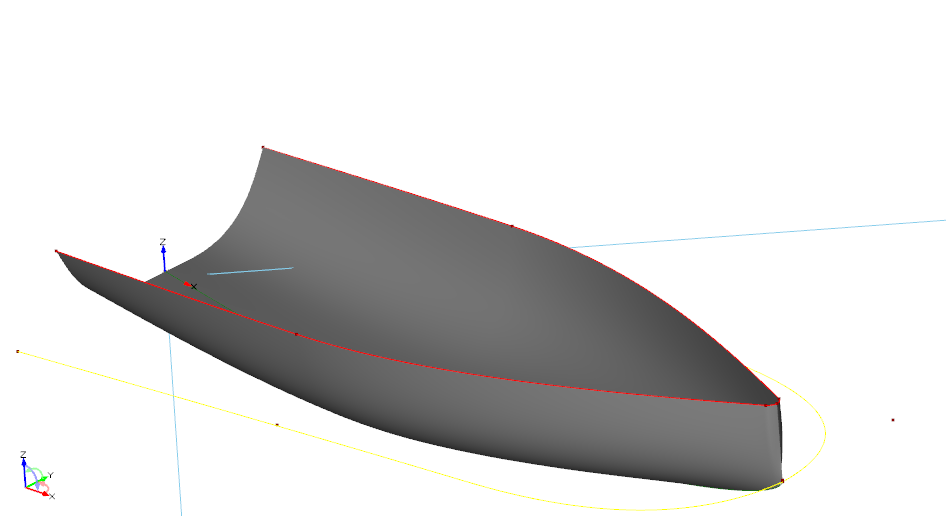
\includegraphics[width=0.37\textwidth]{pics/hull.png}
\caption{Hull} \label{fig:hull}
\end{figure}

%
\subsection{Keel and Rudder}
\subsubsection{Keel}
In order to achieve a sufficient righting moment and stability
during heavy weather situations, {\sc Avalon}'s keel with a draft of
two meters consists of a slim fin with a 160\,kg ballast bulb.

The fin and parts of the bulb were made of high-modulus carbon fibre
in precisely milled polyurethane female molds. After hardening and
tempering, the bulb was filled with lead and the two halves were
glued together.

\begin{figure}[htb]
\centering
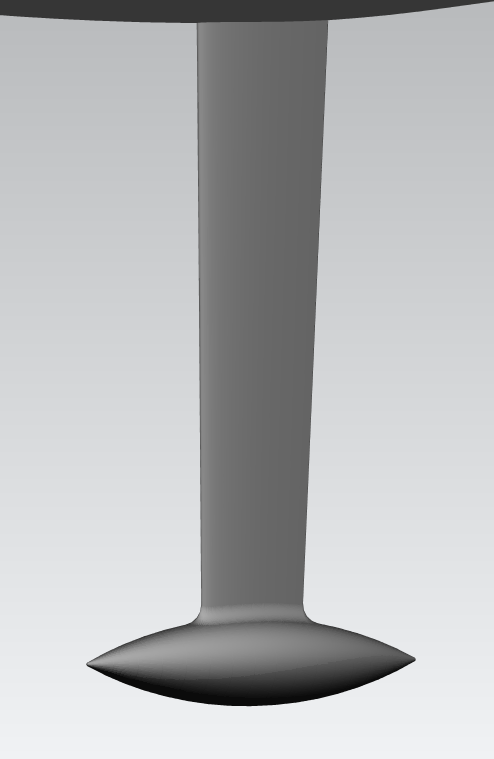
\includegraphics[width=2.7cm]{pics/keel.png}\hfill
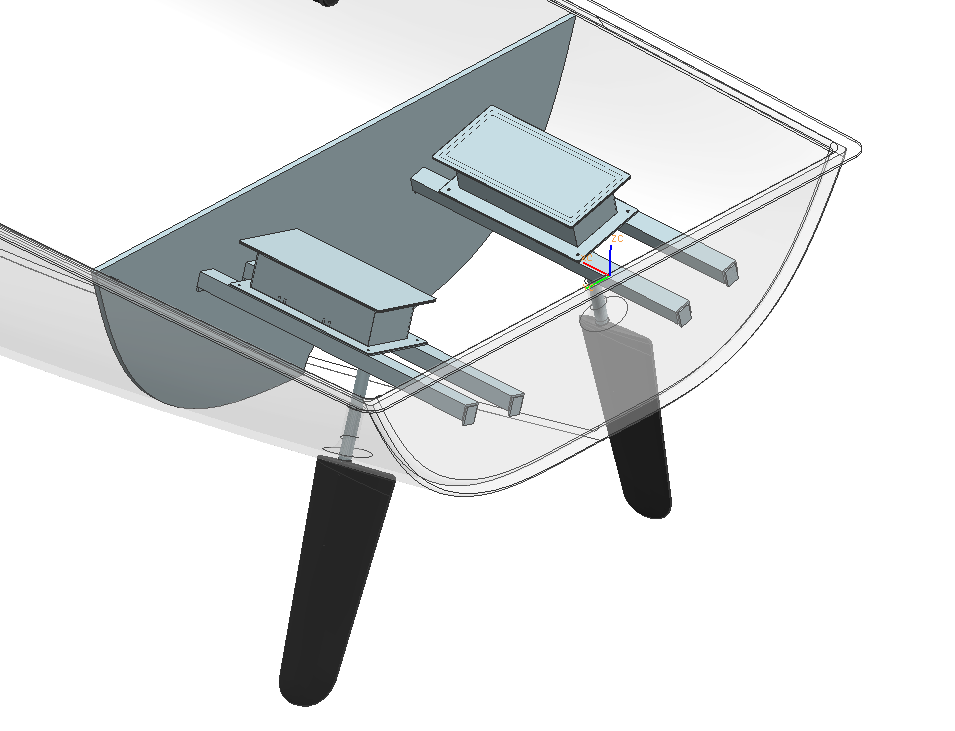
\includegraphics[width=4.5cm]{pics/rudder.png}
% \caption{Twin rudder system} \label{fig:cadrudder}
\caption{Keel with fin and ballast bulb (left), Twin rudder system (right)} \label{fig:cadkeel}
\end{figure}

\subsubsection{Rudder}
A twin-rudder system was selected for {\sc Avalon} to make sure to
have sufficient steering effect in every sailing situation. Angular
mounted twin-rudders provide better control at high
heeling angles compared to single rudders.

Assembled inside the hull, the rudder actuators are well sealed and
protected against water and humidity.

% \begin{figure}[htb]
% \centering
% 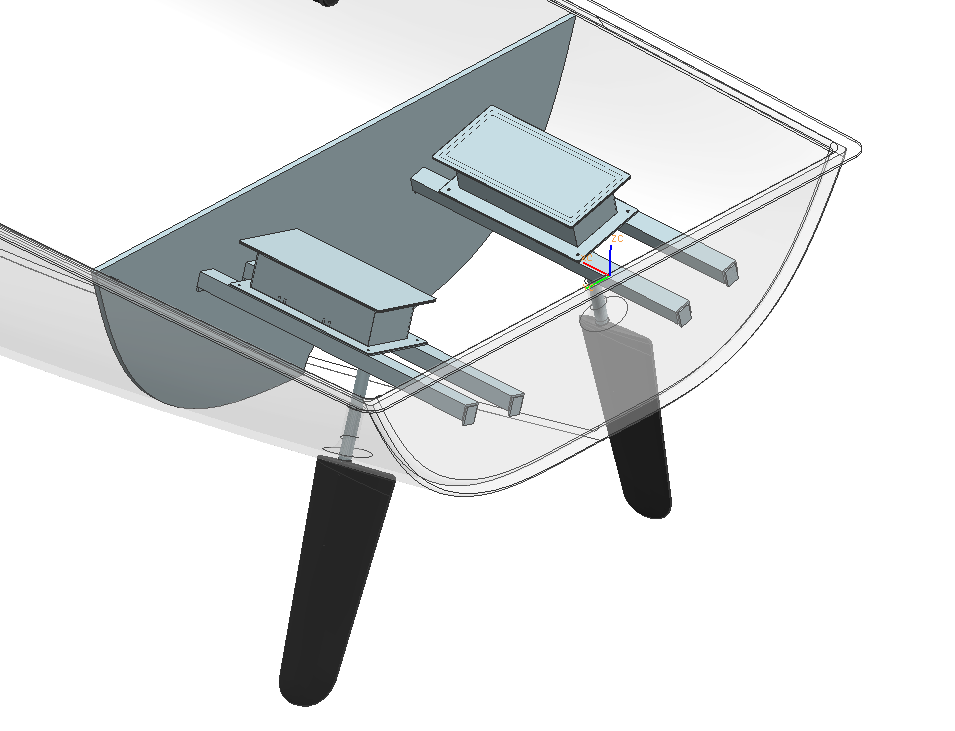
\includegraphics[width=4cm]{pics/rudder.png}
% \caption{Twin rudder system} \label{fig:cadrudder}
% \end{figure}
%
\subsection{Power Supply}
The main power supply is realised through two square meters of solar panels providing
a total of 360\,Wp. The collected energy is stored in four lithium-manganese
batteries. Each battery consists of 70 single cells and has a capacity of
600\,Wh at a nominal voltage of 25.2\,volts. Lithium-manganese batteries were
chosen mainly because of their weight but also because they are fairly safe to
use.

For back-up power, the boat has a direct-methanol fuel cell on
board. This fuel cell is automatically activated when the voltage
drops under a certain value, the \emph{switch on} voltage. It then
charges the batteries until the \emph{switch off} voltage is
reached. In theory, the solar cells provide enough power for the
boat's systems. The fuel cell only serves in case of enduring bad
weather  or other unforeseeable circumstances.



\section{Navigation Stategy}
This chapter will give a general overview of the software developed for
\textsc{Avalon} and discuss the interaction between control system and path
planner. Sections \ref{sec:sailor} and \ref{sec:navigator} will then go further
into details of the actual controller and path planner respectively.

The core hardware part and the brain of the system on the sailing vessel is the
main computer MPC21 from {\sc DigitalLogic}, a 500\,MHz device with 1024\,MB
RAM and a compact flash hard-drive. The device has an average power consumption
of about 8\,watts, the protection of a metal housing and a total weight of less
than 1\,kg.
% \begin{figure}[htb]
% \centering
% 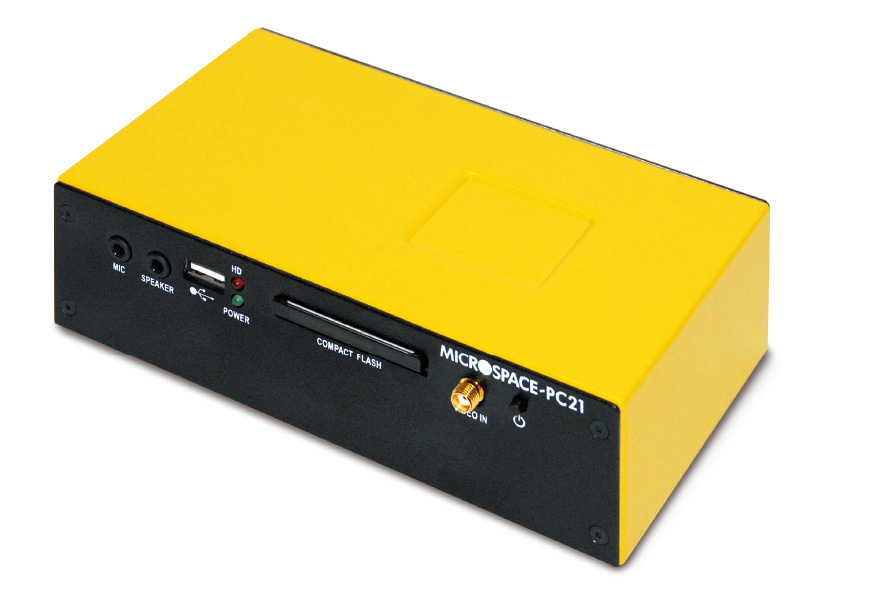
\includegraphics[height=4.0cm]{pics/RE_MPC21.png}\label{fig:mainpc}
% \caption{Main PC and brain of {\sc Avalon}\cite{digitallogic}}
% \end{figure}
%
The base of the entire software structure is the middleware DDX\cite{ddxpaper}
that runs on a Linux Operating System. This software manages a shared memory
called the Store and thus provides a means of communication between individual
programs that all run in parallel (see figure \ref{fig:ddx}). 

Sensor drivers will collect data from the specific sensors (see section
\ref{sec:sensors}) and store it in the DDX Store, from where it can be accessed
by the control and path planning programs.
% 
% A distinct advantage of DDX is the modular software structure. If ever a
% program crashes, it can be restarted without interrupting the other processes.
The different subprograms used on \textsc{Avalon} are depicted in figure
\ref{fig:ddx}.

\begin{figure}[htb]
\centering
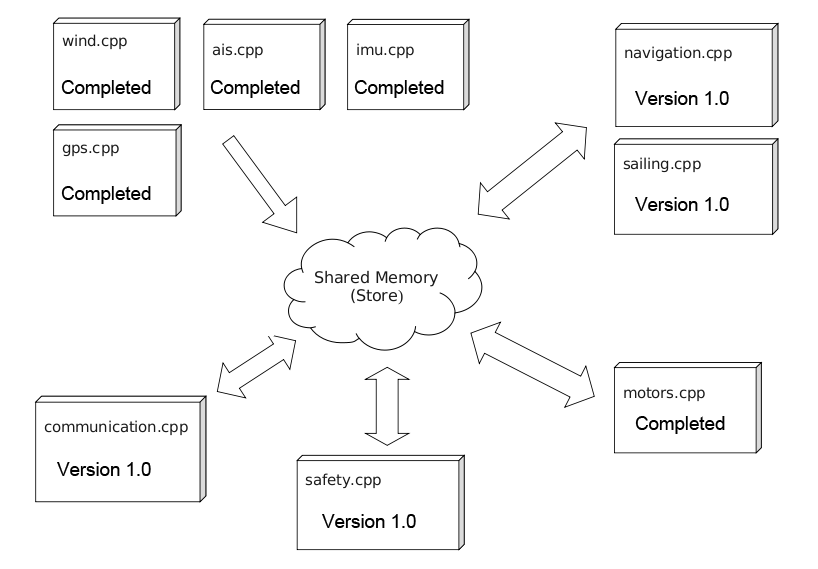
\includegraphics[height=5.5cm]{pics/RE_ddxplain.png}
\caption{Software organisation} \label{fig:ddx}
\end{figure}

%
%
\subsection{Sensors} \label{sec:sensors}
All desired information such as position, heading or speed are measured by
several sensors located all over the boat. To get a fully controllable system,
data is collected from the following sensors:
%
%\begin{description}[\IEEEsetlabelwidth{Wind}\IEEEusemathlabelsep]
%\item[\textbf{GPS}] 
\subsubsection{GPS \& IMU} 
%Provides position, heading and speed. The sensor's antenna is mounted on top of the mast. The electronic unit is located in the hull.
%\item[\textbf{IMU}]
The localization of the boat is performed by an \textit{Inertial Measurement
Unit} (by \textsc{X-Sens}) that is combined with a GPS receiver. Using the
accelerations in all 6 degrees of freedom and a high update rate of 120 Hz,
occasional deviations of the GPS-data will automatically be smoothed out. The
system therefore produces highly accurate positioning.
%
%\item[\textbf{Wind}]
\subsubsection{Wind} Mounted on top of the mast, the wind-sensor provides wind
speed and direction. {\sc Avalon} has an ultrasonic wind-sensor that promises
less mechanical failure than a conventional sensor with a turning wheel. The
sensor by Danish company \textsc{Deif} is IP-66 approved and connected to the
main computer via a RS-485 interface.
%\item[\textbf{AIS}]
\subsubsection{AIS} This Sensor receives data such as position and velocity
from other boats via VHF. The AIS system is an additional means of perception
that ensures that collisions with large commercial ships are avoided.
%\end{description}
%
\subsection{Navigation Management} \label{sec:skipper}
The overall navigation management is being performed by a program further
referred to as trajectory tracker. It's two main tasks are to trigger the local
planner of the path planning algorithm (see section \ref{sec:navigator}) and to
extract from a planned path a sailable boat heading that can be followed by the
controller (see section \ref{sec:sailor}).

The program keeps track of the boat's location as well as it's environment. In
case of predefined emergency cases, it is able to set new destination coordinates.

Having a state machine architecture, the trajectory tracker can switch between
the following states:
%
\subsubsection{Standard Navigation}
If not approaching a target\hide{ or buoy}, this state generates headings for the
control system, going from way-point to way-point. If the wind changes more than $20$°
or if the ship distances itself from the current trajectory for more than a
predefined distance, a new calculation will be initiated. 
\subsubsection{Goal Approach}
If approaching a target position, the trajectory tracker will always send a
heading that is directing exactly towards that point.
\hide{\subsubsection{Buoy Approach}
This is a state designed especially for short course racing. Due to regulations
that always require a port-side surrounding of the regatta buoys, this state
will - when approaching a buoy - always write a heading that will lead the boat
around the buoy.}
\subsubsection{New Calculation}
In this state, the trajectory tracker manages and supervises the new
calculation. After having checked that the new way-points have been stored, it
switches back to \textit{Standard Navigation}
%
%

\section{Control System}\label{sec:sailor}
\subsection{Objectives}
This section describes the design of a controller that is capable of robustly
steering a sailboat along a predefined course while always setting the sail to
the optimal angle to the wind in order to generate as much driving force as
possible. For that, it also has to be able to conduct manoeuvres such as tack
and jibe. At the same time, the controller should take into account the
changing environmental conditions, such as wind speed and direction and react
accordingly. Furthermore, since the path planner (section \ref{sec:navigator})
calculates a global trajectory and relies on the control system to follow this
course, the control system has to compensate for drift.
%
\subsection{Existing Works}
There are various systems available that assist a sailor in steering a
sailboat. Most of these are commercially available autopilots, that operate
either with a built in magnetic compass or with a wind vane
\cite{hochseeportverband1958s}. These systems are finished products, that have
been used for many years and are very robust and reliable. We did not use
commercial products, mainly because of interfacing issues. Autopilots are
designed for a human sailor on board who does the navigation and has to tune
the sails. Although some of the systems are even able to perform tacks and
jibes, the manoeuvre has to be confirmed by the human sailor pressing a button
on the autopilot's control panel. Since the software integrated in commercial
autopilots is typically closed source, this problem cannot be solved by simply
reprogramming the device. Furthermore, most autopilots only control the rudder,
so we would still have to figure out a way to tune the sail.

Apart from the commercial products, there are also several scientific works
regarding control systems for autonomous sailboats, most of them also by
participants in the \textsc{Microtransat}. Developments reach from a fuzzy
logic controller for both rudder and sail \cite{stelzerFuzzy}, over an LQG
controller based on a non-linear 3 degrees of freedom (DOF) model
\cite{elkaim:ska}, up to a complex self learning AI system that has been
successfully tested on an Open60 racing yacht. Our work is mainly influenced by
Briere \cite{briere2008iar}, who describes a simple controller based on a state
machine.
%
\subsection{System Modelling} In order to design a robust controller and
identify parameters in a controlled environment, a simulator is very helpful.
Although there are several sailing simulators available, most of them are made
for gaming. Rather than having an interface that allows them to be steered by a
self-developed control system, they are meant to be operated by hand. For this
reason we implemented a simulator in Matlab/Simulink.

To gain a general system that could later be extended with boat/wave
interaction, the boat was modelled as a rigid body with full 6 DOF. The system
has 12 state variables: 3 for position, 3 for attitude, 3 for velocity and 3 for
turning rates.  Inputs to the plant are rudder angle
$\gamma_{\text{rudder}}$, sail angle $\gamma_{\text{sail}}$, true wind speed
$v_{\text{wind}\_\text{true}}$ and direction $\Psi_{\text{wind}}$, while
outputs are the boat's position and attitude and their corresponding
derivatives.

Forces were introduced at various points of the boat to model the interactions
between water and hull as well as wind and sail.
% \subsubsection{Gravity}
% The only static force acting on our sailing boat is gravity.
\subsubsection{Sail Force}
In order to calculate the force generated by the sail, the apparent wind angle is needed which is computed in a vector operation from the true wind angle and the boat's velocity. The 2 components of the sail force $F_{sail}$ are then modelled using the standard approximation for air foils in a moving fluid
\begin{equation} \label{eqn:air_foil_lift_drag}
\begin{array}{l}
  F_{\text{sail}\_\text{lift}} = \dfrac{1}{2}\cdot \rho_{\text{air}} \cdot v_{\text{wind}\_\text{app}}^2 \cdot A_{\text{sail}} \cdot c_l(\alpha_{\text{sail}})\\
\\
  F_{\text{sail}\_\text{drag}} = \dfrac{1}{2}\cdot \rho_{\text{air}} \cdot v_{\text{wind}\_\text{app}}^2 \cdot A_{\text{sail}} \cdot c_d(\alpha_{\text{sail}})
\end{array}
\end{equation}
where $\rho_{\text{air}}$ is the density of air, $A_{\text{sail}}$ is the
apparent area of the sail and $c_l$ is the lift coefficient which depends on
the sail's shape and the angle of attack $\alpha_{\text{sail}}$.
\subsubsection{Rudder Force}
The rudder force is also modelled using equation \ref{eqn:air_foil_lift_drag},
just with different parameters. Since the rudders are at the stern of the
boat, the force induces a moment around the vertical axis and thus affects the
boat's heading.
\subsubsection{Resistances}
There are several damping forces that depend on the velocity and rate of turn
of the boat. Those are mainly the resistance of hull and keel in all 3 axes of
translational freedom and the damping of rotations. These are modelled using
the equation
\begin{equation}
  F = d \cdot v^2
\end{equation}
where $v$ is the velocity or rate of turn and $d$ is a parameter that has to be
identified in experiments.

After the first tests with the real boat, we found the real boat behaviour to
be quite different from the simulation. To improve this, more tests and
parameter identification needs to be done. Due to time constraints this has not
been done at the time of this writing.

\subsection{Controller Principle}
In our control system layout, rudder and sail are controlled in two separate
Single Input Single Output (SISO) systems that are assumed to be independent of
each other. During testing, this assumption has proved to be very reasonable.

\subsubsection{Sail Control}
For the sail, the controlled value is the angle of attack. This directly
depends on the sail's angle. Since \textsc{Avalon}'s sail and rudder motors
already come with a built in positioning controller, this subsystem is
sufficiently controlled by just writing a reference value to the motor
controller.

This reference value is derived from a predefined optimal Angle Of Attack (AOA)
that was found in experiments. However, for safety reasons, the wanted AOA also
changes dynamically depending on the wind speed. Basically, as the wind speed
increases, the wanted AOA approaches zero, which reduces the sail force
generated by the wind. With this behaviour, the boat remains steerable even in
strong winds.

\subsubsection{Rudder Control}
The second subsystem controls the boat's heading using the rudder as input.
Since the heading changes dynamically and is not directly dependent on the
rudder angle, this system takes a little more consideration. For this purpose,
a heading error minimising PID controller was designed in an iterative process using the Matlab
simulation. It was then tested and optimised in the real boat (see section
\ref{sec:sailor_testing}).

In order to compensate for leeway drift, the boat has to sail somewhat closer
to the wind than the desired heading $DH_{\text{nav}}$ calculated by the path
planner.
Since drift changes considerably with the wind and wave conditions, it is
important to know the current drift in order to compensate for it. \textsc{Avalon}
is equipped with an Inertial Measurement Unit (IMU) with a built in GPS
receiver. With this sensor, the drift speed $v_{\text{drift}}$ can be accurately
measured at any time. From the drift, a new desired heading DH$_{\text{sailor}}$ is
calculated using the equation
\begin{equation}
  \text{DH}_{\text{sailor}} = \text{DH}_{\text{nav}} + \arctan\left( \frac{v_{\text{drift}}}{v_{\text{boat}}} \right)
\end{equation}

\subsubsection{State Machine}
A sailboat can not sail at all angles to the wind. Figure \ref{fig:courses_to_wind} shows the ranges that we cannot sail in gray. In order to sail as fast as possible, it has to be differentiated between different types of sailing. To this end, the controller is designed as a state machine that switches states depending on the angle to the wind. The 5 states are depicted in figure \ref{fig:courses_to_wind}.
\begin{figure}[htb]
\centering
% trim = left bottom right top
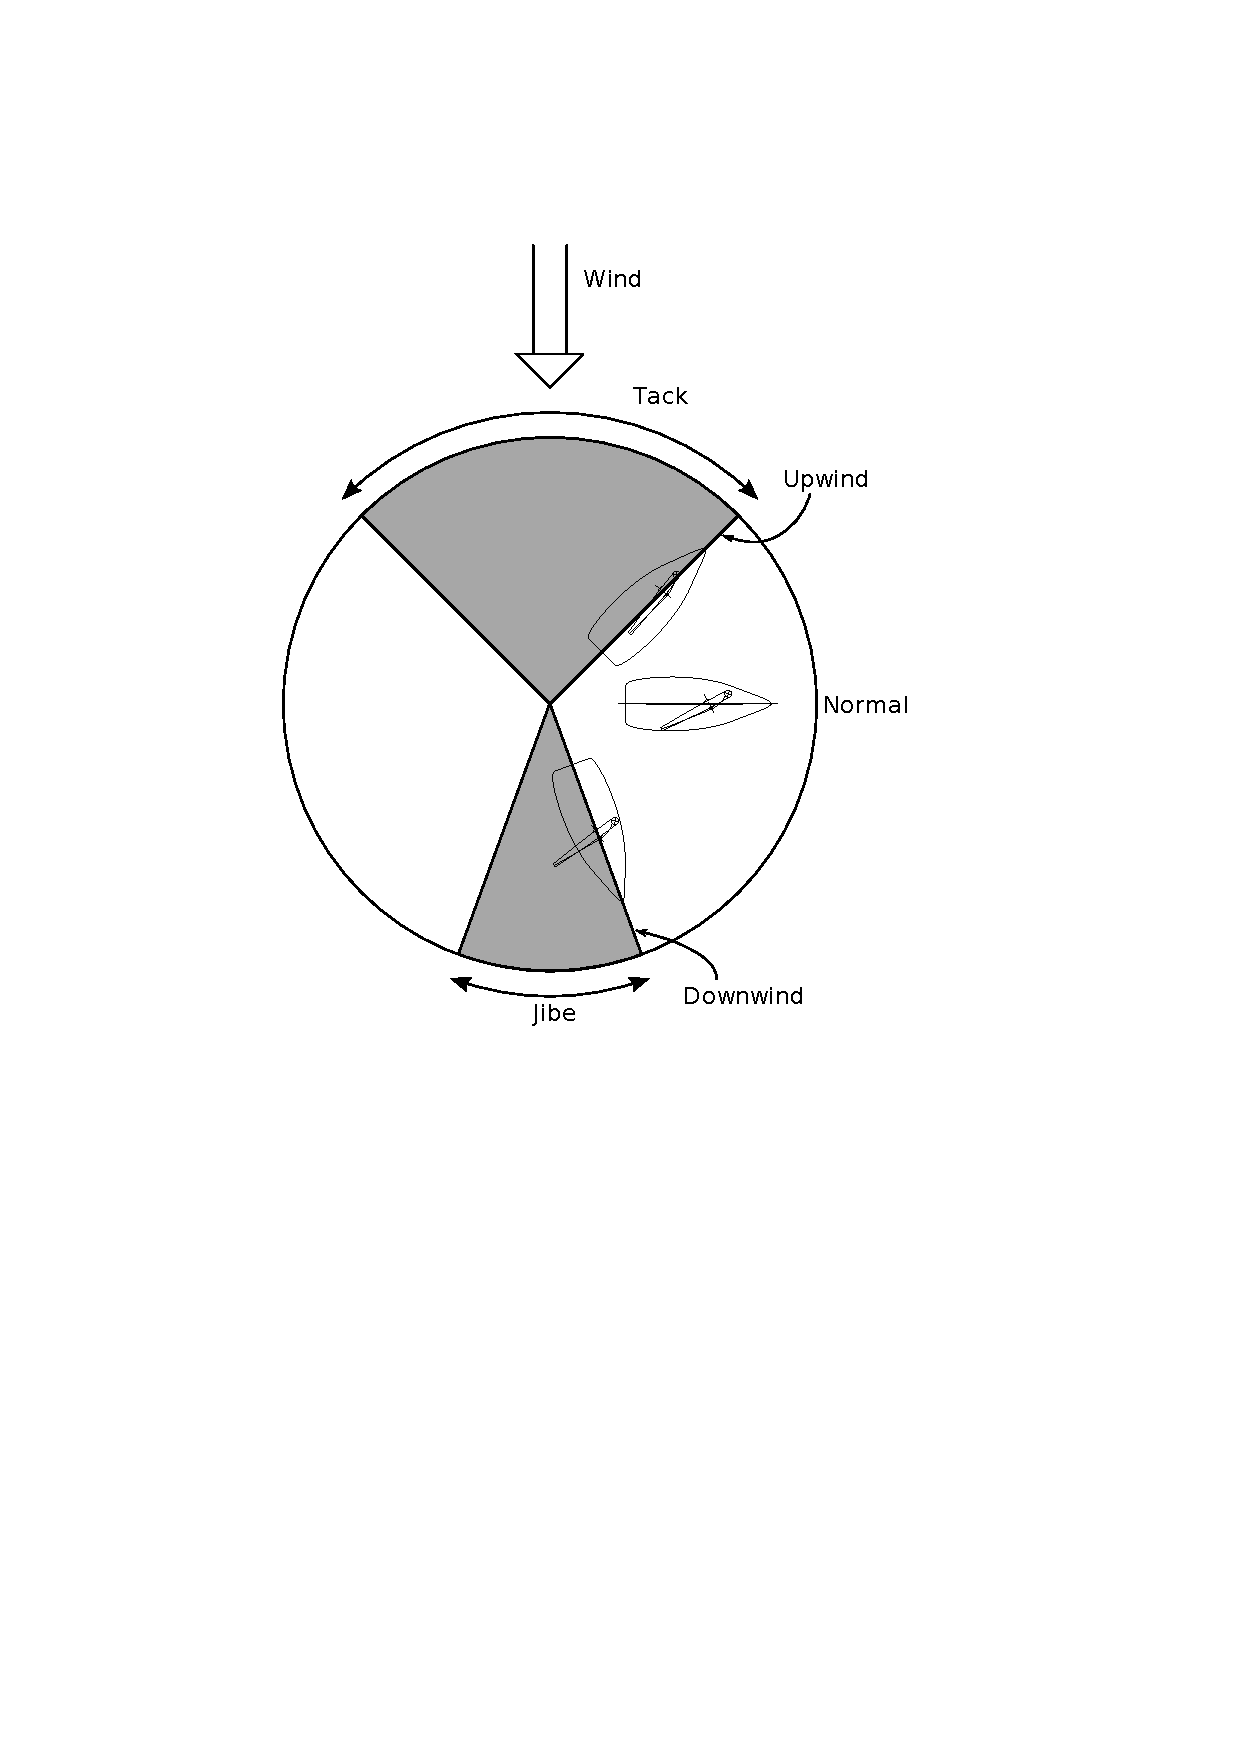
\includegraphics[trim = 45mm 120mm 55mm 45mm, clip, width=0.70\columnwidth]{pics/courses_to_wind.pdf}
\caption{Possible courses of a sailing yacht with respect to the wind and corresponding control system states. The range with wind directly from behind could be sailed in theory, but is not very efficient and rather unstable.}\label{fig:courses_to_wind}
\end{figure}
\subsubsection{Normal Sailing}
If the desired heading given by the path planner (section \ref{sec:navigator}) is
in the sailable (white) range, the system is in state \texttt{Normal Sailing}.
In this state the rudder controller follows the given desired heading, while
the sail controller permanently adjusts the sail to achieve the optimal angle
of attack on the sail. If the desired heading changes within the sailable
range, the rudder controller simply follows the new course while the sail
controller maintains a constant angle of attack.
\subsubsection{Upwind Sailing}
If the desired heading for whatever reason is set in the not sailable (gray)
range, it cannot be directly followed. The objective in this case is to make as
much velocity towards the wind as possible. In \texttt{Upwind Sailing} mode the
sail is set to the tightest position that is reasonably possible. While the
sail angle is kept at this constant position, the rudder controller now keeps a
constant heading angle to the true wind and thus takes advantage of all wind shifts.
Note that the behaviour is similar for downwind sailing.
%
\subsection{Test Results and Analysis} \label{sec:sailor_testing}
Several tests were undertaken to verify and optimise the control system. Before
any testing on the water was done, the state machine's transition conditions
had to be verified. This was done by putting the boat on a trailer on a
sufficiently windy day and turning it around its vertical axis while constantly
checking the current state. We encountered many problems that were caused by
the sign change between $-180^o$ and $+180^o$. Some time could have been saved,
if the whole control program, including the state machine, had been tested more
thoroughly in the simulation environment.

The controller was then tested for its ability to keep a desired heading and to
react to changes in desired heading. After some tuning of the PID parameters we
found that the parameters in table \ref{tab:pid_params} yield fast reactions
without too much overshoot.
%
\begin{table}[htb]
\caption{PID Parameters} \label{tab:pid_params}
\centering
\begin{tabular}{c|l}\hline
P & 0.3  \\ \hline
I & 0.005 \\ \hline
D & 30 \\ \hline
\end{tabular}
\end{table}
%
A step response in winds of about 20 knots is illustrated in figure
\ref{fig:step_response_wind20kn}. Note that 20 knots is already a strong wind
and that in lower wind speeds we experienced much less oscillation around the
reference value. Even this $\pm 10^o$ oscillation that is mostly caused by
waves can barely be seen on the boat. We then also applied disturbances to the
boat by deviating it from its course by hand. The reaction was the same as with
changes in desired heading.
%
\begin{figure}[thb]
\centering
% trim = left bottom right top
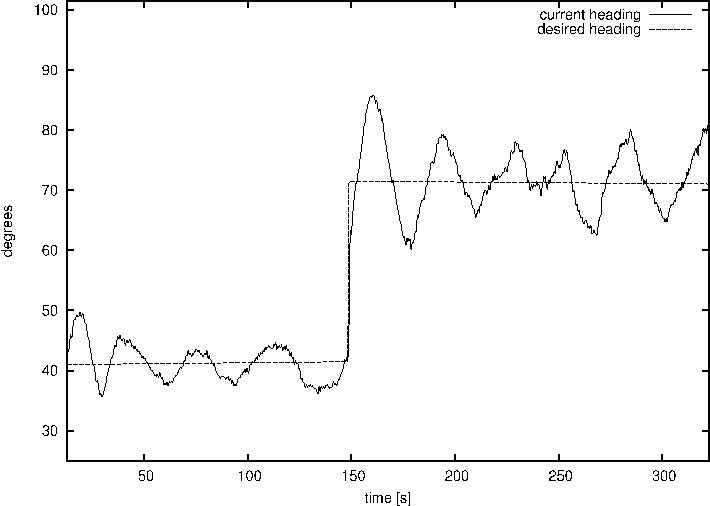
\includegraphics[trim = 0mm 0mm 0mm 0mm, clip, width=7cm]{pics/reference_step_usee4_2.pdf}
\caption{Step response in state \texttt{Normal Sailing}. Conditions were 20\,kn wind from 140°}\label{fig:step_response_wind20kn}
\end{figure}

Figure \ref{fig:3tacks_upwind_sailing} shows current heading, desired heading
and wind direction during three tacks. Between the tacks, the controller state
machine is in state \texttt{Upwind Sailing}. It can be very well seen, that the
boat keeps a constant angle to the wind and takes advantage of wind shifts as
expected.
\begin{figure}[thb]
\centering
% trim = left bottom right top
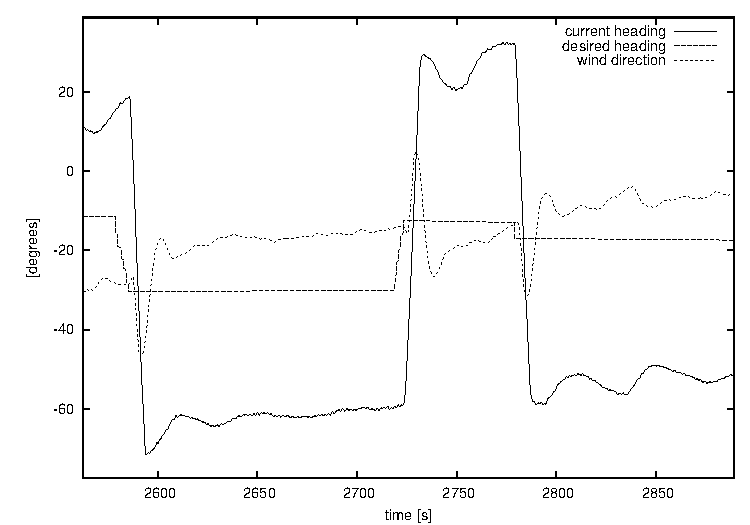
\includegraphics[trim = 0mm 0mm 0mm 0mm, clip, width=7cm]{pics/tacks_to_upwind_usee5_wind8kn_hdg.pdf}
\caption{3 tacks, with \texttt{Upwind Sailing} in between.}\label{fig:3tacks_upwind_sailing}
\end{figure}
A lot of time was invested into correct timing during tack and jibe. In the
beginning we had several problems that resulted in inappropriate sail tuning
during or right after manoeuvres. This sometimes even resulted in the boat
sailing backwards.

Figure \ref{fig:wyp_autonom_drift_comp} shows how the boat follows a trajectory
that was calculated by the path planner. The path planner's calculation was started
at the bottom left where the dashed line begins. After the calculation was
completed, the boat jibes and sets the new course. After a few seconds the
drift compensation starts to work and the boat's real course approaches the
desired trajectory.
%
\begin{figure}[thb]
\centering
% trim = left bottom right top
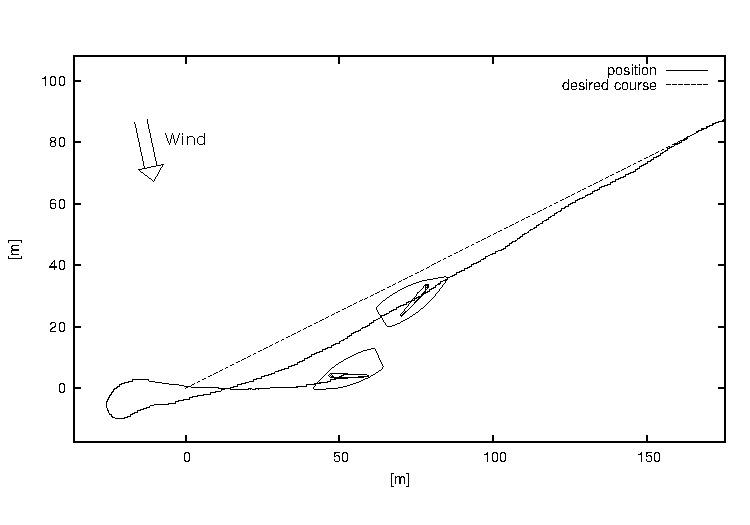
\includegraphics[trim = 0mm 0mm 0mm 0mm, clip, width=7cm]{pics/driftcompensation.pdf}
\caption{GPS plot of the controller following a desired trajectory calculated
by the path planner. It was recorded during a test on the Urnersee in about 15
knots wind.}\label{fig:wyp_autonom_drift_comp}
\end{figure}


\section{Path Planner} \label{sec:navigator}
\subsection{Principle of motion planning for a sailing boat} \label{sec:intro_principle}
Due to the nature of every sailing vessel, \textsc{Avalon}'s manoeuvrability is
limited in relation to wind direction. Additionally, due to the non-holonomic
properties of a sailing vessel, it is not possible to change the heading on the
spot immediately.  The trajectory tracker (see section \ref{sec:skipper}) has
to keep that in mind and operate in a way that allows a certain space to make
heading changes. For the implementation of a navigation algorithm, these
constraints imply that using accurate wind information for every calculation is
essential.
 
\subsection{Literature Research}
%
Path planning in the naval industry is not a new topic. For many years,
commercial ships have used weather forecasts to generate an optimal path with
respect to speed or bypassing bad weather situations. For sailing ships,
commercial solutions by companies like \textsc{B \& G} or \textsc{Northstar}
exist, but do not offer any possibility to be integrated into our embedded
system. Looking at different navigation and routing strategies, two
fundamentally different ideas emerge: Roland Stelzer \cite{stelzer2008}, who
has published his approach also for implementation in an autonomous sailing
boat, projects the speed vector on the target direction and tries to find a
sailable heading that maximises that projected speed vector. Although in small
scale it might find a good and fast path, this approach is not sufficient when
it comes to larger search areas with obstacles and additional inputs like
weather forecasts.

The other approach is to use grid based path planning algorithms that allow us
to generate optimal solutions considering the path from start to goal and
enable the integration of specific constraints (see section
\ref{sec:intro_principle}).

\textit{Breadth first method} and \textit{Depth first} are both based on a very
simple principle and serve as archetypes for many important algorithms
\cite{cormen2001}, but may result in very long running time. \textit{Dijkstra}
on the other hand is a directed search \cite{lavalle2006} and guarantees
optimal results. A* is a modified version of \textit{Dijkstra} that also
considers the heuristic distance estimate of the path from current position to
the destination \cite{hart1968}, which makes it more directed than
\textit{Dijkstra}. One of the problems of grid-based planning algorithms is
that the angles are artificially constrained. The Theta*-Algorithm
\cite{nash2007} deals with that handicap and produces more realistic looking
paths than A* or even smoothed A*. A further extension of A* is D*
\cite{stentz1995}, which incorporates dynamic changes (i. e. moving obstacles)
along the path and does not require to replan the whole path from current
position to destination anymore.

The proposed approach uses a simple A* algorithm which is modified to comply
with all the sailing constraints. It must also be noted that there is few
computation time constraints for a sailing boat crossing the Atlantic ocean.
Even if path planning requires a handful of minutes, this is still an
acceptable behaviour.
%
\subsection{Planning Strategy}
%
Considering the distance of about 4'200 nautical miles \textsc{Avalon} has to
sail on its journey across the Atlantic Ocean and its slow speed of
about 4 to 5 knots\footnote{1 knot is 1 nautical mile per hour}, it is essential to distinguish between a global and a local
planning. Global planning will be done by fixing way-points across the Atlantic
based on expert knowledge, weather and current analysis. The local planner will
then plan from current position to the next global way-point using wind data
from the on board sensor. The planning algorithm will be triggered and
controlled by a trajectory tracker (section \ref{sec:skipper}), which knows
exactly towards which way-point \textsc{Avalon} is sailing at the moment.
%
\subsection{Interfaces with the controller}
An important part of the software structure is the interface between the
navigation program and the control system (see section \ref{sec:sailor}). The main
reason why we decided to pass \textit{headings} instead of way-points from the
planner via the trajectory tracker to the controller, was that the planner calculates an optimal
path with respect to path duration for specific angles to the wind.
Drift that pushes the vessel off the trajectory will be handled by the controller,
a new calculation will only take place after the boat has a certain deviation
from the set trajectory (see section \ref{sec:skipper}).
\paragraph{Wind data}
The wind the local path planner uses is an average of the measurements over the last 90 seconds. The control system will then follow the received desired heading using a much more accurate wind direction that was averaged only over a period of 5 seconds (see section \ref{sec:sailor}). Figure \ref{fig:cleanwind} shows a comparison of the two different wind sets.
%
\begin{figure}
 \centering
 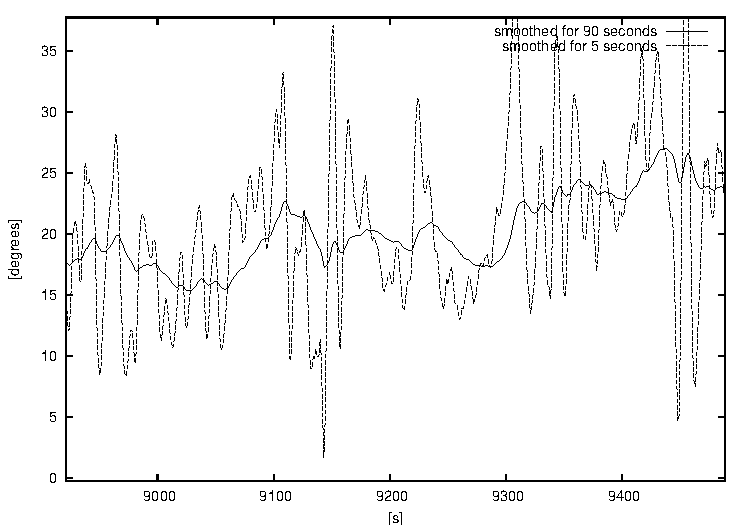
\includegraphics[width = 6.5 cm]{pics/paper_cleanwind.pdf}
 \caption{Differently filtered wind information}
 \label{fig:cleanwind}
\end{figure}

%
\subsection{Planning algorithm}
As explained earlier, \textit{Dijkstra}'s graph search is the basic algorithm
used to perform the path search. Starting at an initial grid-point, the algorithm expands over the whole field until the final grid-point has been reached. Every evaluated grid-point will be assigned a certain cost, a time estimate of how long it will take the boat to sail from the initial grid-point to the point that is currently being evaluated. The final optimal path is then determined by always following the neighbor with the lowest costs from the final to the initial grid-point. 

To be able to allocate costs for ship movements, i. e. moving from one grid-point to a neighbor, we work in 3 dimensions, with $x$ and $y$ for the geographic position
and $\theta$ for the heading of the boat at that position. To get sailable and
reasonable results, the following costs have been implemented additionally:
%
\begin{itemize}
\item Sailing-Time from start node
\item Estimated sailing time to the end node (heuristic)
\item Cost for heading changes
\item Cost for manoeuvres (tack and jibe)
\item Cost for offset from the straight connection between start and end node (tunnel cost).
\end{itemize}
%
\subsubsection{Grid compatible coordinate system}
To represent GPS points on a map, a coordinate transformation is necessary. Since we plan only for short distances ahead of us (local planning), we can use a very simplified transformation into meter coordinates 
\begin{equation}
\begin{array}{l}
 x = R_E \cdot \cos\left( \text{lat}\right) \cdot \dfrac{\pi}{180\, deg} \cdot \text{lon}\\
\\
 y = R_E \cdot\dfrac{\pi}{180\, deg}\cdot \text{lat}
\end{array}
\end{equation}
where $R_E$ is the earth radius, lon and lat the GPS coordinates in degrees. This transformation assumes a flat water surface \cite{stelzer2008}. In order to initialise the local map as small as possible, the algorithm places the origin as close as possible to either start or target coordinate. 
%
\subsubsection{Polar diagram}
In order to calculate the boat speed for a specific angle to the wind, a polar
diagram\footnote{In boating term, the polar diagram gives a boat velocity  as a
function of its  heading to the wind and the wind velocity} of \textsc{Avalon}
is needed.  Since creating a detailed diagram for our boat would require
constant wind and wave conditions over a long time, we created a polar diagram
based on existing diagrams for bigger vessels. Testing has shown that we get
reasonable results by restricting the sailable \textit{angle to the wind} to
the area between $45^o$ and $160^o$ (see figure \ref{fig:courses_to_wind}).
%
\subsubsection{Heading}
\hide{
% This is too much inmplementation dependent
We assume a 24 neighbour grid throughout this paper, which allows to have
sixteen different headings available for sailing. Another advantage of being
able to expand to the second but next neighbour-grid is the fact that it reduces
the number of way-points, since one grid node is skipped.
\subsubsection{Connectivity List}
In theory, every heading change is possible with a sailing boat. However, to
make the algorithm faster, we have constricted the biggest possible change of
heading to $90^o$. The areas that are not sailable due to the wind direction
are between $\pm45^o$ to wind direction for sailing upwind and $\pm160^o$ to
wind direction for sailing downwind (see figure \ref{fig:courses_to_wind}).
%
}
In order to limit the size of the 3D grid used in this paper, we use a
discretisation of the possible boat heading into 16 possible headings. In usual
2D grid-based path planning, transition from one cell to its 8 neighbours is
considered. This results in only 8 possible changes of orientation. By
considering a neighbourhood of 24 cells (8 cells around the starting cell, plus
16 cells one cell further), we can reach 16 different heading changes in one
transition. This leads to smoother paths and smaller number of way-points on the
final path.

We further reduce the computational complexity of the planner by considering
that the maximum change of heading in one transition is $90^o$. This
restriction is consistent with the experience of human skippers. 
%
\subsection{Cost Factors}
\subsubsection{General Costs}
The general aim of this algorithm is to find the shortest path for a sailing vessel to go from point $A$ to point $B$. The general cost we give for every movement is therefore \textit{sailing time to the next node}, calculated by equation \ref{eq:navi_timecost}. The speed solely depends on the angle to the wind and the wind speed. 
\begin{equation}
 \text{sailing time} = \frac{\text{distance to next node}}{\text{speed}} 
\label{eq:navi_timecost}
\end{equation}
\subsubsection{Heuristic Estimate}
The heuristic estimate is used to evaluate the remaining time to the goal.
According to \cite{lavalle2006}, the only constraint on the heuristic is that
it has to underestimate the real cost of the remaining path. For simplicity sake, the
heuristic returns the time it would take to sail to the goal at an exaggerated speed of 10 knots. More complicated options have been considered, but none of them provided well defined behaviour in all situations.

\subsubsection{Turning Cost}
To generate paths as smooth as possible, the algorithm places costs $C_{\text{new}}$ for heading changes, using a simple linear factor $f$ in equation
\begin{equation}
 C_{\text{new}} = f \cdot \vert \theta_{\text{curr}} - \theta_{\text{new}} \vert  
\label{eq:navi_turningcost}
\end{equation}
where $\theta_{\text{curr}}$ and $\theta_{\text{new}}$ are the respective headings. 
%
\subsubsection{Cost for Tack or Jibe}
By giving a certain cost for tack or jibe, we can indirectly control the number
of manoeuvres \textsc{Avalon} sails.  The principle is very simple, we check if
the sign of $(\theta_{\text{curr}} - \text{winddirection})$ and $(\theta_{\text{next}} -
\text{winddirection})$ is the same. If it is different, an additional cost will be
added to the total cost.
%
\subsubsection{Tunnel cost}
In order to favour paths that stay closer to the straight line path, we
allocate costs increasing with the distance from the direct connection of start
and target node. It has proved best to increase the cost only little for the
areas in the middle of the tunnel but increase it abruptly when closing in on
the borders. 
%
\subsubsection{Obstacle avoidance} 
To avoid islands and coastal regions, the algorithm gives extremely high costs
for passing prohibited terrain. To locate these areas, it parses information
from a map.\\
To avoid commercial ships on the Atlantic, \textsc{Avalon} can receive AIS
signals from most ships travelling over the Atlantic. Knowing ship speed,
direction and current position, our algorithm will place no-go areas around potential collision locations to make sure to bypass them.
%
% we had that already in chapter nav_strategy:
\hide{
\subsection{Trajectory tracker} \label{sec:skipper}
The trajectory tracker has mainly two important tasks:
\begin{itemize}
 \item Triggering the local planner
 \item Calculating a desired heading for the control system
\end{itemize}
\subsubsection{State machine}
To manage the different tasks, the trajectory tracker can switch between different states:
%
\paragraph{Standard Navigation}
If not approaching a target or buoy, this state generates headings for the control system, going from way-point to way-point.
If the wind changes more than $20$° or if the ship distances itself from the current trajectory for more than a predefined distance, a new calculation will be initiated. 
\paragraph{Goal Approach}
If approaching a target position, the trajectory tracker will always send a heading that is directing exactly towards that point.
\paragraph{Buoy Approach}
This is a state designed especially for short course racing. Due to regulations that always require a port-side surrounding of the regatta buoys, this state will - when approaching a buoy - always write a heading that will lead the boat around the buoy.
\paragraph{New Calculation}
In this state, the trajectory tracker manages and supervises the new calculation. After having checked that the new way-points have been stored, it switches back to \textit{Standard Navigation}
}
%
%
\subsection{Tests and Discussion}
\subsubsection{Testing environment}
Most tests and parameter optimization was done by visualising the generated
path on screen and discussing its quality. Figure \ref{fig:navi_path}
shows two calculated path examples, both having to pass an obstacle and dealing
with difficult wind direction like upwind and downwind. Analysis has shown that the addition of a tunnel cost is redundant since the heuristic estimate also favours paths that are close to the direct connection of {\em start} and {\em target} node. Although adding an artificial tunnel cost might not always result in optimal path solutions, we used the tunnel for safety reasons to make sure that the vessel never sails beyond predefined boundaries. 
\hide{
% In case of present obtacles, this is not always optimal.
\paragraph{Initial and final Heading}
Our initial motion was to set the current boat heading as $theta$ at the START
node. In case the TARGET was exactly in the opposite direction, the algorithm
then proposed a turn, which took about two to three way-points. Tests on the
water showed that this was not optimal at all and the manoeuvre cost us a lot of
time. We then set the START $theta$ directly towards the TARGET, which produced
much better results. One disadvantage is that the boat might sail away too far
from the starting point in case of long calculation time without receiving the
new heading. After calculation has finished, the trajectory tracker would then
notice the incoherence and trigger a new calculation. 
}

Another important and not yet solved problem is the final heading at the target
node that has to be known in order for \textit{Dijkstra} to start the search. At the
moment the algorithm chooses a final heading that is as close as possible to
the direct heading of a straight line from start to destination but always
differs at minimum $45^o$ from the wind direction. This usually produces good
results but it does not take obstacles into account which means that sometimes
an additional, unnecessary turn is produced. 

In practice, this issue will be solved by starting planning a new path before
completing the execution of the current one.


\begin{figure}[htb]
  \centering
  \subfloat[Upwind]{\label{fig:navi_upwind}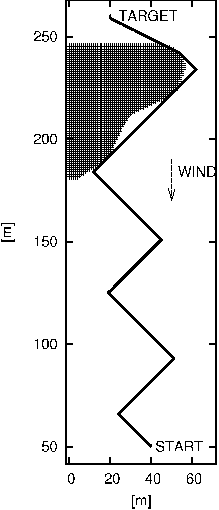
\includegraphics[width=2.7 cm]{pics/paper_kreuzen2.pdf}} 
  \hspace{1cm}
  \subfloat[Downwind]{\label{fig:navi_downwind}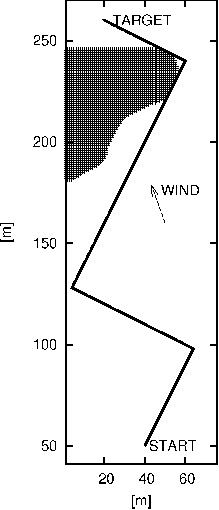
\includegraphics[width=2.7 cm]{pics/paper_downwind2.pdf}}
  \caption{Path examples for upwind and downwind sailing with obstacles}
  \label{fig:navi_path}
\end{figure}

\begin{figure}[htb]
\centering
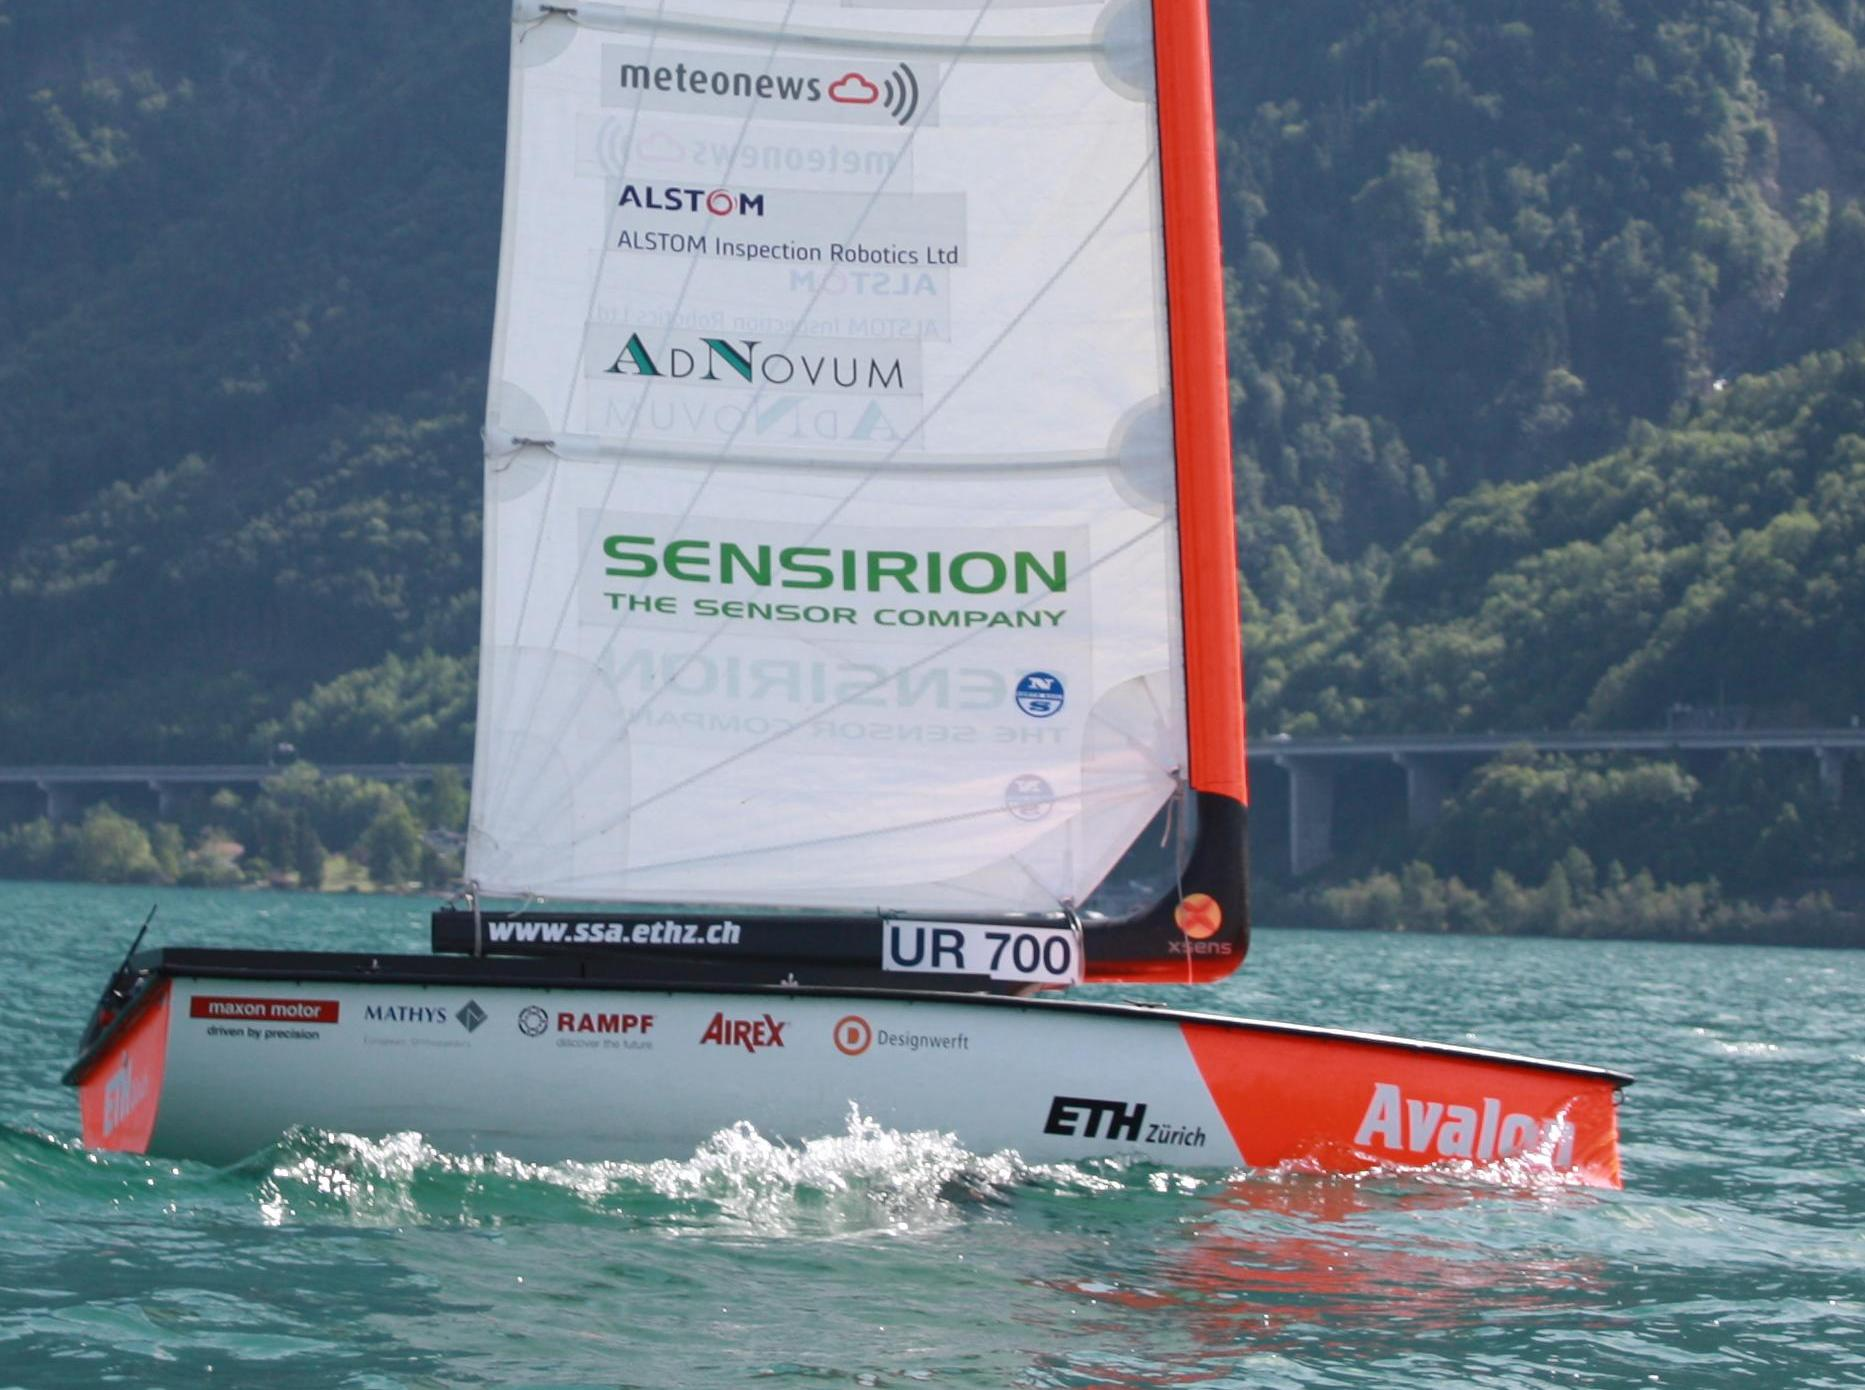
\includegraphics[width=0.75\columnwidth]{pics/IMG_0601_papercrop.jpeg}
\caption{Avalon during testing in high winds}
%\label{fig:avalon}
\end{figure}

\section{Conclusion and Outlook}
The proposed navigation and control software has been successfully implemented
in our autonomous sailboat \textsc{Avalon}. Several short-run tests both on
Swiss lakes and on the Atlantic Ocean have been carried out and have shown that the
described control and navigation system work. \textsc{Avalon} was exposed to
wind conditions ranging from almost 0 to 30 knots. The experimentally found
control parameters have proven to be well defined, keeping the vessel on course
even while sailing in rough sea states.

In very low wind speeds it was seen that the boat is able to sail much better
by itself than steered by us via remote control, because it is always aware of
the exact wind direction, even when human sailors hardly notice any wind at
all.

However, especially in reference to a possible crossing of the Atlantic Ocean,
several tests over a bigger period of time as well as longer distances have to
be performed in a next stage. 

By processing received AIS-signals, \textsc{Avalon} is able to identify other
ships in close proximity and therefore prevent collisions. However, small boats
that don't send position information cannot be recognized at this stage and
further research has to be done in identifying obstacles visually.   

Implementing a conventional and proved path planner like Dijkstra's for our
navigation system has proved well. Visually and analytically evaluated results
show that we achieve better solutions by taking the whole path into account
than by always optimising the heading at every current position. However, by
adding additional costs (like tunnel cost), optimal path solutions are not
always guaranteed.

Our goal for future work is to further optimise the software, especially
regarding energy consumption. For example a hysteresis could be added to the
sail tuner so that the sail does not constantly adapt to minor changes in wind
direction and speed. A further area of improvement could be in making use of
weather forecasts in the global navigation. For our boat this does not add much
value, because it is too slow to react to forecast weather changes.


% can use a bibliography generated by BibTeX as a .bbl file
% BibTeX documentation can be easily obtained at:
% http://www.ctan.org/tex-archive/biblio/bibtex/contrib/doc/
% The IEEEtran BibTeX style support page is at:
% http://www.michaelshell.org/tex/ieeetran/bibtex/
\bibliographystyle{IEEEtran}
\bibliography{IEEEabrv,ram_paper_ssa}

%

% Note that the a4paper option is mainly intended so that authors in
% countries using A4 can easily print to A4 and see how their papers will
% look in print - the typesetting of the document will not typically be
% affected with changes in paper size (but the bottom and side margins will).
% Use the testflow package mentioned above to verify correct handling of
% both paper sizes by the user's LaTeX system.
%
% Also note that the "draftcls" or "draftclsnofoot", not "draft", option
% should be used if it is desired that the figures are to be displayed in
% draft mode.
%
\documentclass[journal,final,letterpaper,twoside,twocolumn]{IEEEtran}
%\documentclass[journal,final,letterpaper,twoside,twocolumn]{IEEEtran}
% Add the compsoc option for Computer Society conferences.
%
% If IEEEtran.cls has not been installed into the LaTeX system files,
% manually specify the path to it like:
% \documentclass[conference]{../sty/IEEEtran}

\usepackage[utf8]{inputenc}        % Keybord settings


% Some very useful LaTeX packages include:
% (uncomment the ones you want to load)


% *** MISC UTILITY PACKAGES ***
%
%\usepackage{ifpdf}
% Heiko Oberdiek's ifpdf.sty is very useful if you need conditional
% compilation based on whether the output is pdf or dvi.
% usage:
% \ifpdf
%   % pdf code
% \else
%   % dvi code
% \fi
% The latest version of ifpdf.sty can be obtained from:
% http://www.ctan.org/tex-archive/macros/latex/contrib/oberdiek/
% Also, note that IEEEtran.cls V1.7 and later provides a builtin
% \ifCLASSINFOpdf conditional that works the same way.
% When switching from latex to pdflatex and vice-versa, the compiler may
% have to be run twice to clear warning/error messages.






% *** CITATION PACKAGES ***
%
\usepackage{cite}
\usepackage{textcomp}

% cite.sty was written by Donald Arseneau
% V1.6 and later of IEEEtran pre-defines the format of the cite.sty package
% \cite{} output to follow that of IEEE. Loading the cite package will
% result in citation numbers being automatically sorted and properly
% "compressed/ranged". e.g., [1], [9], [2], [7], [5], [6] without using
% cite.sty will become [1], [2], [5]--[7], [9] using cite.sty. cite.sty's
% \cite will automatically add leading space, if needed. Use cite.sty's
% noadjust option (cite.sty V3.8 and later) if you want to turn this off.
% cite.sty is already installed on most LaTeX systems. Be sure and use
% version 4.0 (2003-05-27) and later if using hyperref.sty. cite.sty does
% not currently provide for hyperlinked citations.
% The latest version can be obtained at:
% http://www.ctan.org/tex-archive/macros/latex/contrib/cite/
% The documentation is contained in the cite.sty file itself.






% *** GRAPHICS RELATED PACKAGES ***
%
\ifCLASSINFOpdf
  \usepackage[pdftex]{graphicx}
  % declare the path(s) where your graphic files are
  % \graphicspath{{../pdf/}{../jpeg/}}
  % and their extensions so you won't have to specify these with
  % every instance of \includegraphics
  % \DeclareGraphicsExtensions{.pdf,.jpeg,.png}
\else
  % or other class option (dvipsone, dvipdf, if not using dvips). graphicx
  % will default to the driver specified in the system graphics.cfg if no
  % driver is specified.
 \usepackage[dvips]{graphicx}
  % declare the path(s) where your graphic files are
  % \graphicspath{{../eps/}}
  % and their extensions so you won't have to specify these with
  % every instance of \includegraphics
  % \DeclareGraphicsExtensions{.eps}
\fi
% graphicx was written by David Carlisle and Sebastian Rahtz. It is
% required if you want graphics, photos, etc. graphicx.sty is already
% installed on most LaTeX systems. The latest version and documentation can
% be obtained at:
% http://www.ctan.org/tex-archive/macros/latex/required/graphics/
% Another good source of documentation is "Using Imported Graphics in
% LaTeX2e" by Keith Reckdahl which can be found as epslatex.ps or
% epslatex.pdf at: http://www.ctan.org/tex-archive/info/
%
% latex, and pdflatex in dvi mode, support graphics in encapsulated
% postscript (.eps) format. pdflatex in pdf mode supports graphics
% in .pdf, .jpeg, .png and .mps (metapost) formats. Users should ensure
% that all non-photo figures use a vector format (.eps, .pdf, .mps) and
% not a bitmapped formats (.jpeg, .png). IEEE frowns on bitmapped formats
% which can result in "jaggedy"/blurry rendering of lines and letters as
% well as large increases in file sizes.
%
% You can find documentation about the pdfTeX application at:
% http://www.tug.org/applications/pdftex





% *** MATH PACKAGES ***
%
\usepackage[cmex10]{amsmath}
% A popular package from the American Mathematical Society that provides
% many useful and powerful commands for dealing with mathematics. If using
% it, be sure to load this package with the cmex10 option to ensure that
% only type 1 fonts will utilized at all point sizes. Without this option,
% it is possible that some math symbols, particularly those within
% footnotes, will be rendered in bitmap form which will result in a
% document that can not be IEEE Xplore compliant!
%
% Also, note that the amsmath package sets \interdisplaylinepenalty to 10000
% thus preventing page breaks from occurring within multiline equations. Use:
%\interdisplaylinepenalty=2500
% after loading amsmath to restore such page breaks as IEEEtran.cls normally
% does. amsmath.sty is already installed on most LaTeX systems. The latest
% version and documentation can be obtained at:
% http://www.ctan.org/tex-archive/macros/latex/required/amslatex/math/





% *** SPECIALIZED LIST PACKAGES ***
%
%\usepackage{algorithmic}
% algorithmic.sty was written by Peter Williams and Rogerio Brito.
% This package provides an algorithmic environment fo describing algorithms.
% You can use the algorithmic environment in-text or within a figure
% environment to provide for a floating algorithm. Do NOT use the algorithm
% floating environment provided by algorithm.sty (by the same authors) or
% algorithm2e.sty (by Christophe Fiorio) as IEEE does not use dedicated
% algorithm float types and packages that provide these will not provide
% correct IEEE style captions. The latest version and documentation of
% algorithmic.sty can be obtained at:
% http://www.ctan.org/tex-archive/macros/latex/contrib/algorithms/
% There is also a support site at:
% http://algorithms.berlios.de/index.html
% Also of interest may be the (relatively newer and more customizable)
% algorithmicx.sty package by Szasz Janos:
% http://www.ctan.org/tex-archive/macros/latex/contrib/algorithmicx/




% *** ALIGNMENT PACKAGES ***
%
%\usepackage{array}
% Frank Mittelbach's and David Carlisle's array.sty patches and improves
% the standard LaTeX2e array and tabular environments to provide better
% appearance and additional user controls. As the default LaTeX2e table
% generation code is lacking to the point of almost being broken with
% respect to the quality of the end results, all users are strongly
% advised to use an enhanced (at the very least that provided by array.sty)
% set of table tools. array.sty is already installed on most systems. The
% latest version and documentation can be obtained at:
% http://www.ctan.org/tex-archive/macros/latex/required/tools/


%\usepackage{mdwmath}
%\usepackage{mdwtab}
% Also highly recommended is Mark Wooding's extremely powerful MDW tools,
% especially mdwmath.sty and mdwtab.sty which are used to format equations
% and tables, respectively. The MDWtools set is already installed on most
% LaTeX systems. The lastest version and documentation is available at:
% http://www.ctan.org/tex-archive/macros/latex/contrib/mdwtools/


% IEEEtran contains the IEEEeqnarray family of commands that can be used to
% generate multiline equations as well as matrices, tables, etc., of high
% quality.


%\usepackage{eqparbox}
% Also of notable interest is Scott Pakin's eqparbox package for creating
% (automatically sized) equal width boxes - aka "natural width parboxes".
% Available at:
% http://www.ctan.org/tex-archive/macros/latex/contrib/eqparbox/





% *** SUBFIGURE PACKAGES ***
%\usepackage[tight,footnotesize]{subfig}
% subfigure.sty was written by Steven Douglas Cochran. This package makes it
% easy to put subfigures in your figures. e.g., "Figure 1a and 1b". For IEEE
% work, it is a good idea to load it with the tight package option to reduce
% the amount of white space around the subfigures. subfigure.sty is already
% installed on most LaTeX systems. The latest version and documentation can
% be obtained at:
% http://www.ctan.org/tex-archive/obsolete/macros/latex/contrib/subfigure/
% subfigure.sty has been superceeded by subfig.sty.



\usepackage[caption=false]{caption}
\usepackage[font=footnotesize]{subfig}
% subfig.sty, also written by Steven Douglas Cochran, is the modern
% replacement for subfigure.sty. However, subfig.sty requires and
% automatically loads Axel Sommerfeldt's caption.sty which will override
% IEEEtran.cls handling of captions and this will result in nonIEEE style
% figure/table captions. To prevent this problem, be sure and preload
% caption.sty with its "caption=false" package option. This is will preserve
% IEEEtran.cls handing of captions. Version 1.3 (2005/06/28) and later
% (recommended due to many improvements over 1.2) of subfig.sty supports
% the caption=false option directly:
%\usepackage[caption=false,font=footnotesize]{subfig}
%
% The latest version and documentation can be obtained at:
% http://www.ctan.org/tex-archive/macros/latex/contrib/subfig/
% The latest version and documentation of caption.sty can be obtained at:
% http://www.ctan.org/tex-archive/macros/latex/contrib/caption/




% *** FLOAT PACKAGES ***
%
%\usepackage{fixltx2e}
% fixltx2e, the successor to the earlier fix2col.sty, was written by
% Frank Mittelbach and David Carlisle. This package corrects a few problems
% in the LaTeX2e kernel, the most notable of which is that in current
% LaTeX2e releases, the ordering of single and double column floats is not
% guaranteed to be preserved. Thus, an unpatched LaTeX2e can allow a
% single column figure to be placed prior to an earlier double column
% figure. The latest version and documentation can be found at:
% http://www.ctan.org/tex-archive/macros/latex/base/



%\usepackage{stfloats}
% stfloats.sty was written by Sigitas Tolusis. This package gives LaTeX2e
% the ability to do double column floats at the bottom of the page as well
% as the top. (e.g., "\begin{figure*}[!b]" is not normally possible in
% LaTeX2e). It also provides a command:
%\fnbelowfloat
% to enable the placement of footnotes below bottom floats (the standard
% LaTeX2e kernel puts them above bottom floats). This is an invasive package
% which rewrites many portions of the LaTeX2e float routines. It may not work
% with other packages that modify the LaTeX2e float routines. The latest
% version and documentation can be obtained at:
% http://www.ctan.org/tex-archive/macros/latex/contrib/sttools/
% Documentation is contained in the stfloats.sty comments as well as in the
% presfull.pdf file. Do not use the stfloats baselinefloat ability as IEEE
% does not allow \baselineskip to stretch. Authors submitting work to the
% IEEE should note that IEEE rarely uses double column equations and
% that authors should try to avoid such use. Do not be tempted to use the
% cuted.sty or midfloat.sty packages (also by Sigitas Tolusis) as IEEE does
% not format its papers in such ways.




% *** PDF, URL AND HYPERLINK PACKAGES ***
%
%\usepackage{url}
% url.sty was written by Donald Arseneau. It provides better support for
% handling and breaking URLs. url.sty is already installed on most LaTeX
% systems. The latest version can be obtained at:
% http://www.ctan.org/tex-archive/macros/latex/contrib/misc/
% Read the url.sty source comments for usage information. Basically,
% \url{my_url_here}.





% *** Do not adjust lengths that control margins, column widths, etc. ***
% *** Do not use packages that alter fonts (such as pslatex).         ***
% There should be no need to do such things with IEEEtran.cls V1.6 and later.
% (Unless specifically asked to do so by the journal or conference you plan
% to submit to, of course. )


% correct bad hyphenation here
\hyphenation{op-tical net-works semi-conduc-tor middle-ware}

\newcommand{\hide}[1]{}
\begin{document}
%
% paper title
% can use linebreaks \\ within to get better formatting as desired
\title{Navigation Strategy and Trajectory Following Controller for an Autonomous Sailing Vessel}



% author names and affiliations
% use a multiple column layout for up to three different
% affiliations



%\author{

%\IEEEauthorblockN{Sebastian Boehl\IEEEauthorrefmark{1}}

%\and

%\IEEEauthorblockN{Lian P. Giger}
%\IEEEauthorblockA{ETH\\Federal Institute of Technology\\
%Zurich, Switzerland\\
%Email: ligiger@student.ethz.ch}

%\and

%\IEEEauthorblockN{Stefan Wismer} \IEEEauthorblockA{ETH Zurich}}

% conference papers do not typically use \thanks and this command
% is locked out in conference mode. If really needed, such as for
% the acknowledgment of grants, issue a \IEEEoverridecommandlockouts
% after \documentclass

% for over three affiliations, or if they all won't fit within the width
% of the page, use this alternative format:
%
\author{\IEEEauthorblockN{Hendrik Erckens ({\small corresponding author}), Gion-Andri Büsser,\\Dr. C\'{e}dric Pradalier, Prof Dr. Roland Y. Siegwart\\ \IEEEauthorblockA{Autonomous Systems Lab, Swiss Federal
Institute of Technology (ETH) Zurich\\Leonhardstrasse 25, 8092 Zurich, Switzerland \\
E-mail: herckens@student.ethz.ch}}}

% use for special paper notices
%\IEEEspecialpapernotice{(Invited Paper)}

% make the title area
\maketitle
\begin{abstract}
%\boldmath
This paper describes the design and implementation of a navigation and control
system for the autonomous sailing
vessel {\sc Avalon}. This boat, designed for participating in the {\sc
Microtransat}, is engineered to autonomously cross the Atlantic Ocean. We
present here a specially robust mechanical design and the navigation software
that will plan an optimal navigation course and efficiently control the boat on
this course. The path planner uses an A* algorithm to generate the fastest path
to a given destination. It is able to avoid both static and dynamic obstacles.
By using a given polar diagram and measured wind data, it takes into account
manoeuvrability constraints of a sailboat. The control system takes care of
rudder and sail in order to follow a given heading while optimising speed.
Additionally, the system is capable of automatically conducting manoeuvres such
as tack and jibe. 
At the time of this writing, {\sc Avalon} and its software systems have been
successfully tested more than two weeks in short deployments lasting several
hours with winds ranging from 0 up to 30 knots. 
\end{abstract}
% IEEEtran.cls defaults to using nonbold math in the Abstract.
% This preserves the distinction between vectors and scalars. However,
% if the conference you are submitting to favors bold math in the abstract,
% then you can use LaTeX's standard command \boldmath at the very start
% of the abstract to achieve this. Many IEEE journals/conferences frown on
% math in the abstract anyway.
%
% no keywords
%
% For peer review papers, you can put extra information on the cover
% page as needed:
% \ifCLASSOPTIONpeerreview
% \begin{center} \bfseries EDICS Category: 3-BBND \end{center}
% \fi
%
% For peerreview papers, this IEEEtran command inserts a page break and
% creates the second title. It will be ignored for other modes.
% \IEEEpeerreviewmaketitle
%
\input{includes/introduction}
\input{includes/nav_strategy}
\input{includes/sailor}
\input{includes/navigator}
\input{includes/conclusion}

% can use a bibliography generated by BibTeX as a .bbl file
% BibTeX documentation can be easily obtained at:
% http://www.ctan.org/tex-archive/biblio/bibtex/contrib/doc/
% The IEEEtran BibTeX style support page is at:
% http://www.michaelshell.org/tex/ieeetran/bibtex/
\bibliographystyle{IEEEtran}
\bibliography{IEEEabrv,ram_paper_ssa}

%\input{ram_paper_ssa.bbl}




% that's all folks
\end{document}





% that's all folks
\end{document}





% that's all folks
\end{document}





% that's all folks
\end{document}
